%%%%%%%%%%%%%%%%%%%%%%%%%%%%%%%%%%%%%%%%%
% Masters/Doctoral Thesis 
% LaTeX Template
% Version 1.43 (17/5/14)
%
% This template has been downloaded from:
% http://www.LaTeXTemplates.com
%
% Original authors:
% Steven Gunn 
% http://users.ecs.soton.ac.uk/srg/softwaretools/document/templates/
% and
% Sunil Patel
% http://www.sunilpatel.co.uk/thesis-template/
%
% License:
% CC BY-NC-SA 3.0 (http://creativecommons.org/licenses/by-nc-sa/3.0/)
%
% Note:
% Make sure to edit document variables in the Thesis.cls file
%
%%%%%%%%%%%%%%%%%%%%%%%%%%%%%%%%%%%%%%%%%

%----------------------------------------------------------------------------------------
%	PACKAGES AND OTHER DOCUMENT CONFIGURATIONS
%----------------------------------------------------------------------------------------

\documentclass[12pt, oneside]{Thesis} % The default font size and one-sided printing (no margin offsets)

\graphicspath{{Pictures/}} % Specifies the directory where pictures are stored

\usepackage[square, numbers, comma, sort&compress]{natbib} % Use the natbib reference package - read up on this to edit the reference style; if you want text (e.g. Smith et al., 2012) for the in-text references (instead of numbers), remove 'numbers' 
\usepackage{booktabs}
\usepackage{multirow}

%%%Stuff from CMS documentation
\usepackage{ptdr-definitions}%%From tdr stuff for CMS
\usepackage{pennames-pazo}%%From tdr stuff for CMS
\newcommand{\ST}{\ensuremath{S_{\mathrm{T}}}\xspace}
\providecommand{\CLS}{CL$_{S}$\xspace}
\providecommand{\CL}{C.L.\xspace}
%%%%%%%%%%% End stuff from CMS documentation
\hypersetup{urlcolor=blue, colorlinks=true} % Colors hyperlinks in blue - change to black if annoying
\title{\ttitle} % Defines the thesis title - don't touch this

\begin{document}

\frontmatter % Use roman page numbering style (i, ii, iii, iv...) for the pre-content pages

\setstretch{1.3} % Line spacing of 1.3

% Define the page headers using the FancyHdr package and set up for one-sided printing
\fancyhead{} % Clears all page headers and footers
\rhead{\thepage} % Sets the right side header to show the page number
\lhead{} % Clears the left side page header

\pagestyle{fancy} % Finally, use the "fancy" page style to implement the FancyHdr headers

\newcommand{\HRule}{\rule{\linewidth}{0.5mm}} % New command to make the lines in the title page

% PDF meta-data
\hypersetup{pdftitle={\ttitle}}
\hypersetup{pdfsubject=\subjectname}
\hypersetup{pdfauthor=\authornames}
\hypersetup{pdfkeywords=\keywordnames}

%----------------------------------------------------------------------------------------
%	TITLE PAGE
%----------------------------------------------------------------------------------------

\begin{titlepage}
\begin{center}

%\textsc{\LARGE \univname}\\[1.5cm] % University name
%\textsc{\Large Doctoral Thesis}\\[0.5cm] % Thesis type

%\HRule \\[0.4cm] % Horizontal line
%{\huge \bfseries \ttitle}\\[0.4cm] % Thesis title
{\ttitle}\\[0.4cm] % Thesis title
%\HRule \\[1.5cm] % Horizontal line
 
%\begin{minipage}{0.4\textwidth}
%\begin{flushleft} \large
{by \authornames} % Author name - remove the \href bracket to remove the link
%\end{flushleft}
%\end{minipage}
%\begin{minipage}{0.4\textwidth}
%\begin{flushright} \large
%\emph{Supervisor:} \\
%\href{http://www.jamessmith.com}{\supname} % Supervisor name - remove the \href bracket to remove the link  
%\end{flushright}
%\end{minipage}\\[3cm]
 
%\large \textit{A thesis submitted in fulfilment of the requirements\\ for the degree of \degreename}\\[0.3cm] % University requirement text
%\textit{in the}\\[0.4cm]
{B.S. in Physics, Brandeis University}\\
{M.S. in Physics, Northeastern University}\\
The Faculty of\\
the College of Science of\\
Northeastern University\\
in partial fulfillment of the requirements\\
for the degree of Doctor of Philosophy\\
Dissertation directed by\\
Darien Wood\\
Professor of Physics\\

%\groupname\\\deptname\\[2cm] % Research group name and department name
 
{\large \today}\\[4cm] % Date
%\includegraphics{Logo} % University/department logo - uncomment to place it
 
\vfill
\end{center}

\end{titlepage}

%----------------------------------------------------------------------------------------
%	DECLARATION PAGE
%	Your institution may give you a different text to place here
%----------------------------------------------------------------------------------------

%% \Declaration{

%% \addtocontents{toc}{\vspace{1em}} % Add a gap in the Contents, for aesthetics

%% I, \authornames, declare that this thesis titled, '\ttitle' and the work presented in it are my own. I confirm that:

%% \begin{itemize} 
%% \item[\tiny{$\blacksquare$}] This work was done wholly or mainly while in candidature for a research degree at this University.
%% \item[\tiny{$\blacksquare$}] Where any part of this thesis has previously been submitted for a degree or any other qualification at this University or any other institution, this has been clearly stated.
%% \item[\tiny{$\blacksquare$}] Where I have consulted the published work of others, this is always clearly attributed.
%% \item[\tiny{$\blacksquare$}] Where I have quoted from the work of others, the source is always given. With the exception of such quotations, this thesis is entirely my own work.
%% \item[\tiny{$\blacksquare$}] I have acknowledged all main sources of help.
%% \item[\tiny{$\blacksquare$}] Where the thesis is based on work done by myself jointly with others, I have made clear exactly what was done by others and what I have contributed myself.\\
%% \end{itemize}
 
%% Signed:\\
%% \rule[1em]{25em}{0.5pt} % This prints a line for the signature
 
%% Date:\\
%% \rule[1em]{25em}{0.5pt} % This prints a line to write the date
%% }

%%\clearpage % Start a new page

%% %----------------------------------------------------------------------------------------
%% %	QUOTATION PAGE
%% %----------------------------------------------------------------------------------------

%% \pagestyle{empty} % No headers or footers for the following pages

%% \null\vfill % Add some space to move the quote down the page a bit

%% \textit{``Thanks to my solid academic training, today I can write hundreds of words on virtually any topic without possessing a shred of information, which is how I got a good job in journalism."}

%% \begin{flushright}
%% Dave Barry
%% \end{flushright}

%% \vfill\vfill\vfill\vfill\vfill\vfill\null % Add some space at the bottom to position the quote just right

%% \clearpage % Start a new page

%----------------------------------------------------------------------------------------
%	ABSTRACT PAGE
%----------------------------------------------------------------------------------------

\addtotoc{Abstract} % Add the "Abstract" page entry to the Contents

\abstract{\addtocontents{toc}{\vspace{1em}} % Add a gap in the Contents, for aesthetics

PUT ABSTRACT HERE
}

\clearpage % Start a new page

%----------------------------------------------------------------------------------------
%	ACKNOWLEDGEMENTS
%----------------------------------------------------------------------------------------

\setstretch{1.3} % Reset the line-spacing to 1.3 for body text (if it has changed)

\acknowledgements{\addtocontents{toc}{\vspace{1em}} % Add a gap in the Contents, for aesthetics

PUT ACKNOWLEDGEMENTS HERE
}
\clearpage % Start a new page

%----------------------------------------------------------------------------------------
%	LIST OF CONTENTS/FIGURES/TABLES PAGES
%----------------------------------------------------------------------------------------

\pagestyle{fancy} % The page style headers have been "empty" all this time, now use the "fancy" headers as defined before to bring them back

\lhead{\emph{Contents}} % Set the left side page header to "Contents"
\tableofcontents % Write out the Table of Contents

\lhead{\emph{List of Figures}} % Set the left side page header to "List of Figures"
\listoffigures % Write out the List of Figures

\lhead{\emph{List of Tables}} % Set the left side page header to "List of Tables"
\listoftables % Write out the List of Tables

%----------------------------------------------------------------------------------------
%	ABBREVIATIONS
%----------------------------------------------------------------------------------------

%% \clearpage % Start a new page

%% \setstretch{1.5} % Set the line spacing to 1.5, this makes the following tables easier to read

%% \lhead{\emph{Abbreviations}} % Set the left side page header to "Abbreviations"
%% \listofsymbols{ll} % Include a list of Abbreviations (a table of two columns)
%% {
%% \textbf{LAH} & \textbf{L}ist \textbf{A}bbreviations \textbf{H}ere \\
%% %\textbf{Acronym} & \textbf{W}hat (it) \textbf{S}tands \textbf{F}or \\
%% }

%----------------------------------------------------------------------------------------
%	PHYSICAL CONSTANTS/OTHER DEFINITIONS
%----------------------------------------------------------------------------------------

%% \clearpage % Start a new page

%% \lhead{\emph{Physical Constants}} % Set the left side page header to "Physical Constants"

%% \listofconstants{lrcl} % Include a list of Physical Constants (a four column table)
%% {
%% Speed of Light & $c$ & $=$ & $2.997\ 924\ 58\times10^{8}\ \mbox{ms}^{-\mbox{s}}$ (exact)\\
%% I doubt I'll really even include this section, but whatever...\\
%% % Constant Name & Symbol & = & Constant Value (with units) \\
%% }

%----------------------------------------------------------------------------------------
%	SYMBOLS
%----------------------------------------------------------------------------------------

%% \clearpage % Start a new page

%% \lhead{\emph{Symbols}} % Set the left side page header to "Symbols"

%% \listofnomenclature{lll} % Include a list of Symbols (a three column table)
%% {
%% $a$ & distance & m \\
%% $P$ & power & W (Js$^{-1}$) \\
%% % Symbol & Name & Unit \\

%% & & \\ % Gap to separate the Roman symbols from the Greek

%% $\omega$ & angular frequency & rads$^{-1}$ \\

%% Well, okay, this section might be nice to include\\
%% % Symbol & Name & Unit \\
%% }
%% \lhead{} % Set the left side page header to nothing
%----------------------------------------------------------------------------------------
%	DEDICATION
%----------------------------------------------------------------------------------------

%% \setstretch{1.3} % Return the line spacing back to 1.3

%% \pagestyle{empty} % Page style needs to be empty for this page

%% \dedicatory{For/Dedicated to/To my\ldots\\
%% Probably not going to include this, but okay} % Dedication text

%% \addtocontents{toc}{\vspace{2em}} % Add a gap in the Contents, for aesthetics

%----------------------------------------------------------------------------------------
%	THESIS CONTENT - CHAPTERS
%----------------------------------------------------------------------------------------

\mainmatter % Begin numeric (1,2,3...) page numbering

\pagestyle{fancy} % Return the page headers back to the "fancy" style

% Include the chapters of the thesis as separate files from the Chapters folder
% Uncomment the lines as you write the chapters

% Chapter 1

\chapter{Introduction} % Main chapter title

\label{intro} % For referencing the chapter elsewhere, use \ref{Chapter1} 

\lhead{Chapter 1. \emph{Introduction}} % This is for the header on each page - perhaps a shortened title

%----------------------------------------------------------------------------------------


\section{The Standard Model of Particle Physics}

\subsection{Properties of the Standard Model}
The Standard Model (SM) of particle physics consists of a mathematical framework and physical description of all subatomic processes observed to this point.  Since its inception it has shown remarkable predictive power, although it has also been adapted over time to assimilate new measured phenomena.  The current state of the SM dates to the initial proposal that electroweak interactions could be described by an $SU(2) \times U(1)$ symmetry followed by the inception of the concept that these interactions could be described via spontaneous gauge symmetry breaking and the Higgs mechanism~\cite{StandardModelPrimer,Glashow:1961tr,PhysRevLett.13.508,Weinberg:1967tq,1964PhL....13..168S}.  The strong force was later added, including quantum chromodynamics (QCD), quark mixing angles, and the full 3-generation formulation~\cite{StandardModelPrimer,PhysRevD.2.1285,PhysRevLett.27.1688,PhysRevLett.10.531}.  The current state of the SM is a non abelian gauge theory with the symmetry group 

\begin{equation}
SU(3)_{C} \times SU(2)_{L} \times U(1)_{Y}
\label{eq:SMSymmetry}
\end{equation}

where $SU(3)_{C}$ denotes the strong QCD interaction, $SU(2)_{L}$ the weak interactions, and $U(1)_{Y}$ the electromagnetic interaction.  The generator of the $U(1)_{Y}$ group, Y, is called the hypercharge and the generator of the $SU(2)_{L}$, T, is called the weak isospin.  Right handed fermions have a weak isospin of zero, and thus do not interact via the weak force.  Before electroweak symmetry breaking there are 3 weak force bosons ($W^{+,-,3}$), one electromagnetic boson (B), and two complex scalar fields ($\phi^{+,0}$).  Electroweak symmetry breaking causes the mixing of the third weak boson and the B boson to create a neutral weak force mediator (Z) and a neutral electromagnetic force mediator ($\gamma$), and only the neutral scalar field is the only survivor of the pair becoming the Higgs boson (H).  This symmetry breaking enforces the necessary gauge invariance of $SU(2)_{L} \times U(1)_{Y}$ and gives the $W^{+,-}$ and $Z$ bosons their mass.  

Color charge is the generator of the strong QCD $SU(3)_{C}$ group, and results in eight gluon fields that are the strong force mediators.  There are three possible values of color (r,g,b) and only the quarks and the gluons have color charge, with quarks possessing one color charge and gluons possessing two.  Unlike photons, gluons can interact with themselves, but single quarks and gluons can not be isolated and thus bare color charge is not an observable quantity.   

There are 12 fermions total in the SM, six leptons and six quarks.  The leptons are divided in to three generations: Electrons and electron neutrinos ($e^{-}, \nu_{e}$, muons and muon neutrinos ($\mu^{-}, \nu_{\mu}$), and taus and tau neutrinos ($\tau, \nu_{\tau}$).  Every charged lepton has an oppositely charged anti particle, and possesses a lepton number (L) of one.  The quarks are likewise organized in a three generation scheme, each possessing pairs of quarks with electromagnetic charges of $2/3$ and $-1/3$: the up and down quarks, charm and strange, and top and bottom.  The quarks have a baryon number of $1/3$, and due to the triple-valued color charge they possess and the necessary ``colorlessness'' of the strong force they exist in either combinations of three quarks (hadrons) or quark anti-quark pairs (mesons).  Both quarks and leptons have electromagnetic charges ($Q_{em}$) dependent on their hypercharge and the third component of their weak isospin, according to the relation in~\ref{eq:ChargeRelation}.


\begin{equation}
Q_{em} = T_{3} + \frac{1}{2}Y
\label{eq:ChargeRelation}
\end{equation}

The fermions are summarized in Table~\ref{tab:FermionTable}.



\begin{table}[!Hhtbp]
\begin{tabular}{|c|cccc|cc|c|c|}
\hline
{Fermion type}  & {$Q_{em}$}& {$T_{3}$}& {$T$} &{$Y$} & {L}& {B} &{Spin} &{Color charge}\\
\hline
\hline
{$\ell_{L}$}  & {$-1$}& {$-1/2$}& \multirow{2}{*}{$1/2$} &\multirow{2}{*}{$-1$} & \multirow{2}{*}{1}& \multirow{2}{*}{0} &\multirow{2}{*}{1/2} &\multirow{2}{*}{0}\\
{$\nu_{\ell,L}$}  & {$0$}& {$1/2$}& {} &{} & {}& {} &{} &{}\\
\hline
{$\ell_{R}$}  & {$-1$}& {$0$}& {$0$} &{$-2$} & {1}& {0} &{1/2} &{0}\\
\hline
{$u_{L}$}  & {$2/3$}& {$1/2$}& \multirow{2}{*}{$1/2$} &\multirow{2}{*}{$1/3$} & \multirow{2}{*}{0}& \multirow{2}{*}{$1/3$} &\multirow{2}{*}{1/2} &\multirow{2}{*}{1}\\
{$d_{L}$}  & {$-1/3$}& {$-1/2$}& {} &{} & {}& {} &{} &{}\\
\hline
{$u_{R}$}  & {$2/3$}& \multirow{2}{*}{$0$}& \multirow{2}{*}{$0$} &{$4/3$} & \multirow{2}{*}{0}& \multirow{2}{*}{$1/3$} &\multirow{2}{*}{1/2} &\multirow{2}{*}{1}\\
{$d_{R}$}  & {$-1/3$}& {}& {} &{$-1/3$} & {}& {} &{} &{}\\
\hline


\end{tabular}
\\
\caption[The fermions and their quantum numbers]{The standard model fermions, listed with their quantum numbers.  Note that leptons and quarks are listed independent of generation, i.e.: $\ell \in \{e,\mu,\tau\}$, $u \in $ \{u,c,t\}, and $d \in $ \{d,s,b\}.~\cite{PhysRevD.86.010001,HalzenAndMartin}}
\label{tab:FermionTable}
\end{table}


The bosons, which are the force mediators described above, also follow the same relationship between charge, weak isospin, and hypercharge as the fermions.  They, however, do not possess lepton number or baryon number.  The bosons are summarized in Table~\ref{tab:BosonTable}.




\begin{table}[!Hhtbp]
\begin{tabular}{|c|cccc|cc|c|c|}
\hline
{Boson type}  & {$Q_{em}$}& {$T_{3}$}& {$T$} &{$Y$} & {L}& {B} &{Spin} &{Color charge}\\
\hline
\hline
{$W^{+}$}  & {$1$}& {$1$}& \multirow{3}{*}{$1$} &\multirow{3}{*}{$0$} & \multirow{3}{*}{0}& \multirow{3}{*}{0} &\multirow{3}{*}{1} &\multirow{3}{*}{0}\\
{$Z$}  & {$0$}& {$0$}& {} &{} & {}& {} &{} &{}\\
{$W^{-}$}  & {$-1$}& {$1$}& {} &{} & {}& {} &{} &{}\\
\hline
{$\gamma$}  & {$0$}& {$0$}& {$0$} &{$0$} & {0}& {$0$} &{1} &{0}\\
\hline
{$g$}  & {$0$}& {$0$}& {0} &{0} & {0}& {0} &{1} &{2}\\
\hline
{$H$}  & {$0$}& {$-1/2$}& {$1/2$} &{$1$} & {0}& {0} &{1} &{0}\\
\hline


\end{tabular}
\\
\caption[The bosons and their quantum numbers]{The standard model bosons, listed with their quantum numbers~\cite{PhysRevD.86.010001,HalzenAndMartin}.}
\label{tab:BosonTable}
\end{table}


The allowed interactions of the SM are depicted in Figure~\ref{figapp:SMInteractions}.  Note that leptons and quarks cannot interact with each other directly, without the ``help'' of the force mediators.


\begin{figure}[!Hh]
       \centering
       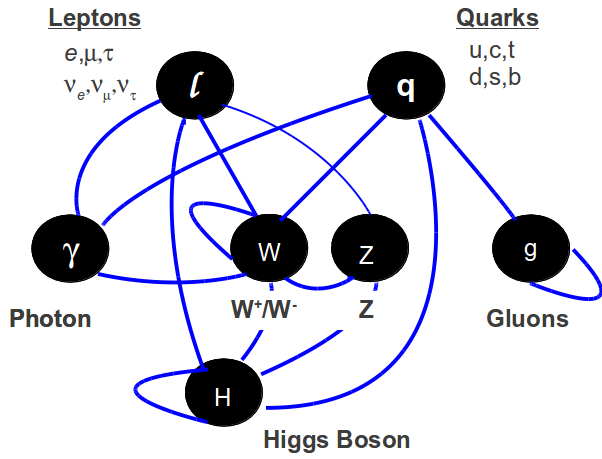
\includegraphics[scale=0.65]{Figures/SM_Interactions.png} 
       \caption[The particles of the Standard Model and their permitted interactions]{The particles of the SM depicted with all tree level permitted interactions.  The top row contains the fermions, the center row contains the force mediating bosons, and the bottom row contains the Higgs boson.}
\label{figapp:SMInteractions}
\end{figure}


\subsection{Beyond the Standard Model}

While the Standard Model has been heavily probed by experiments and proves to be a very powerful predictive tool, it does have numerous limitations.  It possesses no description of the force of gravity whatsoever, despite its considerations of every other known fundamental force.  Explanations have been attempted to account for this via the combination of principles of supersymmetry and gravity known as ``supergravity'' theories, or SUGRA.  Of those fundamental forces, the Standard Model accounts for the relative strengths of the electromagnetic, weak, and strong forces but cannot do so for the difference between the electroweak force strength and the gravitational.  This difference is known as the ``hierarchy problem'' and is also closely tied to the problem of large radiative corrections to the Higgs mass (a ``fine-tuning'' problem).  Additionally, the SM and the Higgs mechanism specifically predict massive leptons with massless neutrinos, which conflicts with the experimentally confirmed model of neutrino oscillation.  

In addition to these problems, the SM leaves open a few compelling questions.  One question, first revealed by the field of astrophysics, is that of dark matter.  Observations of rotation curves of galaxies indicated that nonluminal mass must be present.  An alternative theory of modified Newtonian dynamics was proposed, but then disproven initially by observations of the Bullet cluster and later by other similar phenomena.  The Bullet cluster data showed gravitational lensing occurring in nonluminous regions of two colliding galaxies, which made the issue of actual nonluminal matter concrete.  Measurements of the quantity of our universe that is made of dark matter indicate that it is actually the majority of all matter in our universe, and there is no mechanism in the SM that could explain that fact.  While neutrinos qualify for the qualitative properties of dark matter they cannot explain the quantity of mass that must be nonluminal, and thus there is no dark matter ``candidate'' particle present in the SM.  Numerous models beyond the SM (BSM) contain such candidates, such as supersymmetry and string theory.  Additional questions raised in astrophysics that the SM cannot explain are the observed rate of expansion and the necessary abundance of ``dark energy'' that contributes to this expansion.

Outside of the field of astrophysics the SM offers an additional question: it lacks any explanation for the symmetry between the three generations of quark pairs and the three generations of lepton pairs.  The existence of this symmetry implies a presence of a mechanism to account for it.  Numerous extensions to the SM contain such a mechanism: a hypothetical new particle that possesses both lepton and quark number.  This particle is called a leptoquark and a search for its decay signatures at the LHC is the main subject of this thesis.


\section{Leptoquarks}

\subsection{Theoretical considerations}
\label{theoreticalconsiderations}

Various extensions to the SM include predictions of new bosons that carry both lepton and baryon number, motivated by the essential symmetry of leptons and quarks in it.  Triangle anomalies that otherwise threaten the renormalizability of the SM are canceled by the requirement

\begin{equation}
\sum_{n} Q^{2}_{en} (Q_{L}-Q_{R})_{n} = 0
\label{eq:TriangleCancellation}
\end{equation}

for each of the three fermionic families, where $Q_{en}$, $Q_{Ln}$, and $Q_{Rn}$ denote the elecromagnetic, left-, and right-handed neutral current charges~\cite{Blumlein:1996qp}.  


These new bosons, called leptoquarks (LQ) are hypothetical color-triplet bosons with spin 0 (scalar LQ) or 1 (vector LQ) that are predicted by many extensions of the
standard model (SM) of particle physics, such as Grand Unified Theories~\cite{PhysRevLett.32.438,Pati:1973uk,Pati:1974yy,Murayama:1991ah,Fritzsch:1974nn,Senjanovic:1982ex,PhysRevLett.65.2209,Frampton:1990hz}, technicolor schemes~\cite{Dimopoulos:1979es,Dimopoulos:1979sp,Farhi:1980xs}, and composite models~\cite{Schrempp:1984nj}. They carry fractional electric charge ($\pm \frac{1}{3}$ for LQs considered in this paper) and both baryon and lepton numbers and thus couple to a lepton
and a quark.  Existing experimental
limits on flavor changing neutral currents and other
rare processes disfavor leptoquarks that couple to a quark and lepton of a different SM generation or of more than one SM generation~\cite{Buchmuller:1986iq,FCNC}.  

The description of the LQ phenomenology considered in this thesis begins with an effective lagrangian put forth by W. Buchmuller, R. Ruckl, and D. Wyler in 1986 in the lead up to the turning on of the HERA collider.  ~\cite{Belyaev:2005ew,Buchmuller:1986zs} with the general dimensionless SU(3) $\times$ SU(2) $\times$ U(1) invariant couplings of scalar and vector leptoquarks to leptons and quarks, satisfying baryon and lepton number conservation:


\begin{equation}
\mathcal{L} = \mathcal{L}^{f}_{|\text{F}|=0} + \mathcal{L}^{f}_{|\text{F}|=2}
\label{eq:LQsmalllagrangian}
\end{equation}

The $\mathcal{L}^{f}_{|\text{F}|=0,2}$ Lagrangians describe the Yukawa interactions of LQs with leptons and quarks, changing the fermion number $F$ by 0 or 2, where $F=3B+L$, $B$ is the baryon number and $L$ is the leptons number.  $\mathcal{L}^{f}_{|\text{F}|=0,2}$ are diagonal in flavor:


%%Note: In the paper by S. Belyaev, S and R are both scalar and V and U are both vector
%Also, rather than subscripts denoting the weak isospin, subscripts denote the *dimension* of the weak isospin represatation, thus, following:
% N= 2*I+1
% We have 0->1, 1/2->1, 1->3 to convert from this subscript to S. Belyaev's

\begin{eqnarray}
\mathcal{L}^{f}_{|\text{F}|=0} &=& (h_{2L}\bar{u}_{R}\ell_{L}+h_{2R}\bar{q}_{L}i\sigma_{2}e_{R})S_{\frac{1}{2}} +\tilde{h}_{2L}\bar{d}_{R}\ell_{L}\tilde{S_{\frac{1}{2}}} \nonumber\\
&& +(h_{1L}\bar{q}_{L}\ell_{L}+h_{1R}\bar{d}_{R}\gamma^{\mu}e_{R})V_{0\mu} +\tilde{h}_{1R}\bar{u}_{R}\gamma^{\mu}e_{R}\tilde{V}_{0\mu} \nonumber\\
&&+h_{3L}\bar{q}_{L}\vec{\sigma}\gamma^{\mu}\ell_{L}\vec{V}_{1\mu} +h.c.
\label{eq:LQlagrangianF0},
\end{eqnarray}


\begin{eqnarray}
\mathcal{L}^{f}_{|\text{F}|=2} &=& (g_{2L}\bar{d}^{c}_{R}\gamma^{\mu}\ell_{L}+g_{2R}\bar{q}^{c}_{L}\gamma^{\mu}e_{R})V_{\frac{1}{2}\mu} + \tilde{g}_{2L}\bar{u}^{c}_{R}\gamma^{\mu}\ell_{L}\tilde{V}_{\frac{1}{2}\mu} \nonumber \\
&& +(g_{1L}\bar{q}^{c}_{L}i\sigma_{2}\ell_{L}+g_{1R}\bar{u}^c_{R}e_{R})S_{0}+\tilde{g}_{1R}\bar{d}^c_{R}e_{R}\tilde{S}_{0}  \nonumber \\
&& +g_{3L}\bar{q}^{c}_{L}i\sigma_{2}\vec{\sigma}\ell_{L}\vec{S}_{1} +h.c.
\label{eq:LQlagrangianF2},
\end{eqnarray}

where $q_L$ and $\ell_L$ are the left handed quark and lepton SU(2) doublets, and $e_R$, $d_R$, $u_R$ are the right handed charged leptons, down-, and up-quarks, respectively.  Charge conjugated fields are denoted by $\psi_c=\bar{\psi}^T$, $\sigma_i$ are the Pauli spin matrices.  The subscripts L, R, of the coupling constants $g_{i}$ and $h_{i}$ denote the lepton chirality.  The LQ indices give the weak isospin.  



\begin{table}[!Hhtbp]
\begin{tabular}{|c|ccccc|ccc|c|}
\hline
{LQ type}  & {$Q_{em}$}& {$T_{3}$}& {$T$} &{$Y$}& {F=3B+L}& {$\lambda_{L}(\ell q)$}& {$\lambda_{L}(\nu q)$}& {$\lambda_{R}(\ell q)$}&{Final States}\\
\hline
\hline
{$S_{0,L}$}  & {$1/3$}& {$0$}& {$0$} &{$2/3$}& {$-2$}& {$g_{1L}$}& {$-g_{1L}$}& {$0$}&{$\ell^{+}_{L}\bar{u}_{L},\bar{\nu}_{L}\bar{d}_{L}$}\\
\hline
{$S_{0,R}$}  & {$1/3$}& {$0$}& {$0$} &{$2/3$}& {$-2$}& {$0$}& {$0$}& {$g_{1R}$}&{$\ell^{+}_{R}\bar{u}_{R}$}\\
\hline
{$\tilde{S}_{0,R}$}  & {$4/3$}& {$0$}& {$0$} &{$8/3$}& {$-2$}& {$0$}& {$0$}& {$\tilde{g}_{1R}$}&{$\ell^{+}_{R}\bar{d}_{R}$}\\
\hline
{$S_{\frac{1}{2},L}$}  & {$5/3$}& {$1/2$} & \multirow{2}{*}{$1/2$}&\multirow{2}{*}{$7/3$}& \multirow{2}{*}{$-2$}& {$h_{2L}$}& {$0$}& {$0$}&{$\ell^{+}_{L}u_{L}$}\\
{$S_{\frac{1}{2},L}$}  & {$2/3$}& {$-1/2$} & {}&{}& {}& {$0$}& {$h_{2L}$}& {$0$}&{$\bar{\nu}_{L}u_{L}$}\\
\hline
{$S_{\frac{1}{2},R}$}  & {$5/3$}& {$1/2$} & \multirow{2}{*}{$1/2$}&\multirow{2}{*}{$7/3$}& \multirow{2}{*}{$-2$}& {$0$}& {$0$}& {$h_{2R}$}&{$\ell^{+}_{R}u_{R}$}\\
{$S_{\frac{1}{2},R}$}  & {$2/3$}& {$-1/2$} & {}&{}& {}& {$0$}& {$0$}& {$-h_{2R}$}&{$\ell^{+}_{R}d_{R}$}\\
\hline
{$\tilde{S}_{\frac{1}{2},L}$}  & {$2/3$}& {$1/2$} & \multirow{2}{*}{$1/2$}&\multirow{2}{*}{$1/3$}& \multirow{2}{*}{$-2$}& {$\tilde{h}_{2L}$}& {$0$}& {$0$}&{$\ell^{+}_{L}d_{L}$}\\
{$\tilde{S}_{\frac{1}{2},L}$}  & {$-1/3$}& {$-1/2$} & {}&{}& {}& {$0$}& {$\tilde{h}_{2L}$}& {$0$}&{$\bar{\nu}_{L}d_{L}$}\\
\hline
{$S_{1,L}$}  &{$4/3$}& {$1$} & \multirow{3}{*}{$1$}&\multirow{3}{*}{$2/3$}& \multirow{3}{*}{$-2$}& {$-\sqrt{2}g_{3L}$}& {$0$}& {$0$}&{$\ell^{+}_{L}\bar{d}_{L}$}\\
{$S_{1,L}$}  &{$1/3$}& {$0$} &&&& {$-g_{3L}$}& {$0$}& {$-g_{3L}$}&{$\ell^{+}_{L}\bar{u}_{L},\bar{\nu}_{L}\bar{d}_{L}$}\\
{$S_{1,L}$}  &{$-2/3$}& {$-1$} &&&& {$$}& {$0$}& {$\sqrt{2}g_{3L}$}&{$\bar{\nu}_{L}\bar{u}_{L}$}\\

\hline
\hline
{$V_{0,L}$}  & {$2/3$}& {$0$}& {$0$} &{$4/3$}& {$-2$}& {$h_{1L}$}& {$h_{1L}$}& {$0$}&{$\ell^{+}_{L}d_{R},\bar{\nu}_{L}u_{R}$}\\
\hline
{$V_{0,R}$}  & {$2/3$}& {$0$}& {$0$} &{$4/3$}& {$-2$}& {$0$}& {$0$}& {$h_{1R}$}&{$\ell^{+}_{R}d_{L}$}\\
\hline
{$\tilde{V}_{0,R}$}  & {$5/3$}& {$0$}& {$0$} &{$10/3$}& {$-2$}& {$0$}& {$0$}& {$\tilde{h}_{1R}$}&{$\ell^{+}_{R}u_{L}$} \\
\hline
{$V_{\frac{1}{2},L}$}  & {$4/3$}& {$1/2$} & \multirow{2}{*}{$1/2$}&\multirow{2}{*}{$5/3$}& \multirow{2}{*}{$-2$}& {$g_{2L}$}& {$0$}& {$0$}&{$\ell^{+}_{L}\bar{d}_{R}$}\\
{$V_{\frac{1}{2},L}$}  & {$1/3$}& {$-1/2$} & {}&{}& {}& {$0$}& {$g_{2L}$}& {$0$}&{$\bar{\nu}_{L}\bar{d}_{R}$}\\
\hline
{$V_{\frac{1}{2},R}$}  & {$4/3$}& {$1/2$} & \multirow{2}{*}{$1/2$}&\multirow{2}{*}{$5/3$}& \multirow{2}{*}{$-2$}& {$0$}& {$0$}& {$g_{2R}$}&{$\ell^{+}_{R}\bar{d}_{L}$}\\
{$V_{\frac{1}{2},R}$}  & {$1/3$}& {$-1/2$} & {}&{}& {}& {$0$}& {$0$}& {$g_{2R}$}&{$\ell^{+}_{R}\bar{u}_{L}$}\\
\hline
{$\tilde{V}_{\frac{1}{2},L}$}  & {$1/3$}& {$1/2$} & \multirow{2}{*}{$1/2$}&\multirow{2}{*}{$-1/3$}& \multirow{2}{*}{$-2$}& {$\tilde{g}_{2L}$}& {$0$}& {$0$}&{$\ell^{+}_{L}\bar{u}_{R}$}\\
{$\tilde{V}_{\frac{1}{2},L}$}  & {$-2/3$}& {$-1/2$} & {}&{}& {}& {$0$}& {$\tilde{g}_{2L}$}& {$0$}&{$\bar{\nu_{L}}\bar{u}_{R}$}\\
\hline
{$V_{1,L}$}  &{$5/3$}& {$1$} & \multirow{3}{*}{$1$}&\multirow{3}{*}{$4/3$}& \multirow{3}{*}{$-2$}& {$\sqrt{2}h_{3L}$}& {$0$}& {$0$}&{$\ell^{+}_{L}u_{R}$}\\
{$V_{1,L}$}  &{$2/3$}& {$0$} &&&& {$-h_{3L}$}& {$0$}& {$h_{3L}$}&{$\ell^{+}_{L}\bar{d}_{R},\bar{\nu}_{L}u_{R}$}\\
{$V_{1,L}$}  &{$-1/3$}& {$-1$} &&&& {$$}& {$0$}& {$\sqrt{2}h_{3L}$}&{$\bar{\nu}_{L}d_{R}$}\\

\hline


\end{tabular}
\\
\caption[The types of scalar and vector LQs with their quantum numbers, coupling strenths, and final state decay modes]{Scalar (S) and vector (V) type LQs, with their quantum numbers, coupling strengths, and final state decay modes.  Quantum numbers given are fermion number (F), hypercharge (Y), weak isospin ($T$), the third component of weak isospin ($T_{3}$), and electric charge ($Q_{em}$).}
\label{tab:LQTable}
\end{table}


\subsection{Signatures at the LHC}
In pp collisions LQs can be produced either singly or in pairs, with very similar final state decay products.  In pair production, LQs are produced predominantly via gluon-gluon fusion with additional contributions from quark-quark annihilation, as indicated in Eq.~\ref{eq:PairLQ1} and Eq.~\ref{eq:PairLQ2}


\begin{equation}
g+g\rightarrow \text{LQ}+\overline{\text{LQ}}
\label{eq:PairLQ1}
\end{equation}



\begin{equation}
q+\overline{q}\rightarrow \text{LQ}+\overline{\text{LQ}}
\label{eq:PairLQ2}
\end{equation}

These decay modes result in a final state of two leptons and two jets.  Single production of LQs occurs in association with a lepton via quark-gluon fusion, as indicated in Eq.~\ref{eq:SingleLQ1}, and thus results in a final state of two leptons and one jet.



\begin{equation}
q+g\rightarrow \text{LQ}+\ell
\label{eq:SingleLQ1}
\end{equation}

Of all the diagrams contributing to pair production, only one posseses any $\lambda$-dependance at all and the overall dependence on $\lambda$ in pair production is negligible~\cite{Hewett:1997ce}.  In contrast to this single production diagrams, depicted in Figures~\ref{figapp:schanneldiag} through~\ref{figapp:tchannel2diag}, do scale with the coupling.  Single production cross sections decrease more slowly with the coupling, exceeding pair production at an order of 1 TeV for $\lambda = 0.6$.  


\begin{figure}[!Hh]
       \centering
       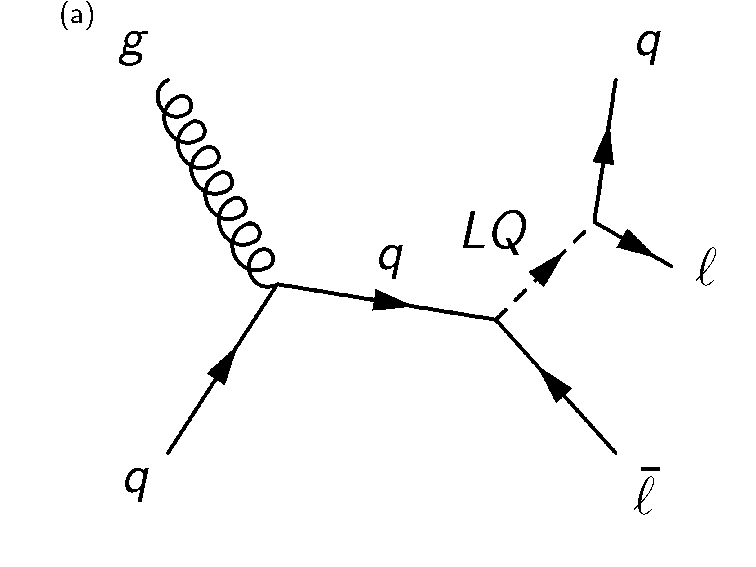
\includegraphics[scale=0.65]{Figures/schannel.pdf} 
       \caption[The $s$-channel resonant LQ production diagram.]{The $s$-channel resonant LQ production diagram.}
\label{figapp:schanneldiag}
\end{figure}


\begin{figure}[!Hh]
       \centering
       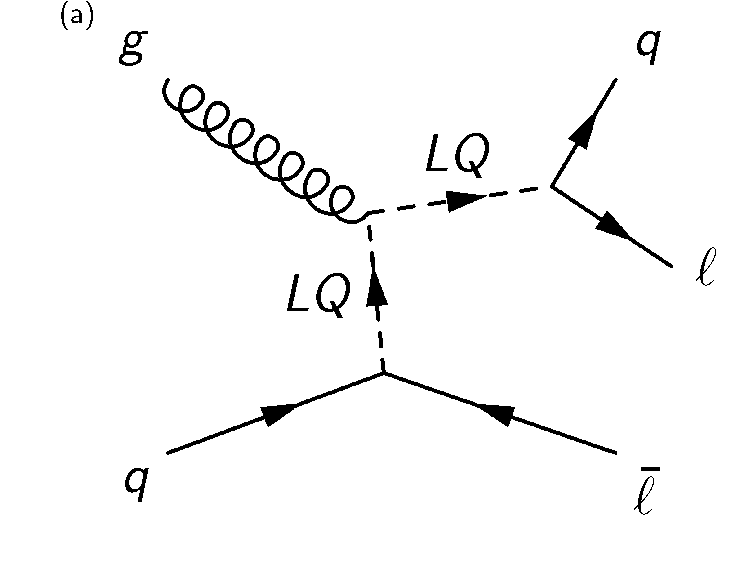
\includegraphics[scale=0.65]{Figures/tchannel1.pdf} 
       \caption[The $t$-channel LQ production diagram with a resonant production component.]{The $t$-channel LQ production diagram with a resonant production component.}
\label{figapp:tchannel1diag}
\end{figure}


\begin{figure}[!Hh]
       \centering
       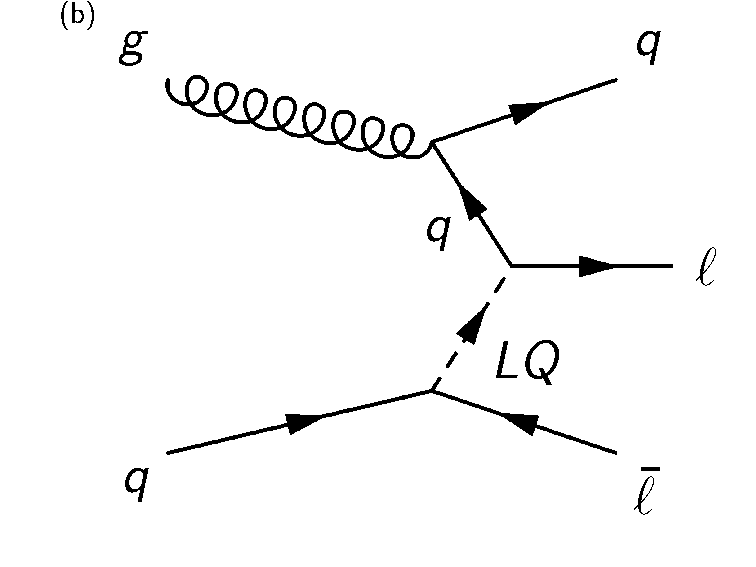
\includegraphics[scale=0.65]{Figures/tchannel2.pdf} 
       \caption[The $t$-channel nonresonant LQ production diagram.]{The $t$-channel nonresonant LQ production diagram.}
\label{figapp:tchannel2diag}
\end{figure}

The main single leptoquark production mode at the LHC is the resonant diagram shown in
Figure~\ref{figapp:schanneldiag}. However, significant contributions are made by the diagrams with non-resonant com-
ponents shown in Figures~\ref{figapp:tchannel1diag} and~\ref{figapp:tchannel2diag}. These contributions increase with both the LQ mass and coupling;
the invariant mass distribution of a first generation LQ, of LQ mass $M_{\text{LQ}}$ = 1 TeV and coupling
$\lambda$ = 1.0, possesses a tail that extends to very low masses that is comparable to the peak in
magnitude.  

Due to the parton distribution function dependence of single LQ production, the cross sections for second generation LQs is significantly suppressed with respect to first generation LQs.  

The signatures for LQ single production include three-object final states with leptons ($\ell$), neutrinos ($\nu$), and a single jet ($j$).  There are two distinct final state signatures, $\ell^{+} \ell^{-} j$ and $\nu \nu j$.  This thesis considers single LQ production with $\beta=1.0$, thus only final state signatures with two leptons and a jet.  The major SM backgrounds that can mimic this signature are Z boson production in association with one or more jets and $t\bar{t}$ production.  In the case of Z boson production, the Z decays to two leptons yielding the same final state particles as single LQ production.  There are three possible decay modes for $t\bar{t}$ production: fully leptonic, partially leptonic, and hadronic.  It is the fully leptonic mode, $t\bar{t} \rightarrow bW(\rightarrow\ell\nu)bW(\rightarrow\ell\nu)$ that can mimic single LQ production with two charged leptons, although it does also possess additional missing transverse energy from the neutrinos.  Other SM processes that are additional small contributions to the total background that of events with two charged leptons and at least one jet are diboson (WW, WZ,ZZ) production, single t-quark production, and QCD multijet production in which two jets are misidentified as leptons.  



\subsection{Previous searches}

In addition to the indirect limits that restrict LQs to coupling to same-generation leptons discussed in Section~\ref{theoreticalconsiderations}, various collaborations have performed direct searches for LQs.  

Early searches for scalar leptoquarks were conducted at the HERA $ep$ collider by the H1~\cite{Aid:1995wd,Abt:1993nr,Collaboration:2011qaa} and ZEUS~\cite{Derrick:1993by} collaborations and found no evidence for leptoquarks.  Limits were set at 95\% confidence level of $M_{\text{LQ}}(\text{1st gen.}) < 250$ GeV for $|F|=0$ with the assumption that $\lambda > \lambda_{em}$.  Later results in 1997 from the HERA collider had intriguing implications for leptoquarks and increased interest in searches for them.  Both the H1 and ZEUS collaborations reported excesses in neutral current deep inelastic scattering events ($e^+ p \rightarrow e^+ X$) at high values of $Q^2$, where $Q^2$ is the four-momentum transfer~\cite{H1excess,ZEUSexcess}.  Figure~\ref{figapp:Q2excess} depicts the excess measured by the H1 collaboration, showing both the total number of events measured and the ratio to the SM expectation versus $Q^2$.  The reconstructed invariant mass of the final state electron and jet is compared to the SM expectation in Figure~\ref{figapp:Q2excess} with an excess visible at high values of $Q^2$, concentrated near values of $M_{e^+ j}$ of 200 GeV.  

Searches for LQs following the observation of this excess have ruled out LQs at various detectors.  The D$0$ collaboration produced limits on singly first generation LQs of $M_{\text{LQ}} > 274$ GeV ($\lambda=1.0$ and $\beta=1.0$) ~\cite{Abazov:2006ej}.  In 2011, the H1 collaboration published comprehensive limits on singly produced LQs of various types as a function of $\lambda$~\cite{Collaboration:2011qaa}, placing a limit on the $S^{R}_{0}$ type LQ that this thesis primarily considers of  $M_{\text{LQ}} > 500$ GeV ($\lambda=1.0$ and $\beta=1.0$).  These limits are shown in Figure~\ref{figapp:H1limits}.  


\textcolor{red}{FIXME: 2012 CMS results.}  %Data being collected at this very moment at a center of mass energy of 13 TeV comprise data collected on collisions at the highest energies performed to this date.  This increase in energy roughly doubles the single LQ production cross sections at the LHC, allowing for greater reach for this statistically limited search.

The 20 $fb^{-1}$ of data collected by CMS with a center-of-mass energy of $\sqrt{s}=8$\TeV is unprecedented for hadron colliders, both with respect to total integrated luminosity and collision energy.  For a statistically limited search such as the search for single LQ production, this provides significantly greater reach than achieved in the past at other colliders.  Additionally, advances in detector technology, described in Chapter 2, and in reconstruction, described in Chaper 3, provide the ability to even more precisely measure particle kinematics.  These techniques along with the increase in integrated luminosity also create a reduction of the systematic uncertainties associated with measurements made with the CMS detector.  

In this thesis, a search for single production of first- and second-generation scalar LQs with the CMS detector is presented, as a function of LQ mass and coupling $\lambda$, using all the 8 TeV collision data collected.  The SM backgrounds are studied in detail, and data-driven methods for estimating the most significant backgroudns are utilized.  


\begin{figure}[!Hh]
       \centering
       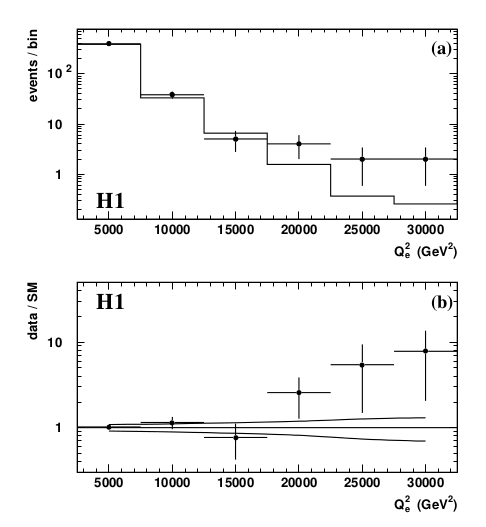
\includegraphics[scale=0.65]{Figures/H1Excess_Q2.png} 
       \caption[Excesses measured by the H1 collaboration in the $Q^2$ distribution of neutral current deep inelastic scattering events]{Observation of an excess of high $Q_e^2$ events measured by the H1 collaboration, where the subscript $e$ represents the ``e-method'' used to compute $Q^2$, using only information from the scattered electron~\cite{H1excess}.  The number of events is shown in (a), with the solid black circles representing data and the solid black line representing the neutral current deep inelastic scattering expectation.  The ratio of data over expectation is shown in (b), with the lines above and below unity representing the $\pm1\sigma$ levels calculated including both statistical and systematic errors of the expected values.}
\label{figapp:Q2excess}
\end{figure}


\begin{figure}[!Hh]
       \centering
       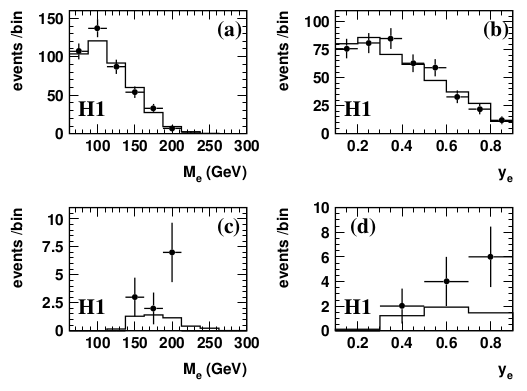
\includegraphics[scale=0.85]{Figures/H1Excess_M.png} 
       \caption[Excesses measured by the H1 collaboration in the mass and $y$ distributions of neutral current deep inelastic scattering events]{Obseravtion of an excess in the $M_e$ distribution at high values of $Q_e^2$.  The subscript $e$ represents the ``e-method'' used to compute $Q^2$, using only information from the scattered electron~\cite{H1excess}.  Distributions of $M_e$ and $y_e$ (where $y_e$ is the the ratio of the electron four momentum over the jet four-momentum) of events with $2500 \text{GeV} < Q_e^2 < 15000 \text{GeV}$ are shown in (a) and (b), respectively.  The same distributions for $Q_e^2 > 15000 \text{GeV}$ are shown in (c) and (d).}
\label{figapp:Q2excess}
\end{figure}




\begin{figure}[!Hh]
       \centering
       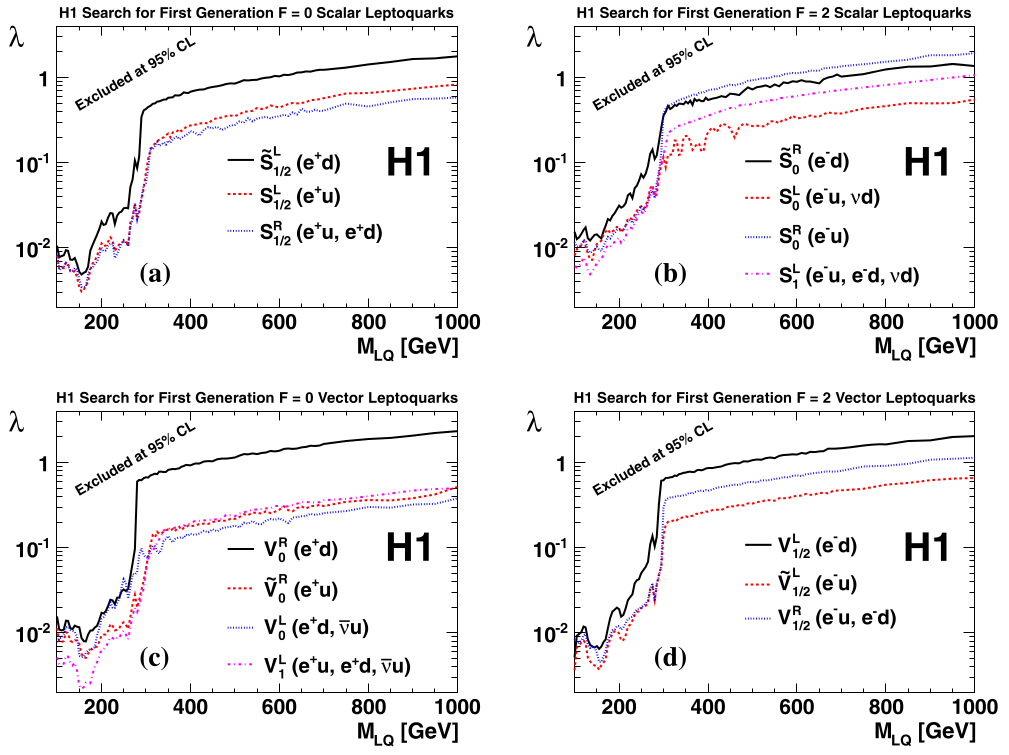
\includegraphics[scale=0.45]{Figures/H1limits.png} 
       \caption[Observed limits on LQs produced by the H1 collaboration]{Exclusion limits produced by the H1 collaboration, for all 14 LQ types as described by the LQ model in Section \label{theoreticalconsiderations}.  The limits are expressed on $\lambda$ as a function of LQ mass, for scalar LQs with F = 0 (a) and F = 2 (b) as well as for vector LQs with F = 0 (c) and F = 2 (d).  The domains above the curves are excluded at 95\% confidence level.}
\label{figapp:H1limits}
\end{figure}

% Chapter 2

\chapter{The Experimental Apparatus} % Main chapter title

\label{apparatus} % For referencing the chapter elsewhere, use \ref{Chapter1} 

\lhead{Chapter 2. \emph{The Experimental Apparatus}} % This is for the header on each page - perhaps a shortened title

%----------------------------------------------------------------------------------------

This chapter describes the Large Hadron Collider (LHC)~\cite{LHCmachine} and the Compact Muon Solenoid (CMS)~\cite{CMSdetector} detector which records data from pp and heavy ion collisions and is located at one of the main interaction points along the LHC.  The CMS detector is a general-purpose detector that recorded data from 2010 to 2012 corresponding to 36 $\text{pb}^{-1}$ and 5 $\text{fb}^{-1}$ at $\sqrt{7}$ TeV and 19.6 $\text{fb}^{-1}$ at $\sqrt{8}$ TeV.  Section~\ref{lhcsection} contains details on the design and specifications of the LHC and section~\ref{cmssection} describes the CMS detector, its sub-systems, and a number of upgrades (both completed and planned) that it has undergone.

\section{The Large Hadron Collider}
\label{lhcsection}

The LHC is a two-ring-superconducting-hadron accelerator and collider that sits in the 26.7 km tunnel that was constructed for and housed the Large Electron Positron collider (LEP).  It is capable of delivering pp, lead-lead, and proton-lead collisions.  This section will focus on pp collisions.

\subsection{Design}

In 1994 the proposal to the CERN council to construct the LHC in the existing LEP tunnel was approved.  With the Superconducting Super Collider (SSC) canceled just the year before due to concerns related to rising costs, the ability to use a preexisting tunnel was a significant motivation for construction of the LHC to be located there.  As a result the layout of the LHC was strongly influenced by geometry of the LEP tunnel.

Before reaching the full collision energies, particles in the LHC must go through a series of accelerators in which they are successively brought to higher and higher energies.  This system, composed of an initial linear accelerator and a number of synchrotrons, is called the injection chain and consists of the following systems:

\begin{itemize}
\item The linear accelerators (LINACs) are the first step in the chain.  The LINAC2 accelerator generates the protons at an energy of 50 MeV for injection in to the smallest synchrotron.
\item The Proton Synchrotron Booster (PSB) prepares the protons for injection in to the next step, the Proton Synchrotron (PS).  In it the protons are accelerated to 1.4 GeV.
\item The PS then raises the proton energy to 26 GeV.
\item The last step before injection in to the LHC itself, the Super Proton Synchrotron (SPS) accelerates the proton beams to 450 GeV.
\item Finally, once in the LHC, the proton beams are accelerated to the energies at which they will collide.  In 2010 and 2011 the operating energy here was 3.5 TeV, in 2012 the energy per beam was increased to 4 TeV.  Currently, in 2015, the proton beams circulating in the LHC each possess an energy of 6.5 TeV.
\end{itemize}

These accelerators are depicted in Figure~\ref{figapp:LHCinjection} with their approximate relative sizes and locations.

\begin{figure}[!Hh]
       \centering
       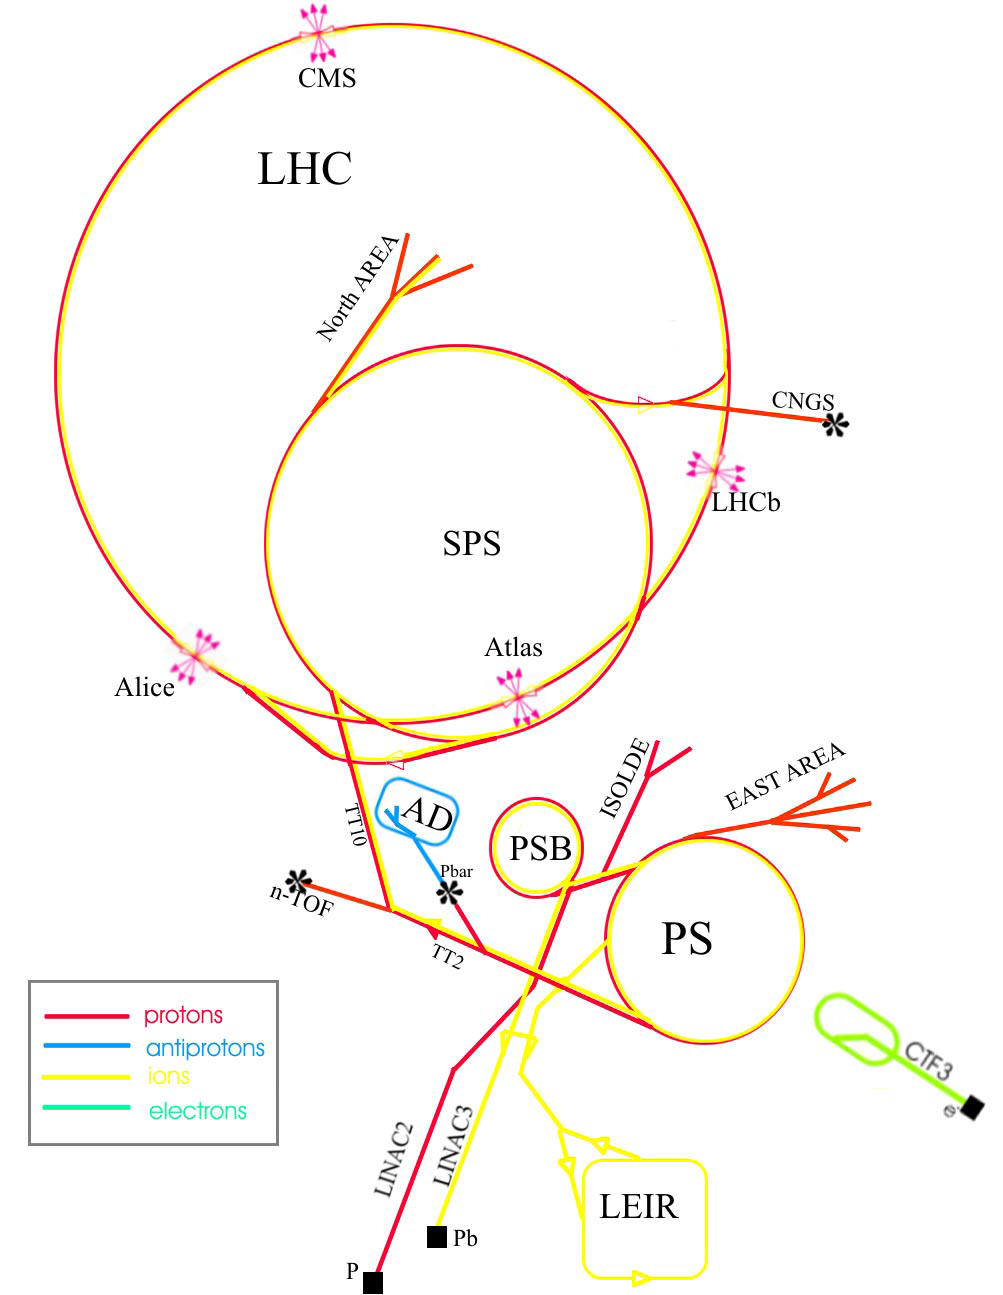
\includegraphics[scale=0.1]{Figures/PSnew.jpg} 
       \caption[Schematic of the LHC injection chain system.]{A schematic of the injection chains of the successive accelerators in to the LHC.  The LINACs at the bottom of the diagram inject the protons or the lead ions which enter the LHC via the PSB, PS, and SPS.  The approximate relative size of each system is shown, as well as relative locations.}
\label{figapp:LHCinjection}
\end{figure}


Once accelerated to these energies the beams are made to collide at four points along the LHC ring.  The LHC has eight arcs and eight straight sections.  Each straight section is 528 m long and can serve as an experimental or insertion point.  Point 1, in the center of the first ``octant'', is the location of the ATLAS (A Toroidal LHC Apparatus) experiment, while CMS is located across the LHC ring at Point 5.  Points 2 and 8 are the locations of the ALICE (A Large Ion Collider Experiment) and LHCb (LHC beauty) experiments, as well as the injection points for Beam 1 and Beam 2 (the main colliding beams used in the LHC).  These 4 points are where the beams cross at interaction points (IPs), where the $\beta$ function is low and the beams are squeezed.  The remaining 4 octants do not contain IPs, rather Points 3 and 7 contain collimations systems, Point 4 contains an RF system, and Point 6 is the location of the beam dump system.  This consists of a combination of horizontally deflecting fast-pulsed magnets and vertically deflecting double steel septum magnets that serve to vertically extract both beams~\cite{LHCmachine}.  This layout is depicted in Figure~\ref{figapp:LHClayout}.



\begin{figure}[!Hh]
       \centering
       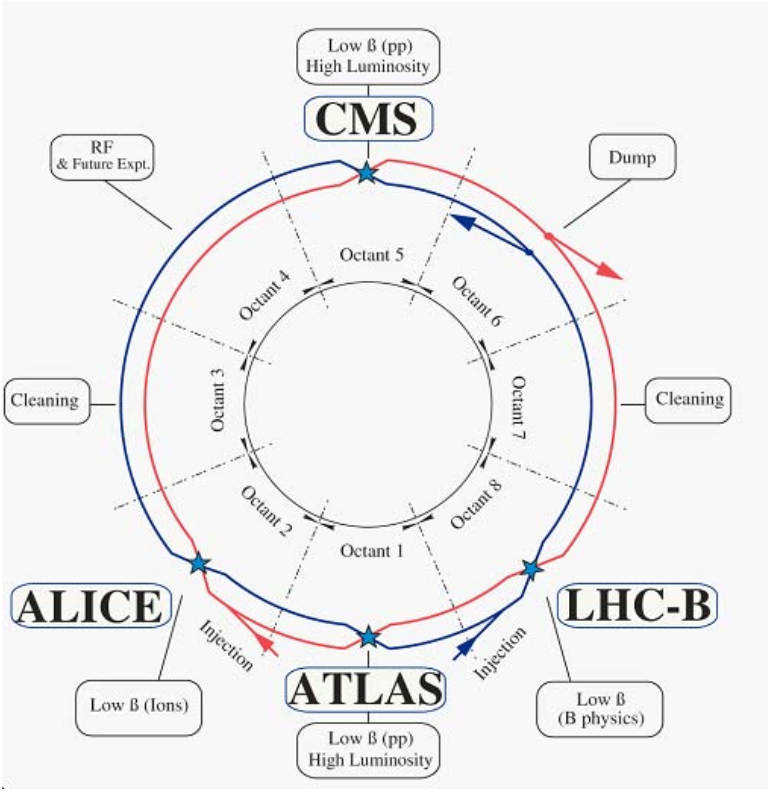
\includegraphics[scale=0.5]{Figures/LHClayout.png} 
       \caption[Schematic of the LHC layout.]{A schematic of the layout of the LHC.  Points 1, 2, 5, and 8 are the locations of the 4 experiments conducted at the LHC~\cite{LHCmachine}.}
\label{figapp:LHClayout}
\end{figure}

Each of the eight arcs that compose the majority of the LHC's 26.7 km is composed of 23 cells, each 106.9 m long, making each arc approximately 2.5 km in length.  Each arc cell itself is composed of two half cells each containing a cold mass (6.63 m long cryostat), a short straight section (SSS), and three dipole magnets 14.3 m in length.  This comes to a total of 1104 main dipoles in use in the LHC ring straight sections and with 128 more in use in the straight regions the LHC contains 1232 dipole magnets in total.  Each dipole is held to a temperature of 1.9 K in operation and provides a magnetic field (at the 7 TeV beam energy) of 8.33 T.  At this operating level the current through the dipole magnets is 11.85 kA.  The layout of the dipole magnets is given in Figure~\ref{figapp:LHCdipole}.  The SSSs contain the main quadrupole magnets and a variety of magnets such as skew quadrupole correctors, sextupole-dipole correctors, tuning quadrupoles, and octupoles.  


\begin{figure}[!Hh]
       \centering
       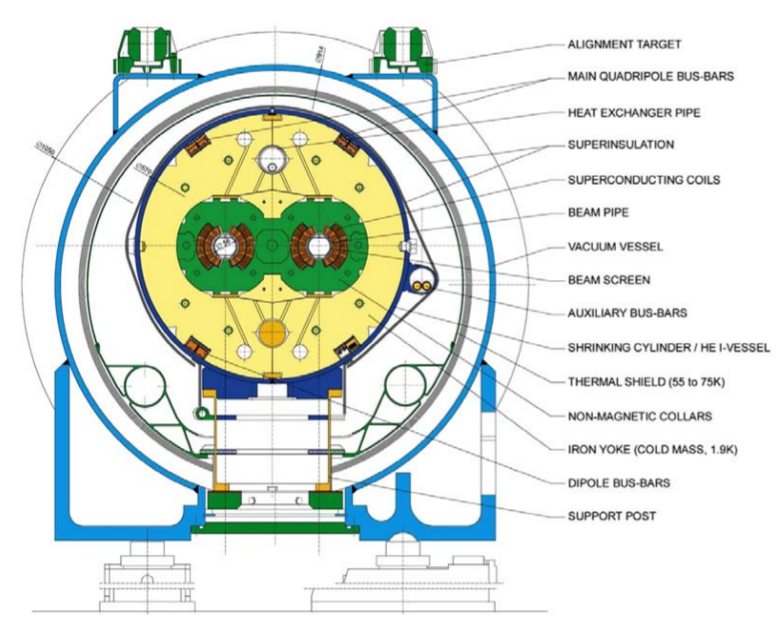
\includegraphics[scale=0.5]{Figures/LHCdipole.png} 
       \caption[Diagram of an LHC cryodipole.]{Diagram of a cross section of an LHC ``cryodipole'': the combined assembly housing the superconducting dipole magnets and the cold mass~\cite{LHCmachine}.}
\label{figapp:LHCdipole}
\end{figure}


\subsection{Specifications and parameters}

The aim of the LHC being to reveal physics beyond the standard model, not only must the beam energy be high to reveal processes suppressed in nature due to kinematics, but also integrated luminosity is a limiting variable for statistically limited searches.  The integrated luminosity over a period of time, $T$, is given by:

\begin{equation}
\mathcal{L} = \int_{T}{\text{L} dt}
\label{eq:IntLuminosity}
\end{equation}

where L is the luminosity and is measured in number of collisions the LHC can produce per unit area per unit time (machine luminosity).  Given a particular physics process of interest, $P$, the number of expected events for such a process over a period of time $T$ is:

\begin{equation}
N_{event}(P) = \int_{T}{\text{L} \sigma_{event}(P) dt}
\label{eq:NumEvents}
\end{equation}

where $\sigma_{event}(P)$ is the cross section for the event of the process in question and depends on the the energy in the event and the model in question.  The instantaneous luminosity, $L$, depends only on the beam parameters and is given by the expression:


\begin{equation}
L = \frac{N^2_b n_b f_{rev} \gamma_r}{4 \pi \epsilon_n \beta^*} F
\label{eq:InstLuminosity}
\end{equation}

where $N_b$ is the number of particles per bunch, $n_b$ is the number of bunches per beam, $f_{rev}$ is the revolution frequency, $\gamma_r$ is the relativistic gamma factor, $\epsilon_n$ is the normalized transverse beam emittance, $\beta^*$ is the beam beta function at the collision point, and F is the geometric luminosity reduction factor due to the crossing angle at the IP.  The value for F is given by the following expression:


\begin{equation}
F = \left(1+\left(\frac{\theta_c \sigma_z}{2 \sigma^*}\right)^2\right)^{-1/2}
\label{eq:BeamF}
\end{equation}

where $\theta_c$ is the full crossing angle at the IP, $\sigma_z$ is the RMS bunch length, and $\sigma^*$ is the transverse RMS beam size at the IP.  This assumes round beams, with $\sigma_z \ll \beta$, as well as assuming equal beam parameters for both beams.  

The discovery of rare processes at the LHC relies upon high energies, high instantaneous luminosities, and significant run times.  The maximum particle density per bunch is limited by nonlinear beam-beam interactions that occur when bunches from the two beams collide with each other.  This beam-beam interaction is measured by the linear tune shift which is given by:



\begin{equation}
\xi = \frac{N_b r_p}{4 \pi \epsilon_n}
\label{eq:LinearTuneShift}
\end{equation}

where $r_p$ is the classical proton radius, $r_p = e^2 / (4 \pi \epsilon_0 m_p c^2)$.  Previous experience with hadron colliders has indicated that the total linear tune shift including all IPs should not exceed 0.015~\cite{LHCmachine}.  The LHC runs pp collisions in 3 experiments simultaneously, so parameters at the LHC must satisfy $\xi < 0.005$.


The LHC beam energy was 3.5 TeV per beam in 2010 and 2011, increasing to 4 TeV in 2012.  The peak instantaneous luminosity during these run periods was a fraction of the nominal value, starting at 2\% in 2010 and increasing to 35\% in 2011 and 77\% in 2012.  The running parameters for 2012 and nominal design conditions are given in Table~\ref{tab:LHCparams}.  Achieving 77\% of nominal with half the nominal number of bunch was achieved partially due to the excellent beam quality delivered by the injectors, yielding an above-nominal number of protons per bunch.  Challenges have arisen, unique to operating complex systems and electronics in the LHC environment.  Occasional beam dumps can be caused by Unidentified Falling Objects (UFOs), and Single Event Effects (SEEs) caused by beam induced radiation to tunnel electronics was a significant source of inefficiency at the onset of the 2011 run~\cite{LHCstatus}.  As the 2015 run is ongoing, with the higher beam energy of 6.5 TeV, UFOs pose an increased challenge to LHC operation.  Looking forward, a series of long shutdowns will prepare the LHC for the High Luminosity LHC program, for which CMS is preparing upgrades to handle and take advantage of the increased rate.  


\begin{table}[!Hhtbp]
\centering
\begin{tabular}{llcc}
\hline
{} & {Parameter}  & {LHC Design Value} &{Achieved in 2012 run}\\
\hline
\hline
{$N_b$} & {Number of particles per bunch} & {$1.15 \times 10^{11}$} &{$1.6-.17 \times 10^{11}$}\\
{$n_b$} & {Number of bunches per beam} & {2808} &{1374}\\
{$f_{rev}$} & {Revolution frequency} & {11.25 kHz} & {11.25 kHz}\\
{$\gamma_r$} & {Relativistic gamma factor} & {7461} &{4263}\\
{$\epsilon_n$} & {Transverse beam emittance} & {$3.75 \mu \text{m}$} &{$2.5 \mu \text{m}$}\\
{$\beta^*$} & {Beta function at IP} & {0.55} &{0.6}\\
{$\theta_c$} & {Crossing angle at IP} & {$285 \mu \text{rad}$} &{$290 \mu \text{rad}$}\\
{$\sigma_z$} & {RMS bunch length} & {7.55 cm} &{9 cm}\\
{$\sigma^*$} & {Transverse RMS beam size at IP} & {$16.6 \mu \text{m}$} &{$19 \mu \text{m}$}\\
{$L$} & {Peak instantaneous luminosity} & {$1 \times 10^{34}$} &{$7.7 \times 10^{33}$}\\
{} & {Bunch spacing} & {25 ns} &{50 ns}\\
{} & {Stored beam energy} & {362 MJ} &{~140 MJ}\\
{} & {Beam energy} & {7 TeV} &{4 TeV}\\
\hline
\end{tabular}
\\
\caption[LHC running parameters, designed and achieved in 2012.]{The targeted design values for the running parameters of the LHC and the values achieved in the 2012 run~\cite{LHCstatus}.}
\label{tab:LHCparams}
\end{table}


\section{The Compact Muon Solenoid}
\label{cmssection}

The IP at Point 5 is the location of the Compact Muon Solenoid (CMS), a general purpose detector used for a variety of higgs and exotic searches and SM measurements.  In 2012, an integrated luminosity of 21.79 $\text{fb}^{-1}$ was recorded by the CMS detector, the integrated luminosity and peak daily luminosities and shown in Figure~\ref{figapp:CMSLumi2012}.  On ~\textcolor{red}{FIXME: Insert date and lumi plots here for 2015 progress} it has recorded a luminosity of ~\textcolor{red}{X} $\text{fb}^{-1}$, shown in Figure~\ref{figapp:CMSLumi2015}.This section describes the CMS detector and its subsystems.  Section\label{cscelectronics} goes in to greater detail regarding the electronics used in the endcap muon subsystem as the author of this thesis was responsible for work on upgrading a component of those systems.  



\begin{figure}[!Hh]
       \centering
       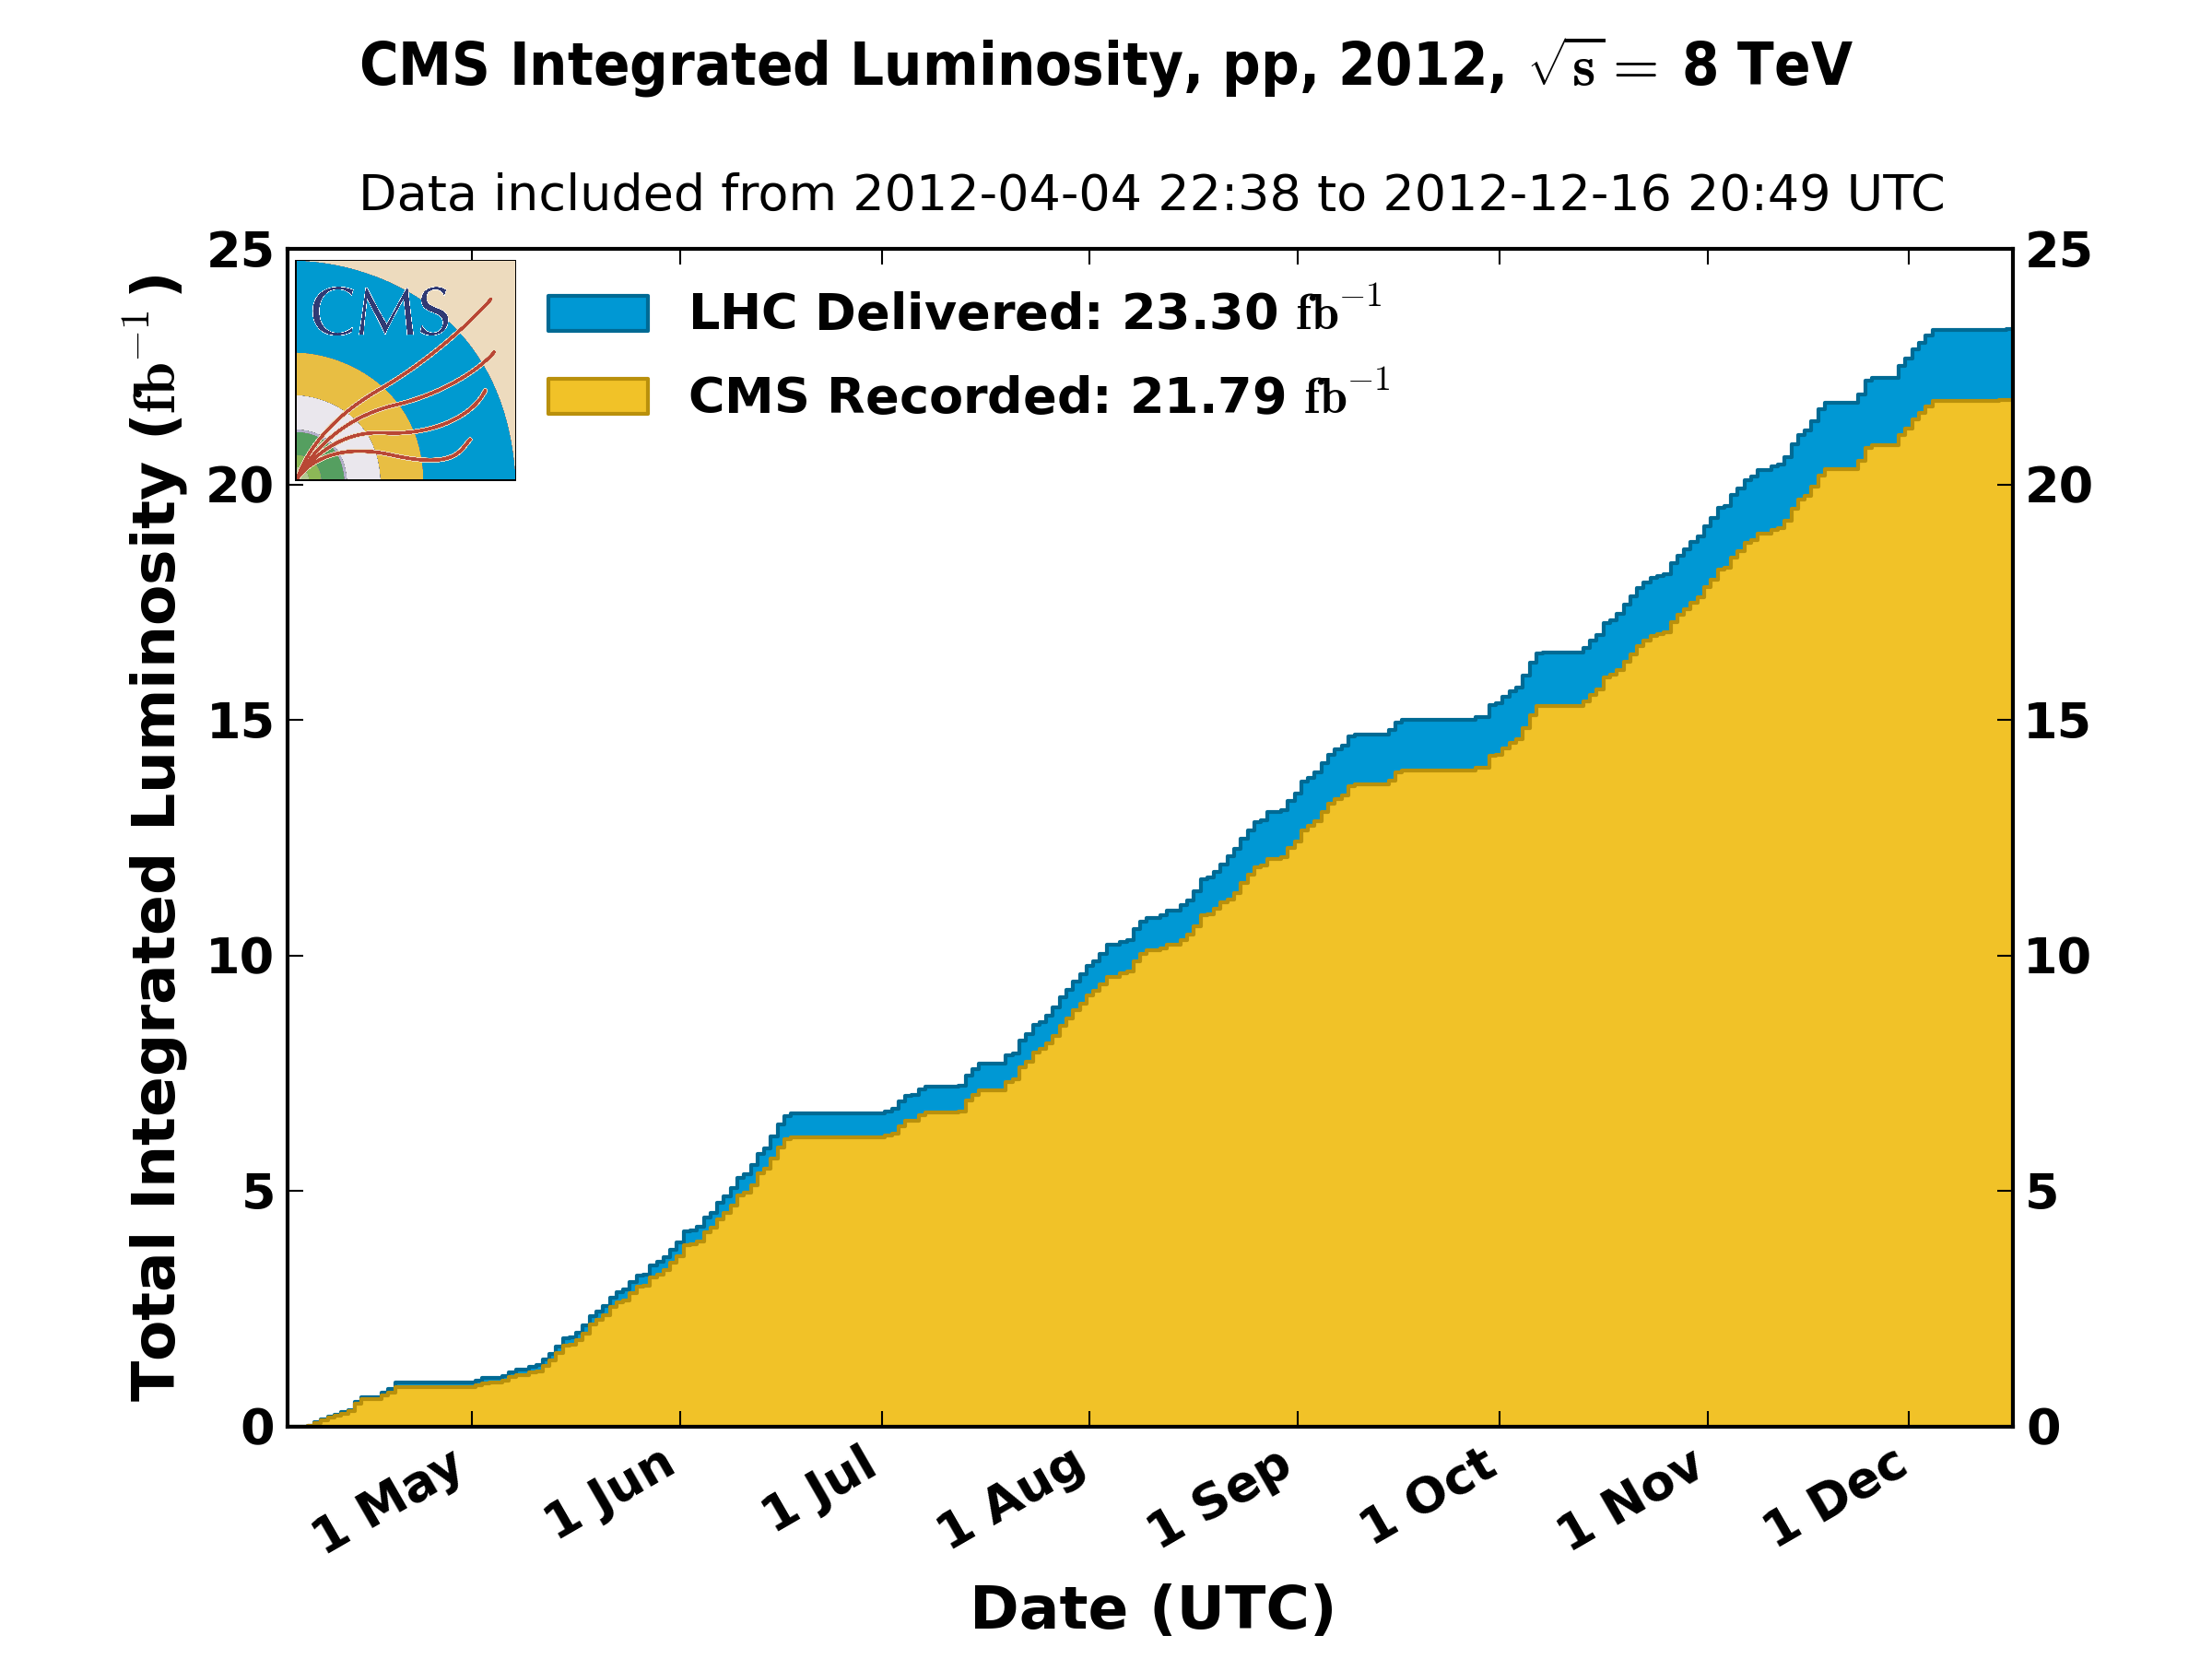
\includegraphics[scale=0.5]{Figures/int_lumi_per_day_cumulative_pp_2012.png} \\
       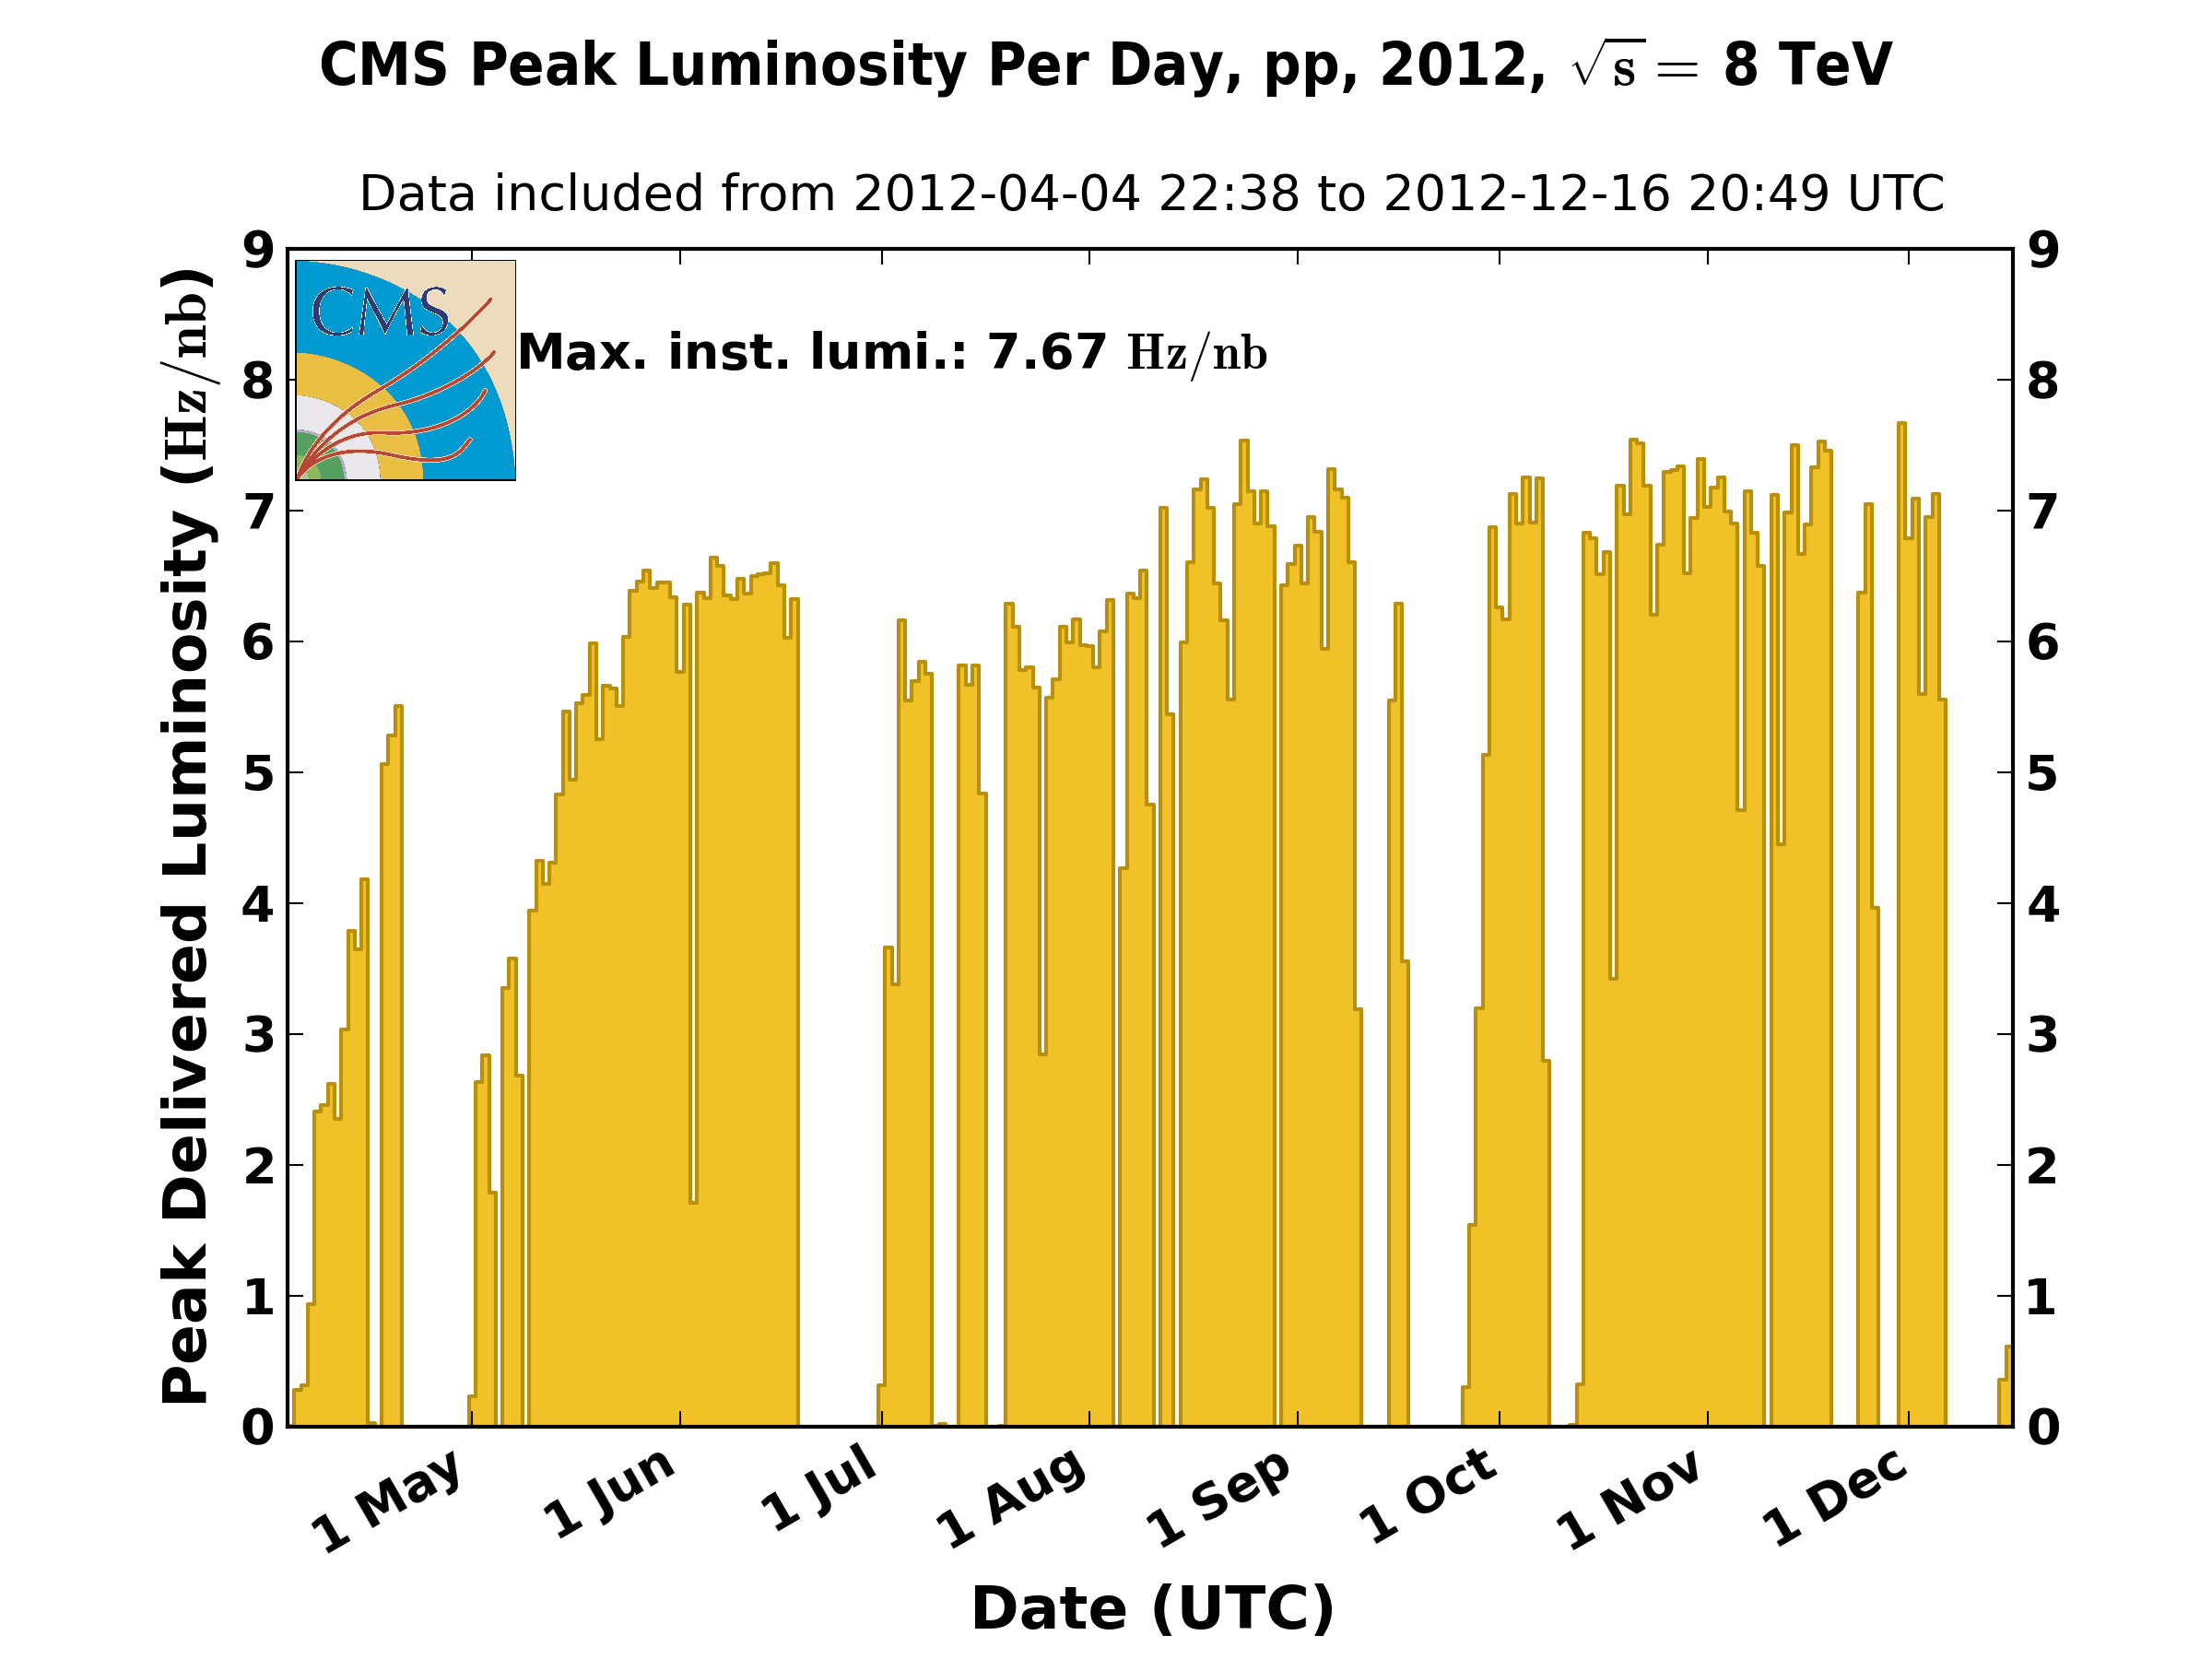
\includegraphics[scale=0.5]{Figures/peak_lumi_per_day_pp_2012.png} 
       \caption[Integrated and peak luminosity per day recorded by CMS in 2012.]{The integrated luminosity (top) delivered to and recorded by the CMS detector and the peak instantaneous luminosity (bottom) in 2012.}
\label{figapp:CMSLumi2012}
\end{figure}


\begin{figure}[!Hh]
       \centering
       \caption[Integrated and peak luminosity per day recorded by CMS in 2015.]{\textcolor{red}{FIXME: Add plots} The integrated luminosity (top) delivered to and recorded by the CMS detector and the peak instantaneous luminosity (bottom) in 2015 by \textcolor{red}{FIXME: Insert dates}.}
\label{figapp:CMSLumi2015}
\end{figure}



\subsection{Overview of the Detector}

The CMS detector is located at Point 5 on the LHC ring, approximately 100 m underground near the French village of Cessy, between Lake Geneva and the Jura mountain range.  It is designed to operate with pp collisions at $\sqrt{s} = 14$ TeV and a design luminosity of $10^{34}\text{ cm}^{-2}\text{s}^{-1}$.  With an expected proton-proton cross section of 100 mb at that design energy the event rate will be approximately $10^9$ inelastic events/s.  Computing limitations allow for approximately 100 events/s for storage and subsequent analysis so the online selection process (called the ``trigger'', discussed in Section~\ref{trigger}) must reduce this very large rate.  

The bunching of protons (within one bunch) and the short time between bunches, 25ns in 2015 and 50ns in 2012, result in the phenomeon called pileup in which multiple inelastic collisions are present in a single event.  The average number of collisions per bunch crossing measured in 2012 was 21, and in 2015 this value rose to \textcolor{red}{FIXME: put value}.  These so called pileup-distributions are shown in Figure~\ref{figapp:CMSpileup}.



\begin{figure}[!Hh]
       \centering
       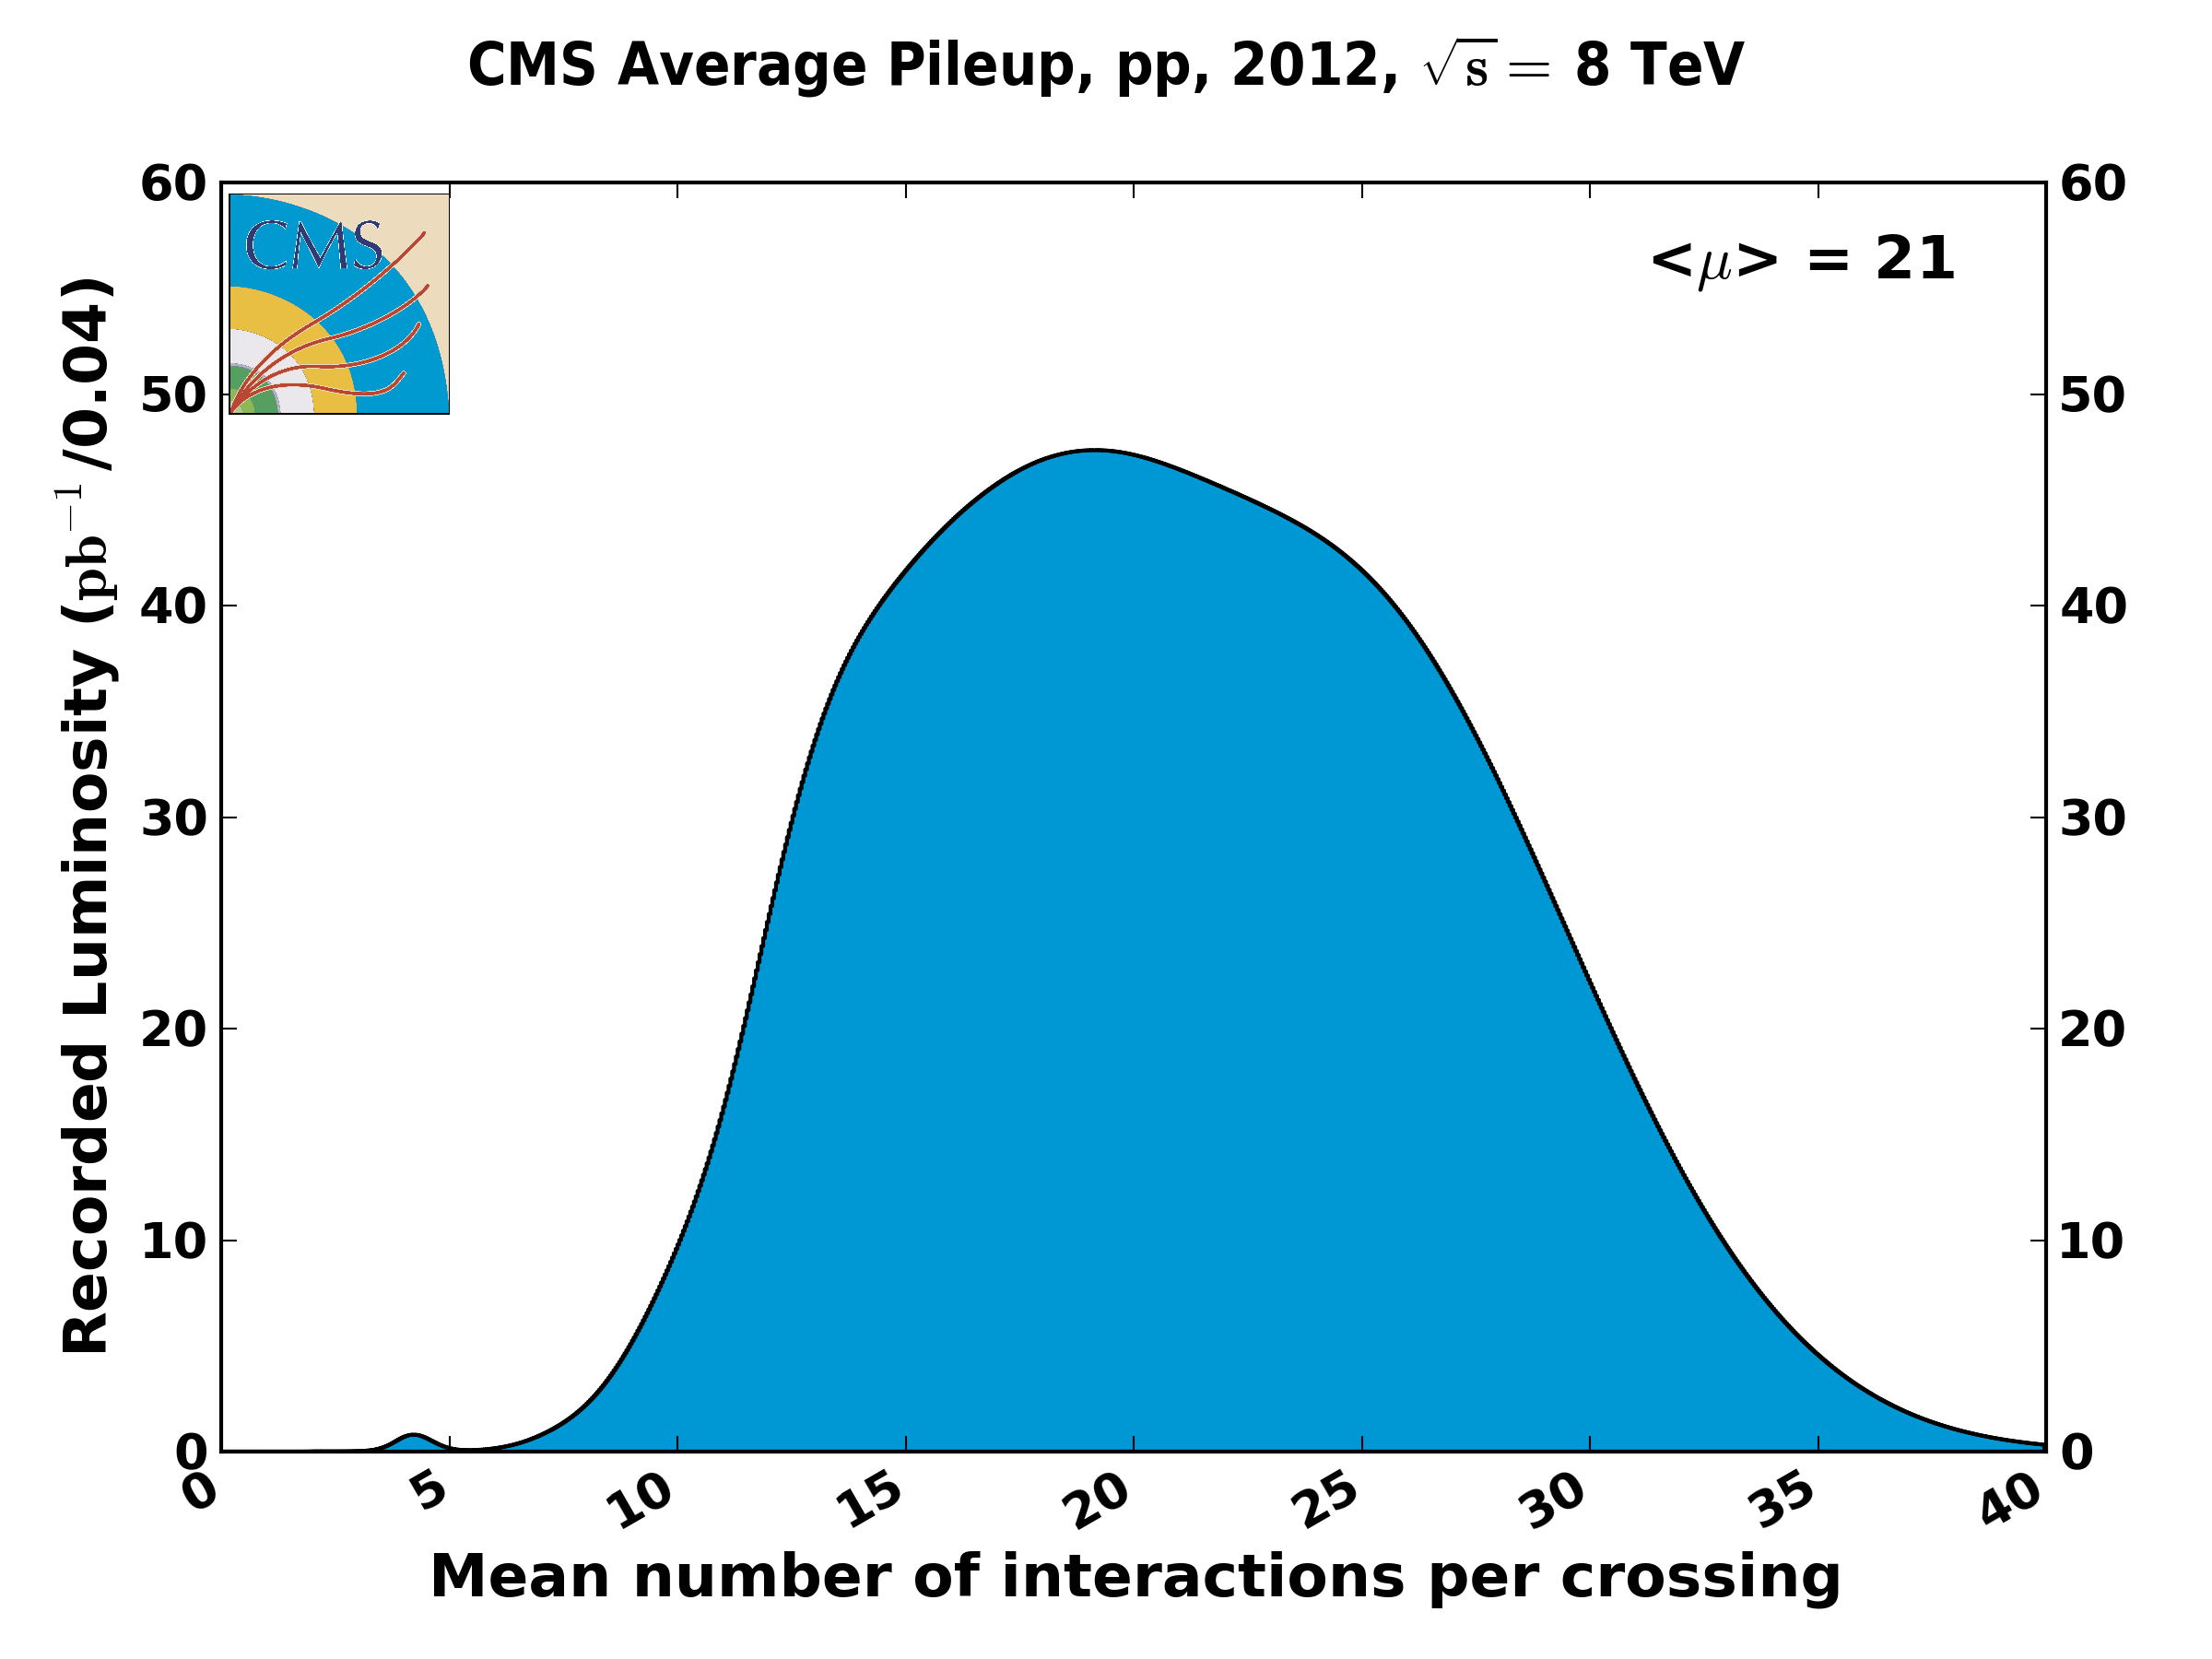
\includegraphics[scale=0.5]{Figures/pileup_pp_2012.png} \\
       \caption[Distribution of number of collisions per bunch crossing in 2012 and 2015.]{\textcolor{red}{FIXME: Add 2015 plot} The distribution of the number of interactions per event measured in 2012 (top) and 2015 (bottom).}
\label{figapp:CMSpileup}
\end{figure}

This results in a significant challenge to avoid confusing products from different interactions in the same collision, especially when response times from subdetectors can exceed the time between bunch crossings.  This effect is reduced in the CMS detector through the use of high-granulaty subdetectors with good time resolution that can achieve low occupancy.  This necessitates a very large number of detector channels, resulting in millions of total detector electronic channels that require good synchronization.  This provides the ability to determine which particles correspond to which event and which collision vertex within the event, and thus correspondingly the ability to accurately reconstruct the charges and momenta of the particles.  

The overall detector requirements for CMS are as follows:

\begin{itemize}

\item Muon systems:
  \begin{itemize}
  \item Good muon identification and momentum resolution for a wide range of momenta and angles
  \item Dimuon mass resolution of approximately one percent at 100 GeV (near the mass of the Z boson)
  \item Near perfect charge determination for muons with momenta less than 1 TeV
  \end{itemize}
\item Electromagnetic calorimeter:
  \begin{itemize}
  \item Good electromagnetic energy resolution
  \item Diphoton and Dielectron mass resolution of approximately one percent at 100 GeV
  \item Rejection of $\pi^0$ decays
  \item Efficient photon and lepton isolation at high luminosities
  \item Wide geometric coverage
  \end{itemize}
\item Inner Tracker:
  \begin{itemize}
  \item Good charged-particle momentum resolution and reconstruction efficiency
  \item Efficient triggering and offline tagging for $\tau$ leptons and jets from $b$-quark decays
  \end{itemize}
  
\item Hadronic calorimeter:
  \begin{itemize}
  \item Good missing-transverse-energy and dijet-mass resolution
  \item Large and hermetic geometric coverage and fine lateral segmentation (enabling the above point)
  \end{itemize}
\end{itemize}

The layout of the subsystems of CMS is shown in Figure~\ref{figapp:CMSlayout}.  Each is described in detail in sections \ref{solenoid} through \ref{muons}.



\begin{figure}[!Hh]
       \centering
       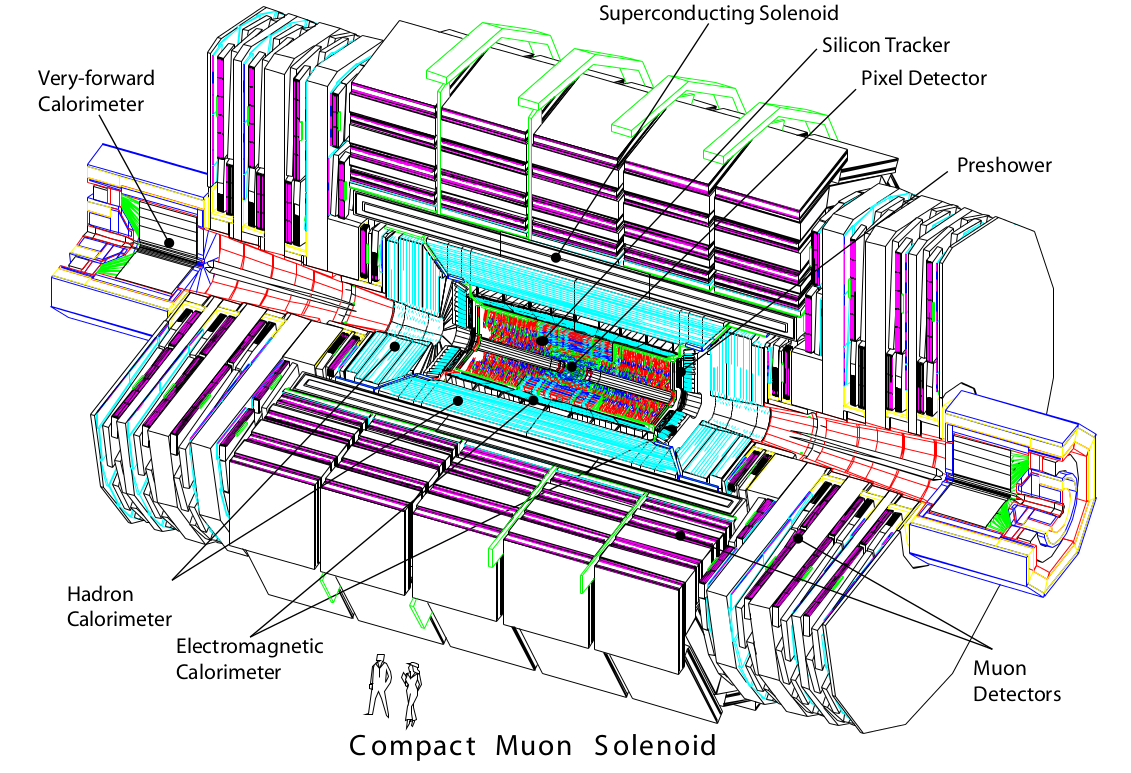
\includegraphics[scale=0.4]{Figures/CMSlayout.png} \\
       \caption[The basic layout of the CMS detector.]{A cutout diagram of the subsystems of the CMS detector, to scale.  The locations of the Solenoid magnet, Calorimeters, Trackers, and Muon Detectors are shown.  Figures of two people standing by the detector are given for a sense of size.}
\label{figapp:CMSlayout}
\end{figure}




\subsection{Conventions and Coordinates}

The convention for describing the geometry of the CMS detector is a right-handed coordinate system, defined with the origin at the nominal IP.  The z-axis points along the beam axis towards the Jura mountains from Point 5.  The y-axis points vertically upward and the x-axis points radially inward to the center of the LHC circle.  Thus the polar angle $\theta$ is taken from the z-axis and the azimuthal angle $\phi$ is measured from the x-axis in the x-y plane.  

Traditionally in collider physics the polar angle $\theta$ is not used, rather the psuedorapidity, $\eta$, is used.  Pseudorapidity is an approximation of the quantity called rapidity, $\varphi$, which is related to an object's speed.  Unlike speeds, at relativistic velocities rapidity is an additive quantity and the difference in rapidity between two particles ejected by a collision is invariant under Lorentz transfomations along the z-axis.  Also, production of particles tends to be close to uniform as a function of $\varphi$.  The rapidity, $\varphi$, is related to the Lorentz $\gamma$-factor as well as energy and momentum of a particle and is given by the expression:



\begin{equation}
\varphi = \cosh^{-1}(\gamma) = \tanh^{-1}\left(\frac{|\bold{p}|c}{E}\right) = \frac{1}{2}\ln\left( \frac{E+|\bold{p}|c}{E-|\bold{p}|c}\right).
\label{eq:rapidity_phi}
\end{equation}


Typically in colliders a version of the rapidity, y, is used that is defined only on the z-axis with respect to longitudinal momentum:

\begin{equation}
y \equiv  \frac{1}{2}\ln\left( \frac{E+p_Lc}{E-p_Lc}\right).
\label{eq:rapidity_y}
\end{equation}


In the limit where the particle's mass is negligible or where the particle is travelling close to the speed of light (applicable in the case of particles coming from collisions in the LHC) the rapidity is approximated by a simple function of the polar angle, $\theta$.  This value is called the psuedorapidity, $\eta$, and is given by the expression:


\begin{equation}
\eta \equiv  -\ln\left[ \tan\left(\frac{\theta}{2}\right)\right].
\label{eq:pseudorapidity}
\end{equation}

Both precision measurements and searches performed at the CMS experiment use kinematics defined in the transverse plane.  This is due to the fact that momentum in that plane can be determined to a high degree of accuracy and momentum conservation can be applied.  Also, like $\eta$, the transverse momentum ($p_T$) is invariant under longitudinal Lorentz transformations.  Thus $p_T$ and $\eta$ are the main kinematic variables used by most searches, including the search discussed in this thesis.  


\subsection{The Superconducting Solenoid}
\label{solenoid}

The superconducting magnet is designed to reach a field of 4 T in a free bore diameter of 6 m and length of 12.5 m, with a stored energy of 2.6 GJ at the full current.  The flux is returned via a 10,000 ton iron yoke which is comprised of five wheels and two endcaps composed of three disks each.  The solenoid itself has a 6.3 m cold bore and weighs 220 tons.  To achieve a 4 T field a very large number of ampere-turns is required (41.7 MA-turns) and the winding of the solenoid is composed of four layers.  This winding is composed of a stabilised and reinforced niobium-titanium (NbTi) conductor.

The ratio between the stored energy and cold mass of 220 t is very high, 11.6 KJ/kg, which results in a very significant mechanical deformation of 0.15\% during energising.  These values are much higher than other solenoidal detector magnets, a comparison of the stored energy and energy-over-mass ratios of the CMS magnet and other detector magnets is given in Figure~\ref{figapp:CMSstoredenergy}.  The main parameters of the CMS magnet are listed in Table~\ref{tab:CMSmagnetparams}.


\begin{figure}[!Hh]
       \centering
       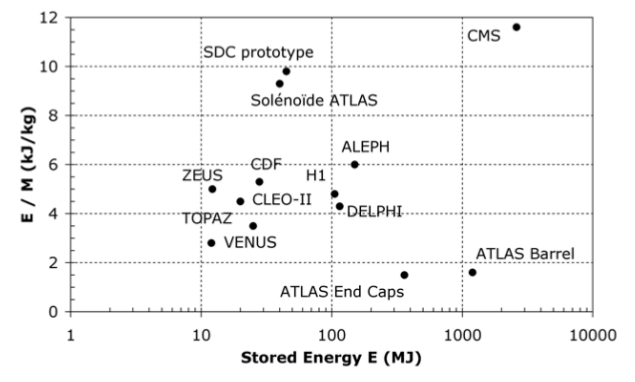
\includegraphics[scale=0.4]{Figures/CMSstoredenergy.png} \\
       \caption[The stored energy of CMS and other detector magnets.]{A comparison of the stored energy and energy-over-mass ratio E/M for CMS and other detector magnets~\cite{CMSdetector}.}
\label{figapp:CMSstoredenergy}
\end{figure}



\begin{table}[!Hhtbp]
\centering
\begin{tabular}{ll}
\hline
\hline
{General parameters} & {}\\
\hline
{Magnetic length} & {12.5 m}\\
{Cold bore diameter} & {6.3 m}\\
{Central magnetic induction} & {4 T}\\
{Total Ampere-turns} & {41.7 MA-turns}\\
{Nominal current} & {19.14 kA}\\
{Inductance} & {14.2 H}\\
{Stored energy} & {2.6 GJ}\\
\hline
\hline
{Cold mass} & {}\\
\hline
{Layout} & {Five modules mechanically and}\\
{} & {electrically coupled}\\
{Radial thickness of cold mass} & {312 mm}\\
{Radiation thickness of cold mass} & {3.9 $X_0$}\\
{Weight of cold mass} & {220 t}\\
{Maximum induction on conductor} & {4.6 T}\\
{Temperature margin w.r.t. operating temperature} & {1.8 K}\\
{Stored energy/unit cold mass} & {11.6 kJ/kg}\\
\hline
\hline
{Iron yoke} & {}\\
\hline
{Outer diameter of the iron flats} & {14 m}\\
{Length of barrel} & {13 m}\\
{Thickness of the iron layers in barrel} & {300, 630, and 630 mm}\\
{Mass of iron in barrel} & {6000 t}\\
{Thickness of iron disks in endcaps} & {250, 600, and 600 mm}\\
{Mass of iron in each endcap} & {2000 t}\\
{Total mass of iron in return yoke} & {10000 t}\\
\hline
\end{tabular}
\\
\caption[Parameters of the CMS magnet.]{The design parameters of the CMS magnet~\cite{CMSdetector}.}
\label{tab:CMSmagnetparams}
\end{table}

The purpose of the magnet is to provide a field that bends muon paths, allowing for precise momentum measurements.  In order to increase the longevity of the magnet, the decision to run it with a field of 3.8 T was made, which degraded the achievable muon momentum resolution by approximately 5\%~\cite{CMSperformance}.  The levels of the magnetic field and structure of the field lines can be seen in Figure~\ref{figapp:CMSfieldlines}, the return of the field the iron yoke is clearly visible.  



\begin{figure}[!Hh]
       \centering
       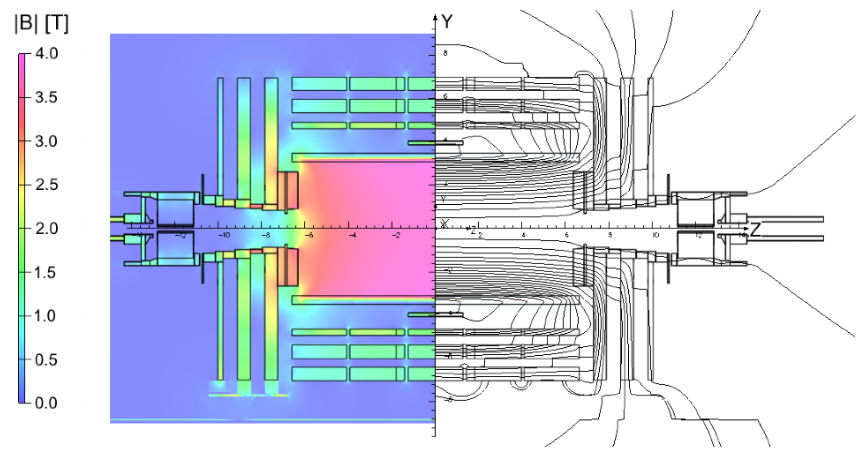
\includegraphics[scale=0.4]{Figures/CMSfieldlines.png} \\
       \caption[The values of the magnetic field and field lines of the CMS magnet in operation.]{A detailed map of the $|B|$ field (left) and the field lines (right) for a longitudinal section of CMS at a magnetic flux density of 3.8 T.  Each field line is an increment in magnetic flux of 6 Wb.~\cite{CMSperformance}.}
\label{figapp:CMSfieldlines}
\end{figure}

\subsection{The Silicon Tracker}
\label{tracker}

The innermost layer of the CMS detector is the inner tracking system, which is composed of an inner pixel tracker with 1440 modules and an outer strip tracker containing 15,148 strip modules.  With a total of approximately 200 $\text{m}^2$ of active silicon area the CMS inner tracker is the largest silicon tracker ever built~\cite{CMSdetector}.  At the LHC design luminosity there is an average of approximately 1000 particles expected per bunch crossing traversing the tracking system, from approximately 20 overlapping proton-proton interactions.  At a radius of 4 cm, the location of the innermost layer of the pixel tracker, this leads to a hit rate density of 1 MHz/$\text{mm}^2$.  In order to meet the resolution requirements the pixel size is $100 \times 150$ $\mu\text{m}^2$ in $r-\phi$ and $z$, respectively, which results in an occupancy of approximately $10^{-4}$ per pixel per LHC bunch crossing.  At the intermediate radii where larger strips ($10 \text{cm} \times 80 \mu\text{m}$) are located the occupancy is 2-3\% per strip and at the outer radii the cell sizes increase to $25 \text{cm} \times 180 \mu\text{m}$ and maintain an occupancy of apprixmately 1\%.  

The layout of the CMS tracker is given in Figure~\ref{figapp:TrackerLayout} and is composed of 4 major component systems.  The innermost system is the pixel detector (PIXEL), composed of three cylindrical layers in the barrel (BPix) located at radii of 4.4, 7.3, and 10.2 cm and two endcap disks (FPix) located at $z=\pm34.5$ and $z=\pm46.5$ cm.  In total the PIXEL system covers an area of approximately 1 $\text{m}^2$ and is composed of 66 million pixels.  The pixel detector covers a pseudorapidity range of $|\eta| < 2.5$, matching the acceptance of the central tracker.  The layout of the pixel detector and its hit coverage is given in Figure~\ref{figapp:PixelCoverage}.


\begin{figure}[!Hh]
       \centering
       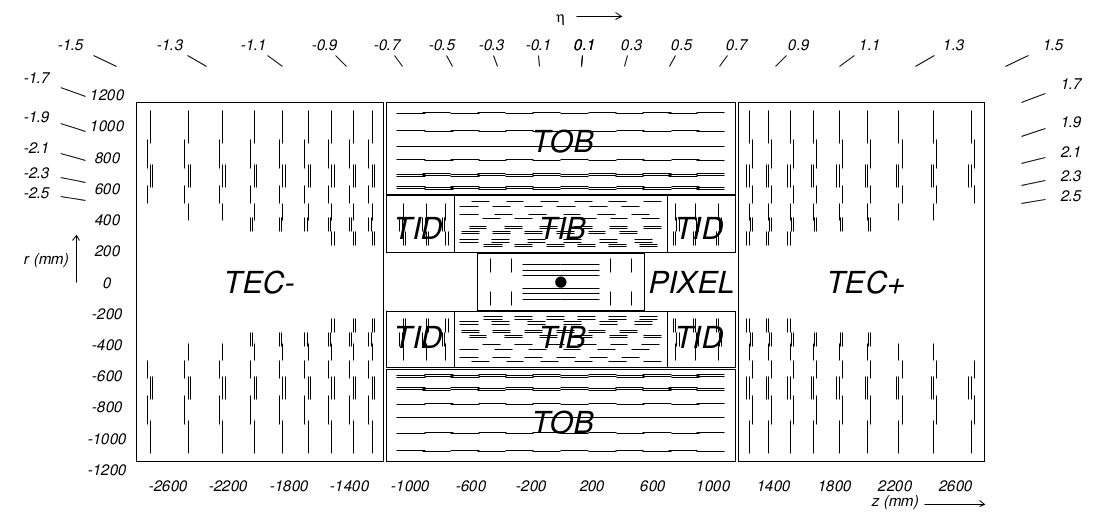
\includegraphics[scale=0.4]{Figures/TrackerLayout.png} \\
       \caption[The longitudinal cross section of the layout of the CMS tracker.]{The longitudinal cross section of the layout of the CMS tracker~\cite{CMSdetector}.  Each line represents a module, with double lines indicating back-to-back modules that deliver stereo hits.}
\label{figapp:TrackerLayout}
\end{figure}


\begin{figure}[!Hh]
       \centering
       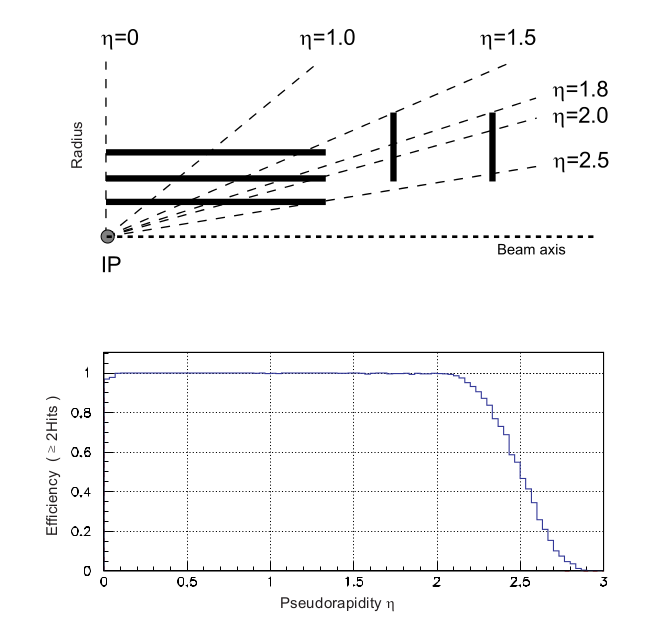
\includegraphics[scale=0.6]{Figures/PixelCoverage.png} \\
       \caption[The layout of the pixel detector.]{The geometrical layout of the pixel detector (top) and the hit coverage with respect to pseudorapidity (bottom)~\cite{CMSdetector}.}
\label{figapp:PixelCoverage}
\end{figure}


The other three systems compose the strip tracker and are located at radii from 20 cm to 116 cm.  The Tracker Inner Barrel and Inner Disks (TIB/TID) are composed of 4 barrel layers supplemented by 3 encdcap disks at each end, covering a radius up to 55 cm.  Thus the TIB/TID delivers up to 4 $r-\phi$ measurements per trajectory.  It uses 320 $\mu\text{m}$ thick silicon micro-strip sensors oriented parallel to the beam axis in the barrel and perpendicular to it in the endcaps.  The strip pitch (inter-strip distance) is 80 $\mu\text{m}$  on layers 1 and 2 and 120 $\mu\text{m}$ on layers 3 and 4 of the TIB, varying from 100 $\mu\text{m}$ to 141 $\mu\text{m}$  in the TID.  The strip pitch, width, and length are chosen to minimize inter-strip capacitance which in turn optimizes the resolution and occupancy as well as ensuring high voltage operational stability~\cite{STRIPtracker}.  The TIB/TID is in turn surrounded by the Tracker Outer Barrel (TOB) which consists of 6 barrel layers of 500 $\mu\text{m}$ thick sensors extending to a radius of 116 cm.  The strip pitches are 183 $\mu\text{m}$ on the first 4 layers and 122 $\mu\text{m}$ on the last 2 layers.  The TOB extends in $z$ between $\pm118$ cm and beyond it lie the Tracker EndCaps (TEC).  Each TEC consists of 9 disks covering $124\text{cm} < |z| < 282 \text{cm}$ and $22.5\text{cm} < |z| < 113.5\text{cm}$.  There are 4 inner rings with 320 $\mu\text{m}$ thick strips and 5 outer rings with 500 $\mu\text{m}$ thick strips, averaging pitches ranging from 97 $\mu\text{m}$ to 184 $\mu\text{m}$.  

In addition to the modules listed above, the first two layers and rings of the TIB, TID, and TOB as well as rings 1, 2, and 5 of the TECs contain a second micro-strip module mounted back-to-back with a stereo angle of 100 mrad which provides a measurement in the second coordinate ($z$ in the case of the barrel, $r$ in the case of the disks).  The strip tracker layout in total assures at least approximately 9 hits in the $|\eta| < 2.4$ range, 4 of which are two-dimensional measurements.  The complete coverage of the strip tracker ends at $|\eta| = 2.5$, the overall number of measurment points in the strip tracker is given as a function of $\eta$ in Figure~\ref{figapp:StripCoverage}.


\begin{figure}[!Hh]
       \centering
       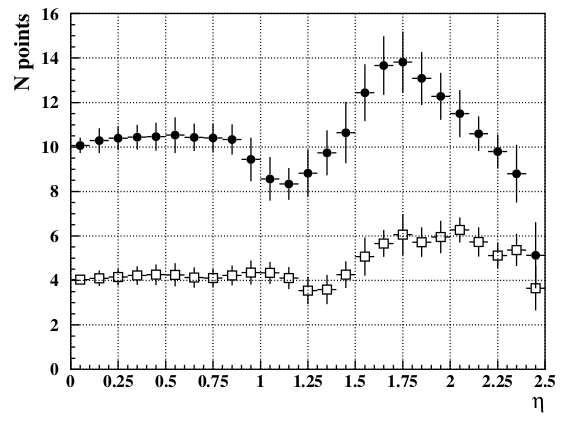
\includegraphics[scale=0.6]{Figures/StripCoverage.png} \\
       \caption[The coverage of the strip tracker.]{The number of measurment points in the strip tracker with respect to $\eta$, black circles represent the total number while white squares represent stereo layers~\cite{CMSdetector}.}
\label{figapp:StripCoverage}
\end{figure}


The pixel and strip detector modules performed very well in Run I (in 2011 and 2012), the hit efficiencies are shown in Figure~\ref{figapp:TrackerHitEfficiency}.  The tracker allows for accurate reconstruction of charged particle tracks as well as high-resolution measurements of the interaction vertices, which are both described in detail in Section~\ref{trackreco}.  


\begin{figure}[!Hh]
       \centering
       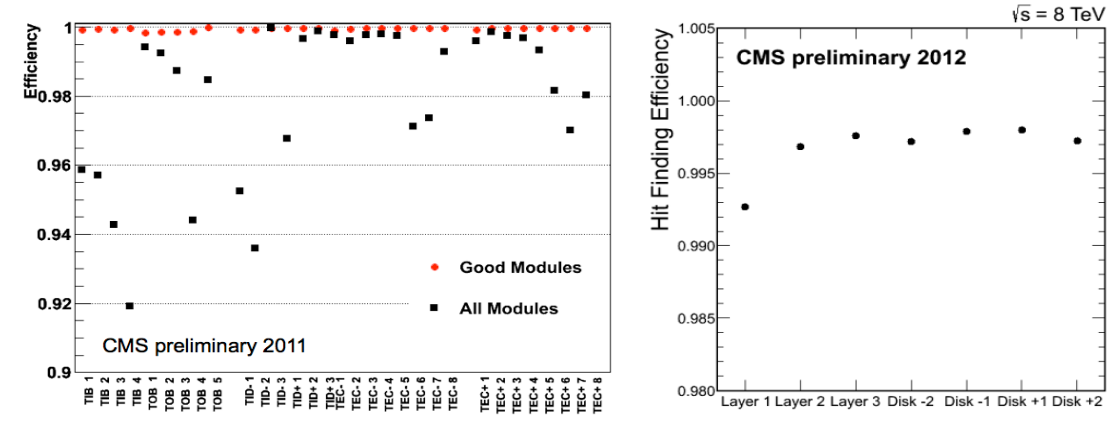
\includegraphics[scale=0.4]{Figures/TrackerHitEfficiency.png} \\
       \caption[The hit efficiency of the CMS tracker.]{The single hit efficiency of the strip (left) and pixel (right) trackers~\cite{STRIPtracker}.  Only the good (fully operational) modules were considered for the pixels.}
\label{figapp:TrackerHitEfficiency}
\end{figure}


\subsection{The Electromagnetic Calorimeter}
\label{ecal}

The electromagnetic calorimeter (ECAL) immediately surrounds the silicon tracker.  The ECAL is a hermetic and homogeneous calorimeter which is composed of 75,848 lead tungstate ($\text{PbWO}_4$) crystals in total, with 61,200 located in the central barrel section and 7,324 in each endcap.  A preshower detector is located in front of the endcap crystals, which serves to identify neutral pions in the endcaps and help electron identification against minimum ionizing particles~\cite{CMStdr}.  


The barrel portion of the ECAL (EB) covers a pseudorapidity range of $|\eta| < 1.479$ with an inner radius of 1.29 m.  The granularity is 360-fold in the $\phi$-direction, and (2$\times$85)-fold in $\eta$, resulting in the total of 61,200 individual crystals.  The crystals themselves are tapered in shape, slightly varying with position in $\eta$.  The endcap portion (EE) covers a pseudorapidity range of $1.479 < |\eta| < 3.0$, with a longitudinal distance from the inner surface to the interaction point of 315.4 cm.  The preshower detector (ES) sits directly in front of each EB, covering a pseudorapidity range of $1.653 < |\eta| < 2.6$. The overall layout of the ECAL is given in Figure~\ref{figapp:ECALlayout}.  




\begin{figure}[!Hh]
       \centering
       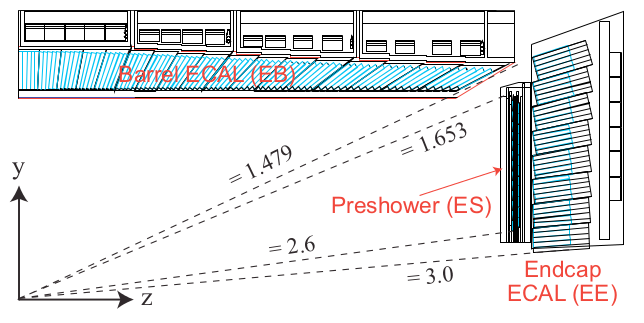
\includegraphics[scale=0.6]{Figures/ECALlayout.png} \\
       \caption[The layout of the CMS electromagnetic calorimeter.]{The layout of the ECAL, showing the Barrel ECAL (EB), Endcap ECAL (EE), and Preshower ECAL (ES)~\cite{CMStdr}.  The dashed lines are labeled with pseudorapidity values for reference.}
\label{figapp:ECALlayout}
\end{figure}


A driving criterion in the design of the ECAL was the ability to detect decays to two photons, a main decay mode of the Higgs boson.  The characteristics of the $\text{PbWO}_4$ crystals made them an appropriate choice to help meet this criterion.  The density (8.28 g/$\text{cm}^3$) and short radiation length of 0.89 cm (defined as the mean path length over which a relativistic particle loses energy by a factor of $1/e$) allows for a compact design.  The small Moli$\grave{\text{e}}$re radius of 2.2 cm (the radius of a cylinder transverse to a charged particle's direction of flight in which on average at least 90\% of the particle's energy is deposited) provides a fine granularity.  Additionally, in the years leading up to the construction of the LHC, $\text{PbWO}_4$ crystal production improved, becoming capable of producing optically clear and radiation-hard crystals.  The scintillation decay time of the $\text{PbWO}_4$ crystals in the ECAL is on the same order as the LHC design bunch crossing time, approximately 80\% of the light is emitted in 25 ns.  At the design operation temperature of $18^{\circ}$ C the light output is approximately 4.5 photoelectrons per MeV.  The scintillated light is blue-green in color, with a broad maximum wavelength of 420-430 nm~\cite{CMSdetector}.

The scintillated light is collected by photodetectors located at the end of each crystal.  In the barrel, avalanche photodiodes (APDs) that are specially produced for the CMS ECAL are used.  Two are placed on the backs of each crystal module.  In the endcap, the photodetectors used are vacuum phototriodes (VPTs), also specially produced for the ECAL, with one per crystal module.  ECAL modules of both the endcap and the barrel are shown with their attached photodetectors in Figure~\ref{figapp:ECALphotodetectors}.

\begin{figure}[!Hh]
       \centering
       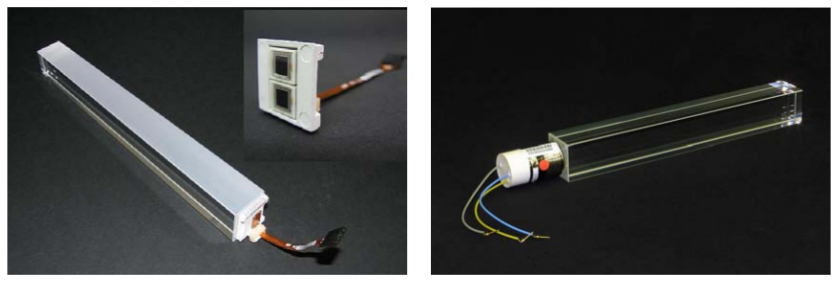
\includegraphics[scale=0.5]{Figures/ECALphotodetectors.png} \\
       \caption[Photodetectors and crystal modules in the CMS eletromagnetic calorimeter.]{$\text{PbWO}_4$ crystals with their photodetectors attached~\cite{CMStdr}.  A barrel crystal with attached APD (left), detached pair of APDs (left insert), and endcap crystal with VPT attached (right).}
\label{figapp:ECALphotodetectors}
\end{figure}

The APDs and VPTs are fast and radiation hard and are able to operate in a 4-T magnetic field.  The $\text{PbWO}_4$ crystals output a relatively small amount of light, so both photodetector types must have strong amplification.  The APDs operate at a gain of 50 and cover an active area of 25 $\text{mm}^2$.  The VPTs, of which there are only one per crystal, operate at a mean gain of 10.2 in a zero field and cover an active area of approximately 280 $\text{mm}^2$.  When the VPTs are placed in a strong axial magnetic field the response is slightly reduced, and there is a variation of response with the angle of the VPT axis with respect to the field.  The mean response in a 4-T field is typically at least 90\% of that in a zero magnetic field.  Both the APDs and VPTs were tested and screened to ensure reliable operation for 10 years under the high luminosity LHC conditions.



\subsection{The Hadronic Calorimeter}
\label{hcal}


The hadronic calorimeter (HCAL) is located directly outside of the ECAL and its role is to measure the energies of hadron jets and to help infer the missing transverse energy in an event that may result from neutrinos and/or exotic particles.  The HCAL is composed of 4 main components: the barrel (HB), the endcap (HE), the outer (HO), and the forward (HF) calorimeters.  Each subcomponent is a sampling calorimeter using the well known calorimetry strategy of tile and wavelength shifting fibers~\cite{CMSdetector}.  The layout of these subsystems are given in Figure~\ref{figapp:HCALlayout}.


\begin{figure}[!Hh]
%       \centering
       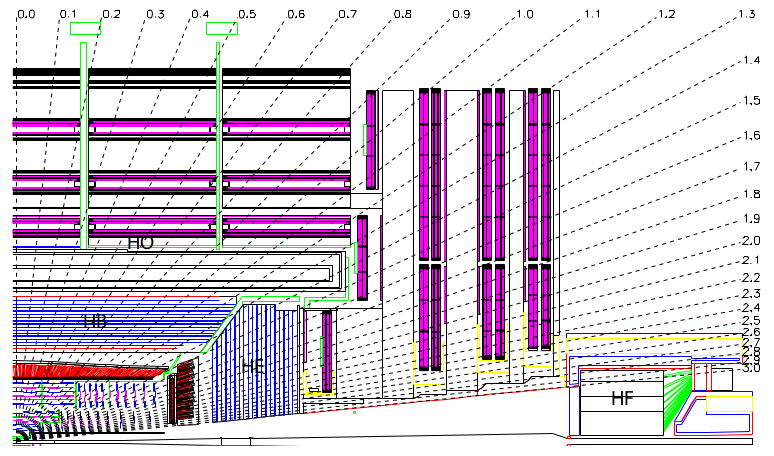
\includegraphics[scale=0.6]{Figures/HCALlayout.png} \\
       \caption[Layout of the CMS hadronic calorimeter.]{A longitudinal cross section of the layout of the CMS detector featuring the locations of the hadronic calorimeter: the barrel (HB), the endcap (HE), the outer HCAL (HO), and the forward HCAL (HF)~\cite{CMSdetector}.}
\label{figapp:HCALlayout}
\end{figure}

The HB inner radius is restricted by the outer edge of the ECAL, $R=1.77$ m, and the inner edge of the magnet coil, $R=2.95$ m.  It is composed of 36 identical azimuthal wedges which form each of two half barrels (HB+ and HB-), together covering the pseudorapidity range of $|\eta| < 1.3$.  Each wedge is is segmented azimuthally is segmented in to 4 sectors and is composed of brass absorber plates that are bolted together in a staggered fashion as to produce a configuration which contains no projective dead material for the full extent of the wedge.  For structural integrity the brass absorbers are reinforced by steel plates on the front and back of the wedges.  The scintillator, which is made of plastic, is divided into 16 $\eta$ sectors producing a segmentation of $(\Delta\eta,\Delta\phi) = (0.087, 0.087)$.  The light from the scintillators is brought out by wavelength shifting fibers and after exiting the scintillator the fibers are spliced to clear fibers.  These clear fibers bring the light to the hybrid photodiode for eventual data collecting.  

The HE cover a large portion of the pseudorapidity range, $1.3 < |\eta| < 3$, which is a region containing approximately 34\% of final state particles.  Because the HE is inserted into the end of a high T solenoidal magnet, the absorber had to be composed of a non-magnetic material.  In order to simultaneously satisfy that condition and others such as a maximum number of interaction lengths to contain hadronic showers, C26000 cartridge brass was used~\cite{CMSdetector}.  As with the HB, the HE absorbers are staggered to avoid creation of any projective dead material.  In addition, they are shaped to minimize any cracks between HB and HE, rather than being shaped to optimize single-particle energy resolution.  This is due to the fact that jet resolution in the HE is limited by pileup, magnetic effects, and parton fragmentation in any case.  Also as with the HB, the HE contain scintillators whose light is brought out via wavelenth shifting fibers to photodetectors and readout electronics.  

Between the electronic and hadronic barrel calorimeters (EB and HB) there is not enough stopping power in the central pseudorapidity region to provide adequate containment for hadronic showers.  Thus, to ensure that there is sufficent sampling depth for tha tregion, the HCAL is extended outside the solenoid with the HO, also called a tail catcher.  The HO uses the solenoid coil as an extra absorber and is used to identify showers that start late and to measure any additional shower energy deposited after the HB.  The HO is placed as the first sensitive layer in each of the five rings of the iron yoke (2.536 m wide along the z-axis).  It is segmented in to 12 identical azimuthal sectors, closely matching the geometry of the barrel muon system.  Together with the HE and the HB the HO is segmented in the $r,z$ plane according to Figure~\ref{figapp:HCALsegmentation}.  



\begin{figure}[!Hh]
%       \centering
       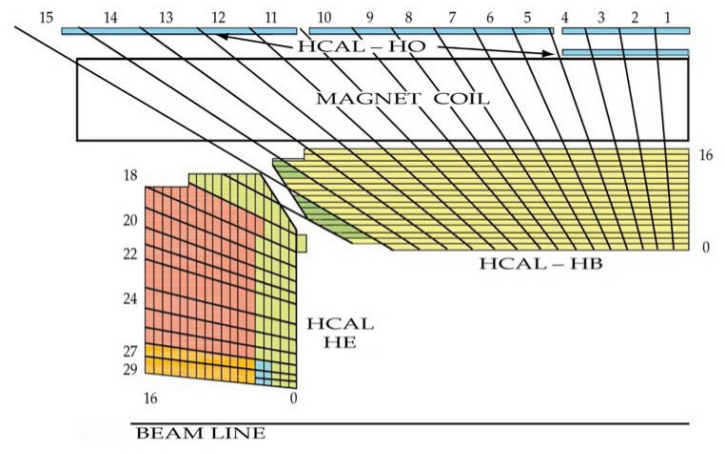
\includegraphics[scale=0.6]{Figures/HCALsegmentation.png} \\
       \caption[Segmentation of the CMS hadronic calorimeter.]{A cross section in the $r,z$ plane of the segmentation of the HB, HE, and HO~\cite{CMSdetector}.}
\label{figapp:HCALsegmentation}
\end{figure}

The HF is located in a region that experiences huge particle fluxes, the front face is located 11.2 m from the interaction point, with an inner radius of 12.5 cm and an outer radius of 130 cm.  It receives on average 760 GeV per proton-proton interaction as opposed to 100 GeV for the rest of the detector.  To cope with this environment the HF is housed in a hermetic radiation shield which consists of layers of 40 cm thick steel, 40 cm of concrete, and 5 cm of polyethylene.  Additionally, the active elements of the HF are radiation-hard quartz fibers.  The calorimeter itself is subdivided into two segments longitudinally, one which runs the full depth of the detector and one which only starts at a depth of 22 cm from the front,  which are read out separately.  This allows the HF to distinguish between showers generated by electrons and photons, which deposit a majority of their energy in the first 22 cm, from hadronic showers which deposit their energy roughly equally throughout the calorimeter.



\subsection{The Muon system}
\label{muons}

Precision measurement of muons is of critical importance, as many final state decays of exotic processes and signatures of supersymmetry include one or more muon muons, and the ``gold plated'' SM Higgs decay mode of $h \rightarrow ZZ \rightarrow 4 \mu$ (as well as a few other Higgs decay modes) produces many muons in its decay states.  Muon final states possess great discovery potential, as final states in which all leptons are muons are less affected by radiative losses in the tracker system.  Thus, as indicated by the experiment's middle initial, muon detection is a main role that the CMS detector must perform well.  The combined muon system has three functions: muon identification, momentum measurement, and triggering.  Good muon momentum resolutions and trigger capability are facilitated by the high-field solenoid magnet and the flux-return yoke.  The yoke also serves to absorb hadrons to assist with muon identification.

The muon system has the capability to reconstruct muon momentum and charge over the entire kinematic range of the LHC, and is composed of 3 separate types of gaseous particle detectors.  As with the calorimeters, the muon system is composed of a cylindrical barrel section and two planar endcap sections.  The eventual background rates the muon system was uncertain during construction, and the ability of the muon system to correctly measure the beam-crossing time at full LHC luminosity, so a dedicated trigger system was added in both the barrel and endcap sections.  This system, consisting of Resistive Plate Chambers (RPC) provides a fast and fully independent trigger with a sharp $p_T$ threshold over a large pseudorapidity range, $|\eta|< 1.6$.  In the barrel, where the overall muon rate and neutron-induced background is low, and the 4-T magnetic field is low as well, so drift chambers with rectangular drift cells are used.  This system, the Drift Tubes (DT), covers a pseudorapidity range of $|\eta| < 1.2$.  In the endcap regions the muon and background rates are high, and the magnetic field is large and non-uniform, so Cathode Strip Chambers (CSC) are used because of their fast response time, fine segmentation, and radation-hardness.  The CSCs cover a pseudorapidity range of $0.9 < |\eta| < 2.4$.  The layout of these three systems is shown in a quadrant cutout of the CMS detector shown in Figure~\ref{figapp:Muoncutout}.





\begin{figure}[!Hh]
%       \centering
       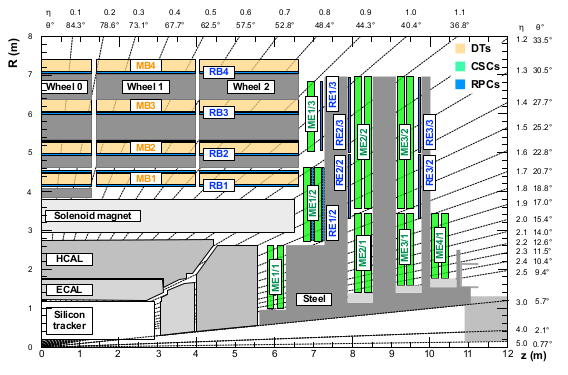
\includegraphics[scale=0.8]{Figures/Muoncutout.png} \\
       \caption[The layout of the CMS muon system.]{The cross section of a quadrant of the CMS detector, in the $R-z$ plane~\cite{CMSperformance}.  The muon systems are featured, the four DT stations (light orange) are labeled MB, the CSCs (green) are labeled ME, and the RPCs (blue) which are in both barrel and endcap are labeled both MB and ME, respectively.  MB stands for ``muon barrel'' and ME for ``muon endcap''.  The dark gray regions represent the steel disks.}
\label{figapp:Muoncutout}
\end{figure}


\subsubsection{The Resistive Plate Chamber system}
\label{rpcs}

The RPCs are gaseous parallel-plate detectors that provide a time resolution comparable to that of scintillators.  An RPC is capable of identifying the time of an ionising event in a significantly shorter time than the 25ns between two consective LHC bunch crossings.  A muon trigger based on RPCs can identify the bunch crossing to which a muon track is associated unambiguously, and thus the RPCs are a detector system dedicated to triggering.  The RPCs cover a pseudorapidity of $|\eta| < 1.6$ which covers the entire range of the DTs and a portion of the range of the CSCs.  

The RPCs are double-gap (called ``up'' and ``down'' gaps) gaseous detectors, operated in avalanch mode with common pick-up read-out strips located between the two gaps.  Each gap consists of a pair of 2 mm thick bakelite plates coated in a thin graphite layer encapsulating the gap which is filled by gas mixture of 95.2\% Freon, 4.5\% isobutane, and 0.3\% sulphur hexaflouride.  The plates are held to a voltage of 9.6 kV, and muons that traverse the gas ionize an atom in the gas, causing an avalanch which induces a charge that is readout by the on-board electronics.  

The RPCs are partioned in the $\eta$-direction, in two and three partitions (called rolls) in the barrel and endcap, respectively.  The layout of a typical barrel RPC is shown in Figure~\ref{figapp:RPClayout}.  The RPCs are arranged in stations following a similar sequence to the DTs and RPCs.  The RPC barrel (RB) has 4 stations, RB1-4, while the RPC endcap (RE) has 3 stations, RE1-3, totalling 480 chambers overall.  



\begin{figure}[!Hh]
%       \centering
       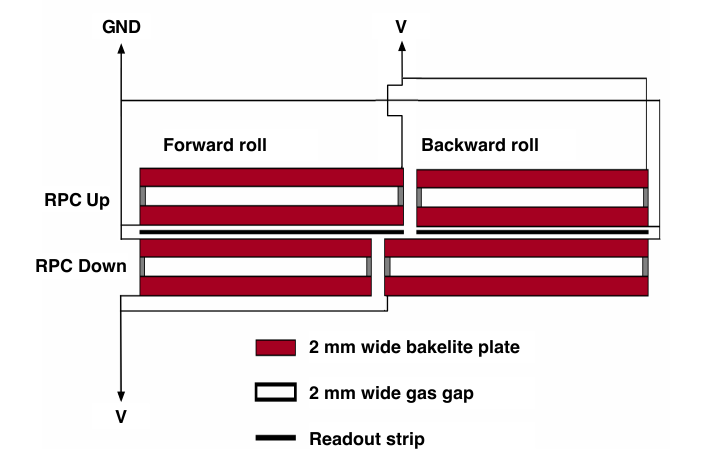
\includegraphics[scale=0.6]{Figures/RPClayout.png} \\
       \caption[The layout of a resistive plate chamber.]{A schematic of a barrel RPC with two partitions (rolls)~\cite{CMSperformance}.}
\label{figapp:RPClayout}
\end{figure}



\subsubsection{The Drift Tube system}
\label{dts}

The DTs are located in the barrel, covering a pseudorapidity range of $|\eta < 1.2|$.  In this region the muon rate is low, the neutron background is small (except for at the outermost layer of the DTs), and the magnetic field is predominantly uniform with a strength of 0.4 T and lower~\cite{CMSperformance}.  Thus drift chambers are used with rectangular cells and electrical field shaping implemented.  There are four stations in the barrel, labeled MB1-4, which are divided into 12 $\phi$-segments.  

The DTs contain basic elements called drift cells, with a transverse area of $42 \times 13 \text{mm}^2$ and a 50 $\mu$m diameter gold-plated anode wire at the center.  A voltage of 3600 V is applied to the wire, and 4 electrodes are used (including 2 cathode strips) to shape the drift field: 2 on the ground planes between layers and 2 on the side walls of the tube.  These electrodes are held at 1800 and -1200 V, respectively.  The layout of the drift cell with the drift paths and an example incident muon path is depicted in Figure~\ref{figapp:DTlayout}.



\begin{figure}[!Hh]
%       \centering
       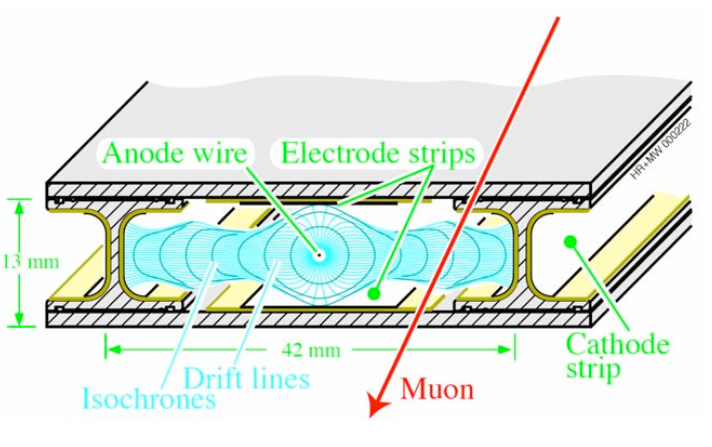
\includegraphics[scale=0.6]{Figures/DTlayout.png} \\
       \caption[The layout of drift cell of the drift tube system.]{A schematic of a drift cell, shown with the drift lines and an example incident muon path~\cite{CMSdetector}.}
\label{figapp:DTlayout}
\end{figure}

The gas mixture which is ionized by incident muons is an 85\%/15\% blend of argon (Ar) and carbon dioxide (CO$_2$).  This provides good quenching properties, as well as a saturated drift velocity of approximately 55 $\mu$m/ns and a maximum drift time of 400 ns.  These drift cells are staggered, with four layers of parallel cells forming a superlayer (SL).  Each DT chamber consists of 2 SLs that measure the $r-\phi$ coordinates and one orthogonal SL that measures the $r-z$ coordinate (except for the outermost layer of DTs, MB4, which only has an $r-\phi$ layer).  



\subsubsection{The Cathode Strip Chamber system}
\label{cscs}



The CSCs cover a pseudorapidity range of $1.2 < |\eta| < 2.4$, and consist of a total of 473 chambers in the first LHC run.  There are 108 in the first station (ME1), 54 in the second and third (ME2 and ME3), and 18 in the inner ring of the outermost station (ME4), as depicted in Figure~\ref{figapp:Muoncutout}.  On one side of the CMS detector, 5 CSCs were placed in an outer ring on the 4th station (ME4/2), and these were expanded to the full 18 per endcap in the second LHC run.  

CSCs are trapezoidal in shape and cover either $10^\circ$ or $20^\circ$ in $\phi$.  All except for ME1/3 overlap and provide continuous $\phi$-coverage.  They aare comprised of 6 anode wire planes interspersed with 7 cathode panels.  The wires run azimuthally and define the radial coordinate of a track.  The strips are milled directly on to the cathode panels and run lengthwise at a constant width in $\Delta\phi$.  While there are varying total sizes of chambers, the largest ones (ME2/2 and ME3/2) are approximately $3.4 \times 1.5 \text{ m}^2$ in size, and a sample schematic layout of a typical CSC is given in Figure~\ref{figapp:CSClayout}.




\begin{figure}[!Hh]
       \centering
       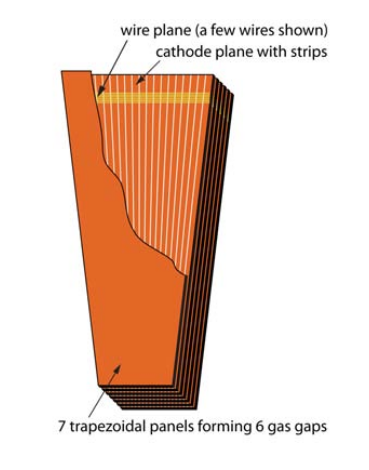
\includegraphics[scale=0.8]{Figures/CSClayout.png} \\
       \caption[The layout of a cathode strip chamber.]{A schematic of a CSC, shown with all six layers~\cite{CMSdetector}.}
\label{figapp:CSClayout}
\end{figure}



The nominal gas mixture used in the CSCs for ionization is 40\% Ar, 50\% $\text{CO}_2$, and 10\% $\text{CF}_4$.  The primary role of the $\text{CO}_2$ is as a non-flammable quencher for achieving large gas gains, and the role of the $\text{CF}_4$ is to prevent polymerization on the anode wires.  The nominal operating voltage was chosen to be 3.6kV which corresponds to a gas gain on the order of $7 \times 10^4$, except for the inner stations (ME1), for which 3.3kV was chosen.  These voltages provide very high efficiencies with an adequate signal-to-noise ratio.  

Each chamber has a set of anode front end boards (AFEBs) that are amplifier-discriminators and serve to initially shape and read out charge avalanches from incident muons ionizing the gas.  All the AFEBs send their output to an FPGA-based anode local charged track (ALCT) board, of which there is one per chamber.  The ALCT checks every bunch crossing for patterns in the 6 planes that are consisent with a muon track originating from the interaction point.  Any pattern that is found is called an ALCT, and serves as a trigger primitive that is transferred downstream for further decisions on whether the event should be recorded as data.  A depiction of this avalanche and ALCT formation is given in Figure~\ref{figapp:CSCavalanche}.


\begin{figure}[!Hh]
       \centering
       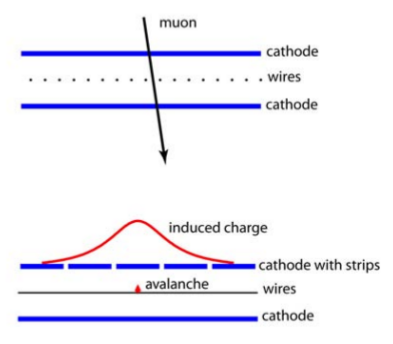
\includegraphics[scale=0.5]{Figures/CSCavalanche.png}
       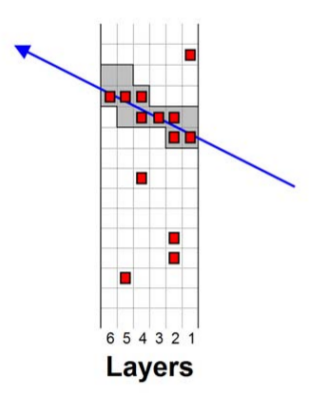
\includegraphics[scale=0.5]{Figures/CSCalct.png} \\
       \caption[A schematic depiction of an avalanche in a cathode strip chamber and an anode local charged track.]{A schematic view of one gap, depicting the principle of CSC operation (right).  The charge induced on the cathode strips is interpolatd, and a localization of the avalanche along the direction of the wire is found.  A pattern of these hits is quickly matched to form an anode local charged track (ALCT, right)~\cite{CMSdetector}.}
\label{figapp:CSCavalanche}
\end{figure}

Each CSC has 5 cathode front end boards (CFEBs) that serve to manage the charge deposited on the cathode strips.  The CFEBs contain more logic than the AFEBs, and use a comparator network that uses on board amplifier shaper outputs to achieve a resolution corresponding to each half strip.  This is achived via a comparison for every group of 3 adjacent strips, determining the amplitude of the central strip signal and comparing it to the central-to-left and central-to-right signal.  Thus if the charge on the central strip is above the threshold, and the charge on the right strip is larger than on the left, the hit position must be in the right half of the central strip.  This is depicted in Figure~\ref{figapp:CSCclct}.

\begin{figure}[!Hh]
       \centering
       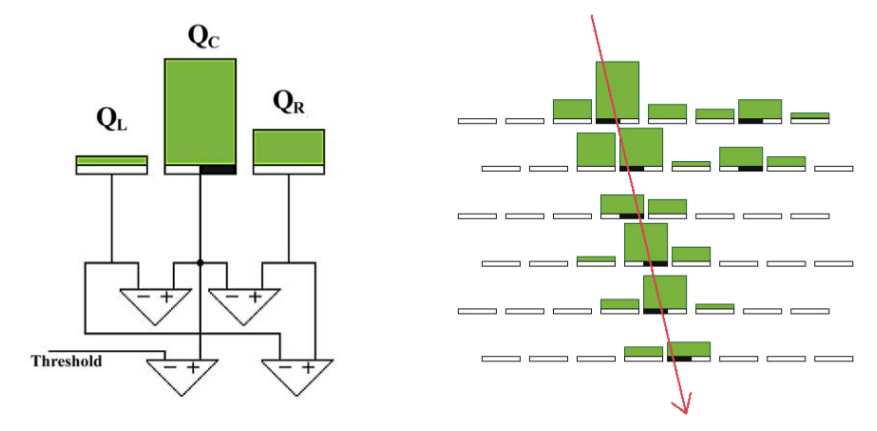
\includegraphics[scale=0.5]{Figures/CSCclct.png} \\
       \caption[A schematic depiction of the formation of a cathode local charged track.]{A schematic depiction of the CFEB comparator network (left) and how half-strip resolution is acheived.  A muon track is depicted in red (right) and the white rectangles represent cathode strips.  Each half-strip where a hit is found is colored black, and the green rectangles represent the amplitude of the signal, showing how the comparator network makes the half-strip decisions~\cite{CMSdetector}.}
\label{figapp:CSCclct}
\end{figure}

The half-strip cathode local charged track hits and the anode local charged track hits are both sent to a piece of off-chamber electronics called the trigger motherboard (TMB).  There is one TMB per chamber, and each can create two 2-dimensional LCTs from the ALCT and CLCT that it receives from the chamber.  These 2D LCTs are sent on to muon port cards (MPCs), each of which collects hits from 9 chambers.  The MPC collects the 2D LCTs, sorts them, and finds the 3 highest quality candidates to send further upstream to the Level-1 muon trigger electronics.  This path is shown in Figure~\ref{figapp:CSCreadout}.

The raw data is collected by the data acquisition, or DAQ, motherboards (DMBs).  They are also located off-chamber, in peripheral crates, with the TMBs and MPC, and there is one per chamber.  The data passed to the DMBs consist of anode and cathode comparator hits in a time window that is up to 32 bunch crossings long.  These data that are collected by the DMB are in turn passed on to the detector dependent unit (DDU) and then to a data concentration card (DCC) and then finally on to the CMS filter farm in order to be processed by the CMS high level trigger (HLT) software.  The approximate event size per chamber is 4-5 kBytes.  These electronics are also shown in Figure~\ref{figapp:CSCreadout}.

If the Level-1 trigger accepts the data from a collision (this decision being made by Level-1 electronics from all subsystems), a ``Level 1 accept'', or L1A, is sent back out.  This signal, as well as the LHC clock and all other control signals, is distributed to all the CSC electronics by the clock control board (CCB).  This is also shown in Figure~\ref{figapp:CSCreadout}.  The raw anode and cathode local charged track data is only sent upstream in coincidence with an L1A signal, so the CSC read-out system is intrinsically zero-suppressed.  

\begin{figure}[!Hh]
%       \centering
       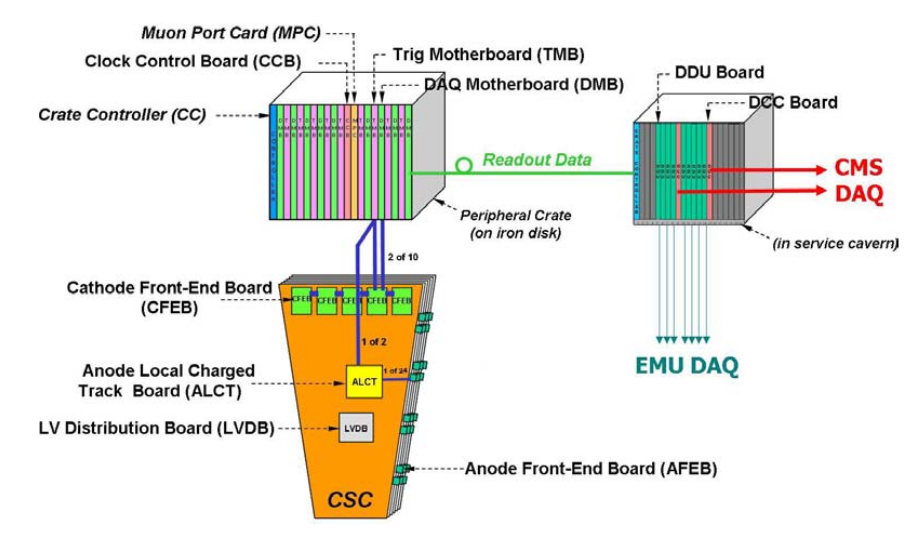
\includegraphics[scale=0.5]{Figures/CSCreadout.png} \\
       \caption[A schematic of the cathode strip chamber electronic trigger and readout system.]{The schematic layout of the cathode strip chamber trigger and read-out electronics~\cite{CMSdetector}.}
\label{figapp:CSCreadout}
\end{figure}


Something about ODMB?



\subsection{The Trigger system}
\label{trigger}


The LHC delivers collisions to the CMS detector at a beam crossing interval of 25ns (or 50ns in 2011 and 2012), corresponding to a crossing frequency of 40 MHz at design parameters.  At this design frequency, and at nominal instantaneous luminosity, an average of 20 collisions per crossing will occur.  As it is impossible to store and process data for some many events, a drastic reduction in the rate of event storage is necessary.  This necessary reduction is performed by the trigger system, which is the the beginning of the physics event selection process.  

The procedure of performing this reduction in rate is separated in to two steps, and thus two systems.  The first is the Level-1 Trigger system (L1 Trigger) and it is composed of custom-designed, mostly programmable electronics.  The second is the High-Level Trigger (HLT), which is a software-based system implemented in a filter farm of approximately one thousand commercial processors.  Combined, the L1 Trigger and HLT effect a rate reduction of at least a factor of $10^6$.  



\subsubsection{The L1 Trigger}
\label{l1trigger}

The design output rate of the L1 Trigger is 100 kHz, which in practice is limited to 30 kHz, with an approximate safety factor of three.  The L1 Trigger uses relatively coarsely segmented data from the calorimeters and the muon system, while keeping the high-resolution data in pipelines in the front-end subdetector electronics.  In order to ensure flexibility, the hardware for the L1 Trigger is implemented in FPGA (Field Programmable Gate Array) technology in most places, but some ASICs and memory lookup tables (LUTs) are also used where speed and radiation resistance is important.  

The L1 Trigger is split in to local, regional, and global components.  At the bottom end, ``closest'' to the subdetectors themselves, the local component called Trigger Primitive Generators (TPGs) are based on energy deposits in the calorimeters and track segments or hit patterns in the muon chambers.  These TPGs are passed to the Regional Triggers which combine their information and use logic to rank and sort trigger objects such as electron or muon candidates in regions limited spatially.  The ranking is determined as a function of energy or momentum and quality, which reflects the confidence in the L1 measurements which is in turn based on the subdetector properties, electronics, and the information available.  The Global Calorimeter and Muon triggers determine the best-quality calorimeter and muon objects across the entire CMS detector and transfer those candidates to the Global Trigger.  The Global Trigger, finally, takes the decision to reject an event or to accept it for further decision making by the HLT.  This decision is based both on algorithmic calculations with the candidate objects and on the readiness of the subdetectors and the data acquisition system (DAQ), and is sent back to the subdetectors via the L1 Accept signal (L1A).  The overall architecture of the L1 Trigger system is shown in Figure~\ref{figapp:L1Tarchitecture}.  

\begin{figure}[!Hh]
%       \centering
       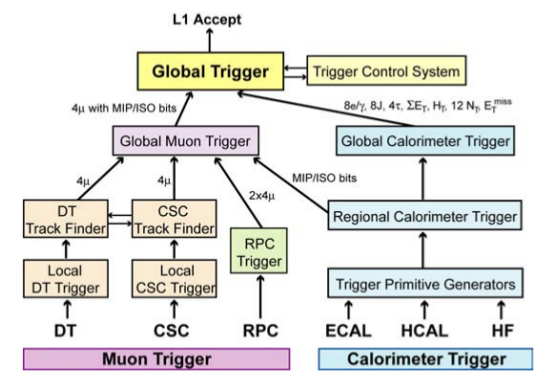
\includegraphics[scale=0.7]{Figures/L1Tarchitecture.png} \\
       \caption[Architecture of the Level-1 Trigger.]{The architecture of the L1 Trigger~\cite{CMSdetector}.  The trigger layers are shown with what information is sent to the Global Trigger: Muons ($\mu$), minimum-ionizing particle and isolation bits (MIP/ISO), electrons and photons ($e/\gamma$), jets (J), taus ($\tau$), total transverse energy ($\Sigma \text{E}_\text{T}$), total hadronic transverse energy($\text{H}_\text{T}$), number of jets passing various transverse energy requirements ($\text{N}_\text{T}$), and missing transverse energy ($\text{E}^\text{miss}_\text{T}$).}
\label{figapp:L1Tarchitecture}
\end{figure}

The TPGs in the Calorimeter Trigger subdivide both calorimeters in to trigger towers.  The TPGs compute the sums of transverse energies measured in the ECAL crystals or HCAL read-out towers in order to obtain the entire trigger tower $\text{E}_T$  and determine the correct bunch crossing.  The TPGs then are transmitted to the Regional Calorimeter Trigger (RCT) which is responsible for multiple tasks.  The RCT determines regional candidates for electrons and photons via determining the tower with the largest energy deposit and then applying two shower profile requirements: a fine-grained crystal energy profile that reflects teh lateral shape of a shower, and a requirement based on the ratio of deposited energies in the hadronic and electromagnetic portions.  It also requires there be at least one quiet corner in one of the course sections surrounding the hit.  This strategy is depicted in Figure~\ref{figapp:CALtrigger}.  The RCT also sums transverse energies in the calorimeters, determines $\tau$-veto bits based on the narrower shape of $\tau$ decays, and produces information relevant for muons in the form of minimum-ionizing particle (MIP) and isolation (ISO) bits.  Finally, the Global Calorimeter Trigger (GCT) determines the jets, total transverse energy and missing transverse energy, jet counts, and the jet-only transverse energy sum given a programmable threshold ($\text{H}_T$).  

\begin{figure}[!Hh]
%       \centering
       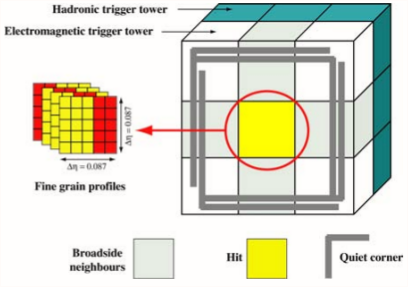
\includegraphics[scale=0.6]{Figures/CALtrigger.png} \\
       \caption[Electron/photon trigger strategy.]{The algorithm the RCT uses for electron/photon triggering~\cite{CMSdetector}.}
\label{figapp:CALtrigger}
\end{figure}

The TPGs in the muon trigger are sourced from all three muons subsystems.  The CSCs in the endcap deliver 3-dimensional track segments (straight line segments, LCTs).  The DTs likewise contribute track segments, which are track segments in the $\phi$-projection and hit pattterns in the $\eta$-projection.  All chambers also identify the bunch crossing from which the event originated from.  The regional muon trigger is based on the DT and CSC Track Finders (DTTF, CSCTF), which serve to create tracks out of the individual segments they receive and thus identify muon candidates along with their transverse momenta, locations, and quality.  The functionality of both the DTTF and CSCTF fits into high-density FPGAs: DTTF segmentation in the central wheel is $2 \times 12$ half-width sectors and in the four outer wheels it is 12 full-width sectors each, while the CSCTF segmentation is by $2 \times 6$ $60^\circ$-sectors.  The CSCTF synchronizes the data and uses extrapolation to form an overall track.  Then the $p_T$ is assigned via lookup tables based on the $\phi$-information from three stations.  The overall strategy for the DTTF is the same, which also uses some pattern matching in the $\eta$ coordinate.  This algorithm is depicted, for the DTTF, in Figure~\ref{figapp:TrackFinder}.  The Global Muon Trigger (GMT) is fed the muon candidates from the DTTF, CSTF, and RPC Trigger and uses them to reduce repeat muon measurements vai merging kinematic parameters and canceling duplicates.  Muons are also back extrapolated to the vertex using the MIP/ISO bits from the calorimeters which are in turn also added to the GMT output.  Finally, the muons are sorted by transverse momentum and quality, to create four candidates to be given to the Global Trigger.

\begin{figure}[!Hh]
       \centering
       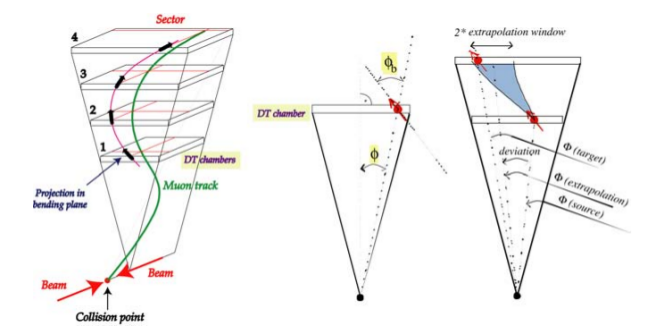
\includegraphics[scale=0.6]{Figures/TrackFinder.png} \\
       \caption[Track Finder track creation scheme.]{The algorithm the DTTF uses for muon candidate track extrapolation~\cite{CMSdetector}.  The CSCTF uses a very similar scheme, with 3-dimensional segments.}
\label{figapp:TrackFinder}
\end{figure}

The Global Trigger (GT) takes the decision to accept or reject an event at Level-1 based on the trigger objects that are delivered to it from the GCT and GMT.  The algorithms vary in complexity, with the most basic ones consisting of applying $p_T$ or $E_T$ thresholds to a single object, or requiring minimum jet multiplicities.  Location and quality information is available as well, so more complex algorithms taking into account event topology cand be programmed.  Up to 128 algorithms can be executed in paralle, and for normal physics data this single trigger mask is applied, with the L1A decision being taken accordingly.  



\subsubsection{The HLT}
\label{hlt}

Unlike the L1 Trigger, the HLT operates on software.  It serves to further reduce the output rate of the L1 Trigger of approximately 30 MHz to 100 Hz.  It consists of a variety of trigger paths based on object kinematics and quality criteria.  However, since it has access to the complete data read-out, it is capable of performing more complex calculations similar to those used by off-line analysis software.  Its goal is to both reduce rate and ensure that events saved match the interest of physics studies, so events are partially reconstructed even in the cases of simple kinematics-based criteria.  HLT algorithms evolve with experience, optimizing the usefullness for off-line analysis.  Additionally, in 2011 and 2012, the instantaneous luminosity delivered by the LHC increased continuosly, so some HLT trigger paths evolved with time to compensate for this and maintain a relatively constant rate of 100 Hz throughout the run periods.  Some HLT triggers also ``prescaled'' events, only saving a sampling of events (saving a $1/N$ fraction of events, where $N$ is called a prescale) that would otherwise increase the rate by large quantities, these prescales were also varied throughout run periods.
 

% Chapter 3
\chapter{Event Reconstruction} % Main chapter title
\label{reco} 

\lhead{Chapter 3. \emph{Event Reconstruction}} % This is for the header on each page - perhaps a shortened title

%----------------------------------------------------------------------------------------

Event reconstruction is the process of computing quantities useful for physics analyses and constructing software objects called ``physics'' objects which are associated quantities that describe the kinematic properties of particles in an event.  It is a software operation which is fundamentally a data reduction procedure whose primary client is the data analysis.  Reconstruction can be divided in to 3 fundamental steps: local reconstruction that occurs within a single subdetector module, global reconstruction that occurs within a whole subdetector system, and the combination of the reconstructed objects to produce higher-level objects.  

Local reconstruction uses as input either real data acquired during runtime that was triggered on by the HLT and stored, or simulated data produced to represent the real data.  The data collected by the DAQ system is in the form of the digitized response of the various subsystems' modules to incident particles (charge avalanches, energy deposits in crystals, etc), so these input data objects are called ``digis'' - a reference to the fact that they are either digitized detector responses or simulations thereof.  The output of local reconstruction software is a reconstruction of the physical hit that occurred in the subdetector module.  Called a ``rechit'', these data objects are typically position measurements taken from times or clusters of strips or pixels in tracking-type subdetector systems (Muon and Tracker), and locations of energy cluster deposits in the calorimeters (ECAL and HCAL).  These rechits are used as input in the following reconstruction step.  

The global reconstruction step occurs separately for each subdetector, in which rechits from multiple subdetector modules are combined.  For instance, rechits from muons are used to produce reconstructed tracks representing candidate muon tracks and rechits in the tracker are used to produce reconstructed charged particle tracks.

Finally, the last step combines the reconstructed data objects from various individual subdetectors to produce the higher-level objects that are ultimately used in high-level triggering and/or for physics analyses.  As an example, a given track in the Tracker subsystem and a track in either the DT or CSC substem (Muon subdetectors) may be combined to form final muon candidates, and likewise electron candidates from the calorimeters are matched to tracks in the Tracker.  

The path that data from a muon takes through this reconstruction algorithm to eventually become a set of kinematics quantities identified as a ``Muon'' is depicted in Figure~\ref{figapp:CMSReco}.  In depth descriptions of the reconstruction of all physics objects follow in sections~\ref{trackreco} through~\ref{pflow}.

\begin{figure}[!Hh]
       \centering
       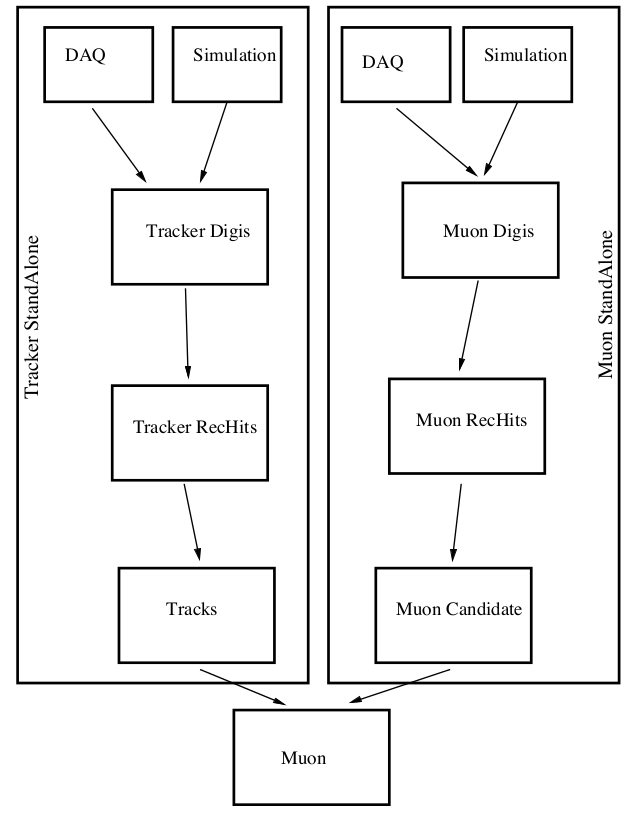
\includegraphics[scale=0.6]{Figures/CMSReco.png} \\
       \caption[A diagram of reconstruction of a muon in CMS.]{An example of a path that data from a muon takes through reconstruction, in the Tracker and Muon subsystems~\cite{CMStdr}.}
\label{figapp:CMSReco}
\end{figure}



\section{Track and Vertex Reconstruction}
\label{trackreco}

Tracks formed by charged particles in the tracking system are reconstructed via an iterative trajectory finding method called the Combinatorial Track Finder (CTF).  This method makes use of both pixel hits and strip hit in in local reconstruction, and pixel hits created via a fast algorithm are used for initial track seeding.  

For ``first-pass'' hit reconstruction, the transverse and longitudinal coordinates are determined via a simple computation.  For each coordinate the cluster is projected on to the respective axis, in the case of a single pixel the center of the pixel is taken, and if there are multiple pixels the hit position is determined using the relative charge of the two pixels at either end.  The position is then corrected for the Lorentz drift of the collected charge in the magnetic field.  These simple hit coordinates are used for track seeding, the first step of the global track reconstruction.  

Over the lifetime of the detector the radiation exposure can significantly impact a pixel module's collection of charge, and thus degrade the performance of the above standard hit reconstruction method.  The hit position can become biased by up to $50 \mu\text{m}$, so a template-based algorthim is used for the steps after track seeding in global track reconstruction~\cite{TrackReco}.  In this method the distribution of charge in the pixel module is compared to expected projected distributions in order to estimate hit positions.  These expected distrubions, called templates, are produced in a simulation called PIXELAV which can include descriptions of behavior of irradiated pixel sensors.  Thus, with updates over the course of the pixel tracker's lifetime, template-based algorithms can maintain a more realistic picture of sensor behavior and thus reduce position bias and improve resolution of the hit reconstruction.  

In the case of hit reconstruction in the strip detector, a seeding method is used.  Clusters are seeded by any channel that is saved offline that has a charge of at least three times the corresponding channel noise.  Neighboring strips are added to this seed if their charge it twice their strip noise, and a cluster overall is kept if the total charge is a factor of five larger than the total cluster noise.  The position of the hit for each cluster is then determined from the charge-weighted average of strip positions, corrected for Lorentz drift as well as for inefficient charge collection near the backplane of the sensitive strip volume.  These strip hits are used in the successive steps of global track reconstruction after seeding.


The global reconstruction of tracks takes the hits in the tracker subdetectors and estimates the momentum and positions of the charged particles responsible for those hits.  The momentum is computed from the bending of the trajectory of the particle in the magnetic field and thus the key role of the global reconstruction is to create these trajectories.  This is performed the software, mentioned above, called the CTF.  The CTF is an adaptation of the combinotorial Kalman filter~\cite{Kalman_Comb1,Kalman_Comb2,Kalman_Comb3} which is a basic Kalman filter~\cite{Kalman_Plain} that includes pattern recognition with track fitting in the same framework.   The CTF process is applied 6 times, iteratively, with the strategy of searching for the tracks that are easiest to find in the first iterations and the tracks that are hardest in the last iterations.  Thus the hits associated with tracks are removed in each iteration, reducing the combinatorial multiplicity in subsequent steps that search for more difficult track classes such as low-$p_T$ or displaced tracks.  Each iteration consists of four steps:

\begin{itemize}
\item{Seed generation begins by providing initial track candidates based on only two or three hits.  The seed contains the initial estimate of trajectory parameters with their uncertainties.}
\item{Finding the track is performed with a Kalman filter, extrapolating the seed trajectories along the expected path and searching for additional hits to be assigned to the track candidate.}
\item{Fitting the track is perfomed with a Kalman filter and smoother, to provide an improved estimate of the parameters of each trajectory.}
\item{Finally, track selection applies a set of quality criteria and discards tracks that fail it, as well as setting various quality flags on passing tracks}
\end{itemize}

The six successive iterations vary in how the inital seed is configured and the criteria applied in the final selection, with the same Kalman filter-based method applied to track finding and fitting.

The resolution of the reconstructed parameters of the tracks is studied using simulated events, using the differences between the generated values and the reconstructed values.  Figure~\ref{figapp:TrackRes} shows the $p_T$ resolution, as a percentage of $p_T$, for singly produced and isolated muons.



\begin{figure}[!Hh]
       \centering
       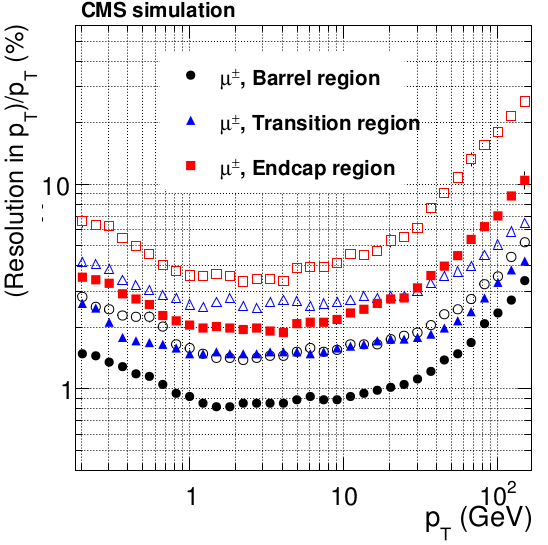
\includegraphics[scale=0.5]{Figures/TrackRes_pt.png} 
       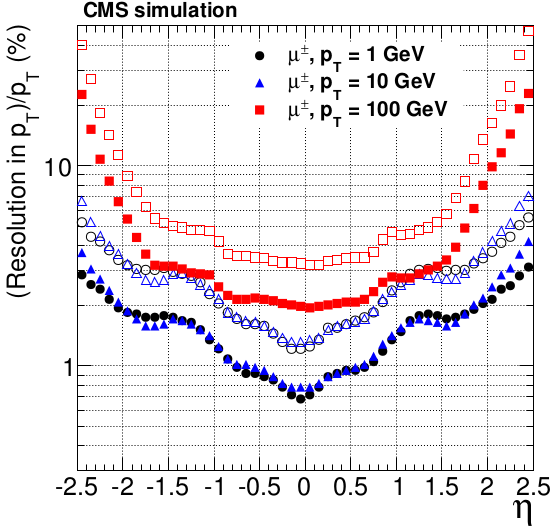
\includegraphics[scale=0.5]{Figures/TrackRes_eta.png} \\
       \caption[Transverse momentum resolution of tracks.]{Resolution of the track $p_T$, for singly produced and isolated muons with $p_T$=1,10, and 100 GeV.  The solid symbols represent the half-width for 68\% intervals, while open represents 90\%~\cite{TrackReco}.}
\label{figapp:TrackRes}
\end{figure}



Reconstruction of the primary vertex aims to measure the location and the associated uncertainty of all the proton-proton interaction vertices in each event, including the ``main'' event and any from pileup collisions, using the reconstructed tracks.  It is perfomed in three steps:


\begin{itemize}
\item{Track selection, in which tracks likely to have been produced ``promptly'' in the primary interaction region are chosen by imposing requirements on the maximum value of significance of the transverse impact parameter relative to the beam spot, the number of strip and pixel hits associated with the track, and the normalized $\chi^2$ from the trajectory fit~\cite{TrackReco}.}
\item{Clustering of tracks that appear to originate from the same interaction vertex, originally performed via simple ordering according to the z-coordinate of the point of closest approach of the tracks to the center of the beamspot and seperated in to different clusters when a given set of coordinates were seperated by more than 2 mm.  Proving a poor choice for high-pileup LHC conditions, this was later changed to a more complex association system called ``deterministic annealing''~\cite{} which included ``soft'' assignments, allowing tracks to be associated with more than one cluster.}
\item{Finally the candidate vertices are fitted to find its position and covariance matrices as well as parameters such as the number of degrees of freedom and weights of tracks used to indicate likelihood of success of the fit.  Each track is assigned a weight between 0 and 1 that reflects the likelihood it belongs to the vertex.}
\end{itemize}

The resolution of the reconstruced primary-vertex position is greatly dependent on the number of tracks used in the fit, as well as the $p_T$ of those tracks.  This dependence is shown in Figure~\ref{figapp:VertexRes}.


\begin{figure}[!Hh]
       \centering
       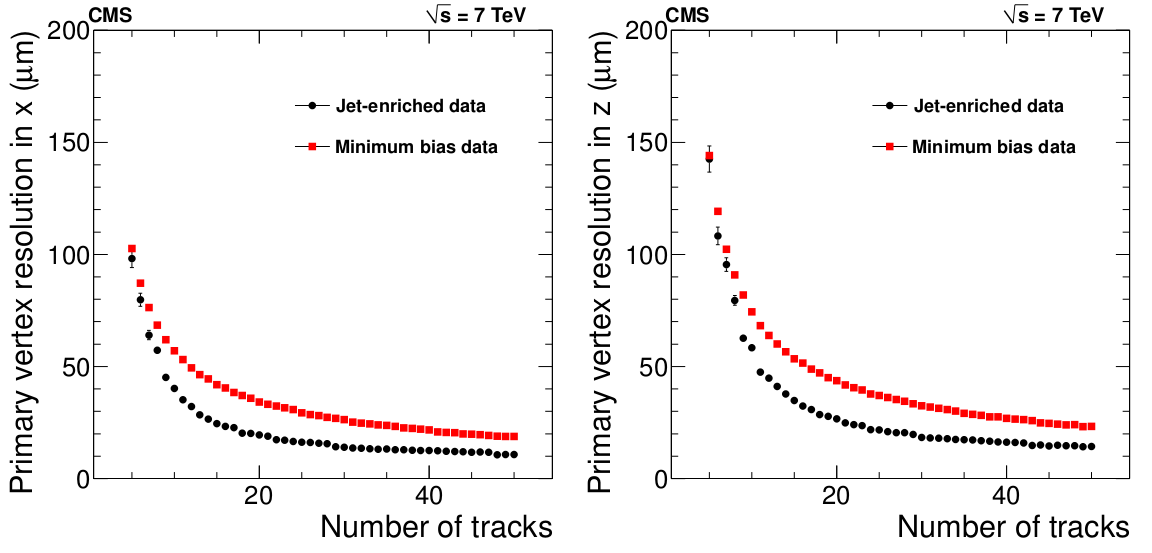
\includegraphics[scale=0.4]{Figures/VertexRes.png} \\
       \caption[Primary vertex resolution as a function of number of tracks.]{Primary vertex resolution as a function of the number of tracks in the vertex.  The jet-enchriched data contains tracks with a significantly higher $p_T$ values~\cite{TrackReco}.}
\label{figapp:VertexRes}
\end{figure}

\section{Muon Reconstruction}
\label{muonreco}

Other than neutrinos and other particles that only weakly interact and cannot be detected in any subdetector in CMS, muons are the only particles that pass through all the detectors inside the magnet solenoid and form tracks in the gas based muon system.  An example of a muon's path through CMS is shown in Figure~\ref{figapp:CMSSlice}.  The CSCs, DTs, and RPCs can form their own muon tracks as well as identify associated tracks from the tracker, and as a result muons are globally reconstructed in both the muon systems and in the tracker system.

\begin{figure}[!Hh]
       \centering
       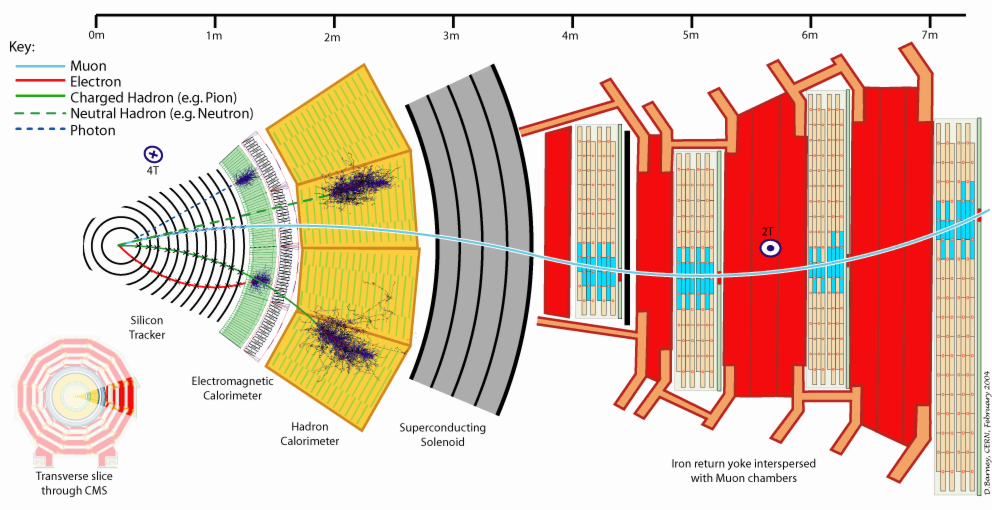
\includegraphics[scale=0.4]{Figures/CMS_Slice.png} \\
       \caption[A transverse slice of the CMS detector]{A slice of a the CMS detector, on the transverse plane, depicting various particles interacting with each specific subsystem.  A muon is shown in blue, traversing the tracker, calorimeters, and magnetic solenoid to leave a track in a muon system.  Its track is bent in two directions, in the inner 4 T field and the outer 2 T field.}
\label{figapp:CMSSlice}
\end{figure}

As with reconstruction in other subsystems, the muon systems begin their reconstruction with local reconstruction - building reconstructed hits either out of simulated data or actual collected data.  The main objects that the DTs use for this are hits in the volume of the drift cells, for which the drift times are converted to drift distances.  Separate $r-/phi$ and $r-z$ projections are combined in to 3-D ``rechits'' and a line segment is formed from aligned hits within the chamber.  The best segment candidate is chosen from any segments sharing hits, and in turn the hit information and segment fit is updated.  

A very similar method is used for the CSCs.  In each of the six layers of a CSC chamber the pulse height is measured to determine the probable hit position, and a 2-D hit is produced with local x and y positions based on the intersection of the locations on the strip and on the wire.  Then a segment is produced by connecting the first and last hits in a chamber, and including any hits within a clustering window along the line connecting those two hits.  This segment must pass a requirement on the resulting $\chi^2$/(number of degrees of freedom) of the fit of those hits that are included.  A minimum of three hits is required for each segment, although segments tend to include closer to the maximum possible 6 hits per segment (due to the 6 layers of the CSCs), as shown in Figure~\ref{figapp:SegmentsPerHit}.

\begin{figure}[!Hh]
       \centering
       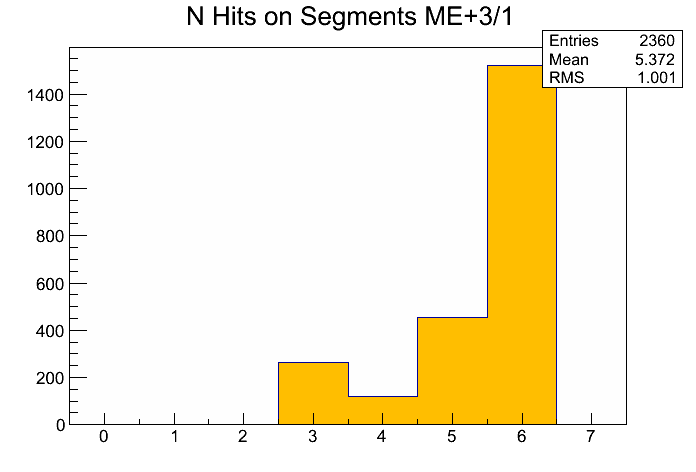
\includegraphics[width=0.45\textwidth]{Figures/Segments_hSnHits+31.png} 
       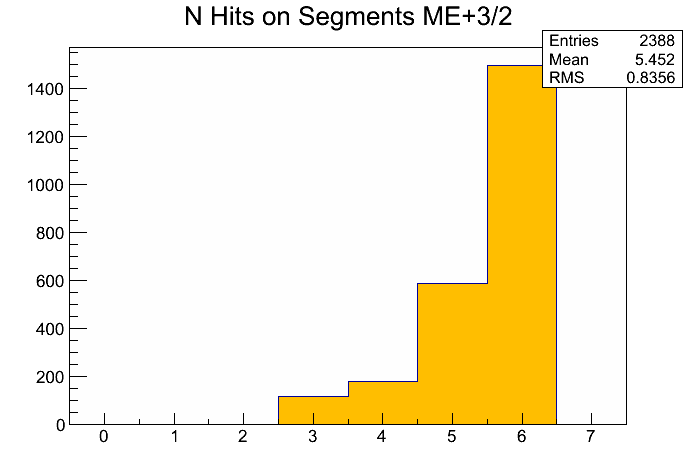
\includegraphics[width=0.45\textwidth]{Figures/Segments_hSnHits+32.png} \\
       \caption[Average hits per segment in a cathode strip chamber]{The average number of hits per segment for a given run in 2012.  The inside disk of the third station of the CSCs (left, ME+3/1) has slightly more ``showered'' muons than the outside disk of the same station (right, ME+3/2).}
\label{figapp:SegmentsPerHit}
\end{figure}

Finally, the RPCs are used in local reconstruction to obtain neighboring clusters with average positions that match the reconstructed hits in either the DTs or the CSCs.

Global reconstruction of muons begins with ``standalone'' reconstruction of tracks only in the muon chambers themselves, also called Level-2 reconstruction.  In standalone reconstruction, the track segments that are built during local reconstruction are used as seeds for muon trajectories.  The track segments from the innermost detectors are taken as state vectors (vectors containing their positions, direction, and momentum, along with covariance matrices) to start an inside-out Kalman fitting procedure~\cite{CMStdr,Kalman_Comb3}.  A predicted state vector is created at the next chamber by using the parameters of the initial state vector and propagating the trajectory outwards.  This projection takes the muon energy loss in the material, the effects of multiple scattering, and the nonuniformity of the magnetic field into account.  At that chamber, assuming that the actual track segment there passes a certain $\chi^2$ requirement, the predicted state is updated with the new information, adjusting parameters of the state vector for the next iteration.  Once the outermost chamber is reached, the ``Kalman Update'' step is complete, and an outside-in fit is performed in the exact same manner, in order to smooth the resulting trajectory.  Together with the ``Kalman Update'', this ``Kalman Smoothing'' step composes the entire Kalman Filter that is applied to the muon track segments.  In the DTs, since each hit is only 2-D, the entire segment is used for this procedure, but the CSC hits are 3-D so each hit is used individually.

Include from http://arxiv.org/pdf/1206.4071.pdf the global reco information, and the muon identification and muon sources information


\begin{figure}[!Hh]
       \centering
       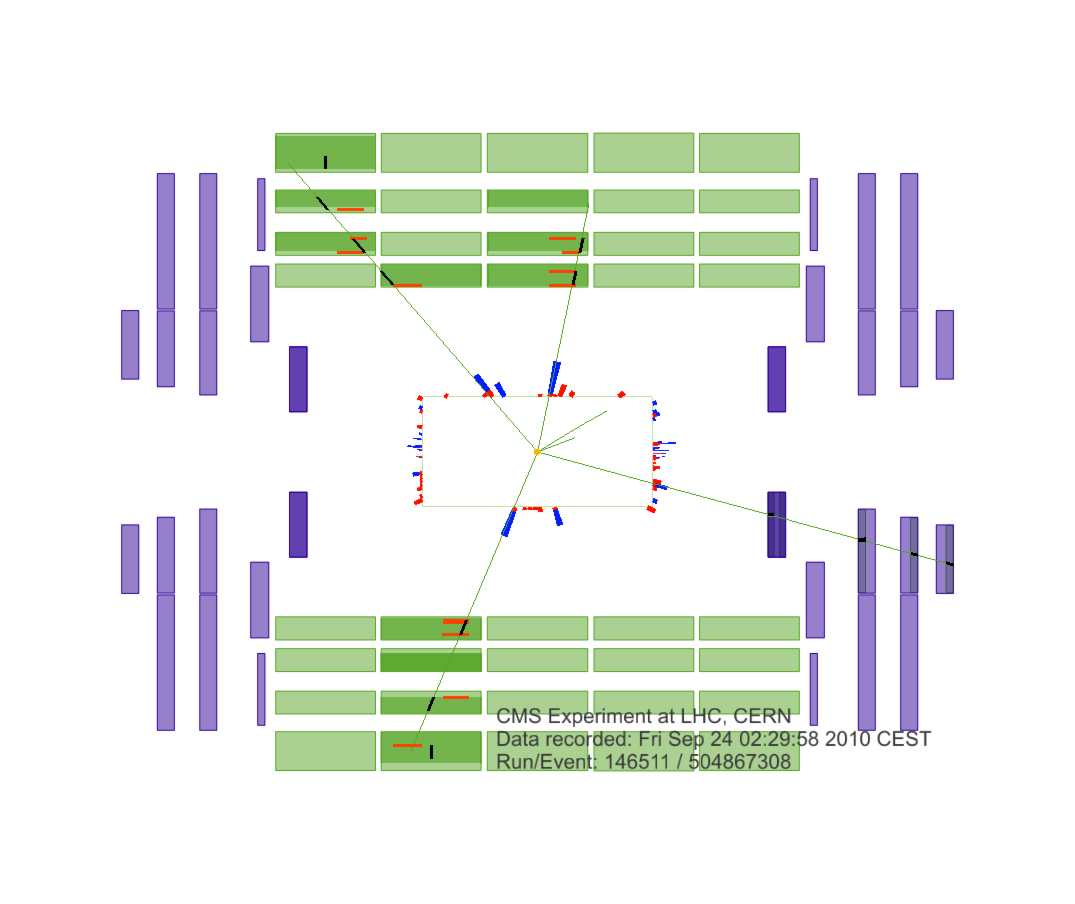
\includegraphics[scale=0.4]{Figures/pictures_r_z_4muon_event_diff_colors_1.png} \\
       \caption[An example of a four muon event in CMS]{A longitudinal view of a collision event in which four muons were reconstructed.  The thin green curves in the inner cylinder represent the tracks of charged particles which were reconstructed in the inner tracker with transverse momentum $p_T > 1\GeV/c$.  Those that extend to the muon system represent the tracks of muons that were reconstructed with both the inner tracker and teh muon system.  Three muons were detected by the DTs and RPCs, and the fourth by the CSCs.  The short black lines in the muon system show segments that were included in the moun track, and the horizontal red lines are depicted the positions of RPC hits.  The energy depositions are shown in red (for ECAL) and blue (for HCAL) on the outer edge of the inner cylinder.~\cite{Chatrchyan:2012xi}}
\label{figapp:ExampleEvent}
\end{figure}


--> muon seeds (from tracker/muon system)
--> L2/standalone reco, just in muon chambers  Kalman filter, propagator with average energy loss, etc, updates
--> L3/global reco with tracker info

--> Something about upgrade for ME0s - improvements of acceptance, etc  go back and put in references that may make sense to build to this point

\section{Electron Reconstruction}
\label{elereco}

\section{Particle flow and jets}
\label{pflow}



\section{Event simulation and detector response}
\label{simulation}

% Chapter 4

\chapter{The Search for Leptoquarks} % Main chapter title

\label{analysis} % For referencing the chapter elsewhere, use \ref{Chapter1} 

\lhead{Chapter 4. \emph{Search for Leptoquarks}} % This is for the header on each page - perhaps a shortened title

%----------------------------------------------------------------------------------------

%\section{placeholder}


Notes:

--> Re iterate signal difficulties, now with plots showing how/what problems it causes
--> Expand each background study section
--> Plot of before and after fiducial cut to show acceptance?  
--> Describe systematics studies in detail
--> Additional kinematics plots
--> Show study of the low pt region?
--> Optimization study - plots/method
--> Include tables in text


\section{Introduction}
\label{introduction}

Leptoquarks (LQ) are hypothetical color-triplet bosons with spin 0 (scalar LQ) or 1 (vector LQ), which are predicted by many extensions of the standard model (SM) of particle physics, such as Grand Unified Theories~\cite{PhysRevLett.32.438,Pati:1973uk,Pati:1974yy,Murayama:1991ah,Fritzsch:1974nn,Senjanovic:1982ex,PhysRevLett.65.2209,Frampton:1990hz}, technicolor schemes~\cite{Dimopoulos:1979es,Dimopoulos:1979sp,Farhi:1980xs}, and composite models~\cite{Schrempp:1984nj}. They carry fractional electric charge ($\pm1/3$ for LQs considered in this paper) and both baryon and lepton numbers and thus couple to a lepton and a quark.  Existing experimental limits on flavor changing neutral currents and other rare processes disfavor leptoquarks that couple to a quark and lepton of more than one SM generation~\cite{Buchmuller:1986iq,FCNC}.  A discussion of the phenomenology of LQs at the LHC can be found elsewhere~\cite{Belyaev:2005ew}.

The production and decay of LQs at proton-proton colliders are characterized by the mass of the LQ particle, $M_{\text{LQ}}$; its decay branching fraction into a charged lepton and a quark, usually denoted as $\beta$; and the Yukawa coupling $\lambda$ at the LQ-lepton-quark vertex. At hadron colliders, leptoquarks could be produced in pairs via gluon fusion and quark anti-quark annihilation, and singly via quark-gluon fusion. Pair production of LQs does not depend on $\lambda$, while single production does, and thus the sensitivity of single LQ searches depends on $\lambda$.  At lower masses, the cross sections for pair production are greater than those for single production.  Single production cross sections decrease more slowly with mass, exceeding pair production at an order of 1 \TeV for $\lambda$ = 0.6.

Several experiments have searched for LQs.  The H1 collaboration has produced limits on various singly produced LQ types: the one to which to compare this search is the LQ called $S^{R}_{0}$ in Ref.~\cite{Collaboration:2011qaa}, for which they place a limit at 500\GeV, assuming $\lambda=1.0$ and $\beta=1.0$.  The \DZERO collaboration has produced limits on singly produced scalar LQs of 274\GeV, again assuming $\lambda=1.0$ and $\beta=1.0$~\cite{Abazov:2006ej}.  Limits from pair production of leptoquarks exclude leptoquark masses below 1010\GeV for the first generation and 1080\GeV for the second generation, for $\beta=1.0$~\cite{PairProd}.

The main single leptoquark production mode at the LHC is the resonant diagram shown in Fig.~\ref{figapp:ResDiagram}.  However, significant contributions are made by the diagrams with non-resonant components shown in Fig.~\ref{figapp:NonResDiagram}.  These contributions increase with both the LQ mass and coupling; the invariant mass distribution of a first generation LQ, of mass $M_{\text{LQ}} = 1$ \TeV and coupling $\lambda=1.0$, possesses a tail extending to very low masses that is comparable to the peak in magnitude.  The reconstructed shape of the resonance peak itself is not strongly affected by $\lambda$.

Also, interference with the $\PQq \Pg \rightarrow \PQq \cPZ/\gamma^{*}\rightarrow \PQq \ell^{+} \ell^{-}$ SM process can occur at dilepton masses in the vicinity of the $\cPZ$ boson mass peak and at lower energies.  Treatments for this interference region and the above-described low-mass off-shell tail of the lepton-jet mass distribution are detailed in Section~\ref{selection}.

The final-state event signatures from the decays of singly produced LQs can be classified as either that of two charged leptons and a jet, where the LQ decays to a charged lepton and a quark, or of a charged lepton, missing transverse energy, and a jet, where the LQ decays into a neutrino and a quark.  The two signatures have branching fractions of $\beta$ and $1-\beta$, respectively.  For this study, and for $S^{R}_{0}$ type LQs, $\beta$ is 1.0, disregarding LQ decays to a neutrino and a quark.  Because the parton distribution functions (PDF) of the proton are dominated by the u and d quarks, the single production of LQs of second and third generation is suppressed.

The charged leptons can be electrons, muons, or taus, corresponding to the three generations of LQs.  In this paper two distinct signatures with charged leptons in the final state are considered: one with two high transverse momentum ($\PT$) electrons and one high-$\PT$ jet (denoted as $\Pe \Pe j$), and the other with two high--$\PT$ muons and one high-$\PT$ jet (denoted as $\Pgm \Pgm j$).

\begin{figure}[!h]
       \centering
       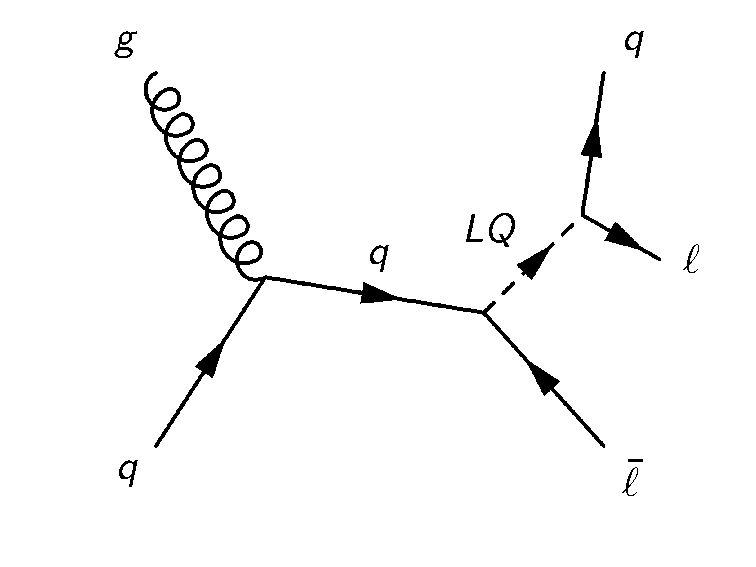
\includegraphics[scale=.45]{Figures/Figures_schannel.pdf} 
       \caption{The $s$-channel resonant LQ production diagram.
	  \label{figapp:ResDiagram}}
\end{figure}

\begin{figure}[!h]
       \centering       
       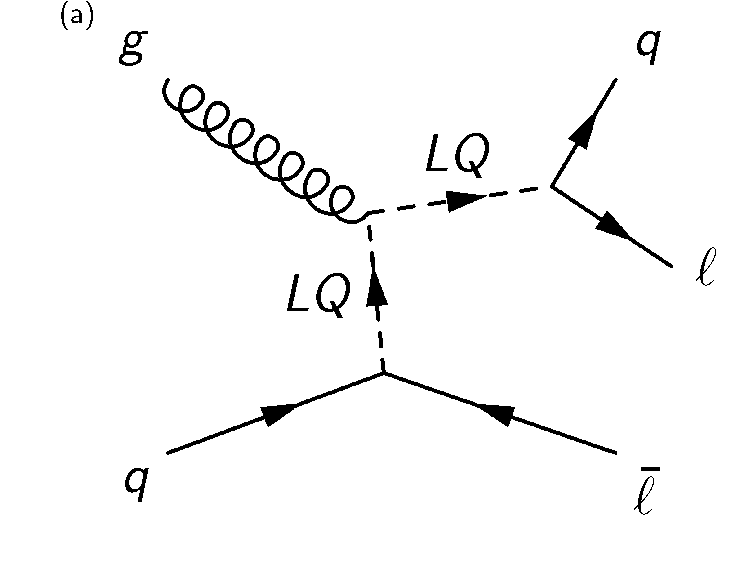
\includegraphics[scale=.45]{Figures/Figures_tchannel1.pdf} 
       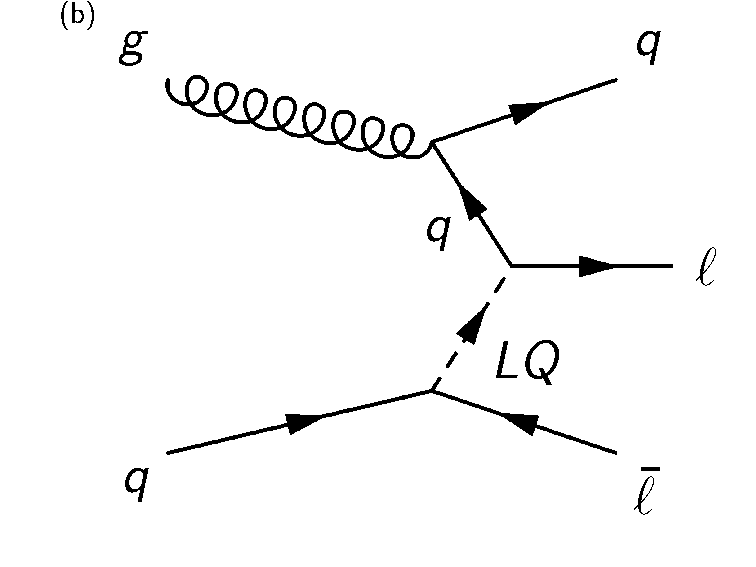
\includegraphics[scale=.45]{Figures/Figures_tchannel2.pdf} 
       \caption{The $t$-channel LQ production diagrams with non-resonant components.  The diagram in (b) is completely non-resonant.
	 \label{figapp:NonResDiagram}}
\end{figure}

\section{The CMS detector}
\label{cms}

The central feature of the CMS apparatus is a superconducting solenoid of 6\unit{m} internal diameter, providing a magnetic field of 3.8\unit{T}.  Within the solenoid volume are a silicon pixel and strip tracker, a lead tungstate crystal electromagnetic calorimeter (ECAL), and a brass and scintillator hadron calorimeter, each composed of a barrel and two endcap sections.  Extensive forward calorimetry complements the coverage provided by the barrel and endcap detectors.  Muons are measured in gas-ionization detectors embedded in the steel flux-return yoke outside the solenoid. 

The ECAL energy resolution for electrons with $\ET \approx 45$\GeV from $\Z \rightarrow \Pe \Pe$ decays is better than 2\% in the central pseudorapidity region of the ECAL barrel $(\abs{\eta} < 0.8)$, and is between 2\% and 5\% elsewhere. For low-bremsstrahlung electrons, where 94\% or more of their energy is contained within a $3 \times 3$ array of crystals, the energy resolution improves to 1.5\% for $\abs{\eta} < 0.8$~\cite{Chatrchyan:2013dga}.

Muons are measured in the pseudorapidity range $\abs{\eta}< 2.4$ with detection planes made using three technologies: drift tubes, cathode strip chambers, and resistive-plate chambers. Matching muon tracks derived from these measurements to tracks measured in the silicon tracker results in a relative \PT resolution for muons with $20 <\pt < 100\GeV$ of 1.3--2.0\% in the barrel and better than 6\% in the endcaps; the \pt resolution in the barrel is better than 10\% for muons with \pt up to 1\TeV~\cite{Chatrchyan:2012xi}.

The first level of the CMS trigger system, composed of custom hardware processors, uses information from the calorimeters and muon detectors to select the most interesting events. The high-level trigger (HLT) processor farm further decreases the event rate from around 100\unit{kHz} to around 400\unit{Hz}, before data storage.

The particle-flow event algorithm reconstructs and identifies each individual particle with an optimized combination of information from the various elements of the CMS detector. The energy of photons is directly obtained from the ECAL measurement, corrected for zero-suppression effects. The energy of electrons is determined from a combination of the electron momentum at the primary interaction vertex as determined by the tracker, the energy of the corresponding ECAL cluster, and the energy sum of all bremsstrahlung photons spatially compatible with originating from the electron track. The energy of muons is obtained from the curvature of the corresponding track. The energy of charged hadrons is determined from a combination of their momentum measured in the tracker and the matching ECAL and HCAL energy deposits, corrected for zero-suppression effects and for the response function of the calorimeters to hadronic showers. Finally, the energy of neutral hadrons is obtained from the corresponding corrected ECAL and HCAL energy.

A more detailed description of the CMS detector, together with a definition of the coordinate system used and the relevant kinematic variables, can be found in~\cite{Chatrchyan:2008zzk}.

\section{Data and simulation samples}
\label{samples}

The data were collected during the 8\TeV pp run in 2012 at the CERN LHC and correspond to an integrated luminosity of 19.6\fbinv.  In the $\Pe \Pe j$ channel, events are selected using a trigger that requires two electrons with $\PT > 33$\GeV and $|\eta| < 2.4$ and in the $\Pgm \Pgm j$ channel, events are selected using a trigger that requires one muon with $\PT > 40$\GeV and $|\eta| < 2.1$.

Simulated samples for the signal processes are generated for a range of leptoquark mass hypotheses between 300 and 3300\GeV and coupling hypotheses between 0.4 and 1.0 in the $\Pe \Pe j$ channel, and a range of leptoquark mass hypotheses between 300 and 1800\GeV and a coupling hypothesis of 1.0 in the $\Pgm \Pgm j$ channel.  Production of LQs in the $\Pgm \Pgm j$ channel is suppressed because of the proton PDF as discussed in Section~\ref{introduction}.

The main sources of background are $\ttbar$, $\cPZ/\gamma^* + {\rm jets}$, $\PW + {\rm jets}$, diboson $(\cPZ\cPZ , \cPZ\PW, \PW\PW) + {\rm jets}$, single top quark, and QCD multijet production.  The $\ttbar + {\rm jets}$ background shape is estimated from a study based on data described in Section~\ref{backgrounds}; the simulation sample for the normalization of the $\ttbar + {\rm jets}$ background as well as the samples for the $\cPZ/\gamma^* + {\rm jets}$ and $\PW + {\rm jets}$ backgrounds are generated with \MADGRAPH 5.1~\cite{MadGraph}.  Single top quark samples ($\PQs$-, $\PQt$-channels, and $\PW$ boson associated production) are generated with \POWHEG 1.0~\cite{POWHEG,Alioli:2009je,Frixione:2007vw,Nason:2004rx} and diboson samples are generated with \PYTHIA (version 6.422)~\cite{PYTHIA} using the Z2 tune~\cite{tunez2}.  The QCD multijet background is estimated from data.  

For the simulation of signal samples, the {{\textsc{CalcHEP}}\xspace}~\cite{hepmdb} generator is used for calculation of the matrix elements. The signal cross sections are computed at leading order (LO) with {{\textsc{CalcHEP}}\xspace} and are listed in Table~\ref{tab:sigxsectionscombined} in the appendix.  Blank entries were not considered because of the small size of the cross section. The resonant cross sections $\sigma_{\text{res}}$ are shown in Fig.~\ref{figapp:CrossSections} and are defined by the kinematics selections given in Section~\ref{selection}.

The \PYTHIA and \MADGRAPH simulations use the CTEQ6L1~\cite{CTEQ} PDF sets, those produced with {{\textsc{CalcHEP}}\xspace} use the CTEQ6L PDFs, and the \POWHEG simulation uses the CTEQ6m set.  All of the simulations use \PYTHIA for the treatment of parton showering, hadronization, and underlying event effects.  For both signal and background simulated samples, the simulation of the CMS detector is based on the \GEANTfour package~\cite{GEANT4}.  All simulated samples include the effects of extra collisions in a single bunch crossing as well as collisions from nearby bunch crossings (out-of-time pileup and in-time pileup, respectively).  The pileup profiles in simulation are reweighted to the distributions of the reconstructed vertices per bunch crossing in data collected by the CMS detector.

\begin{figure}[!h]
       \centering
       {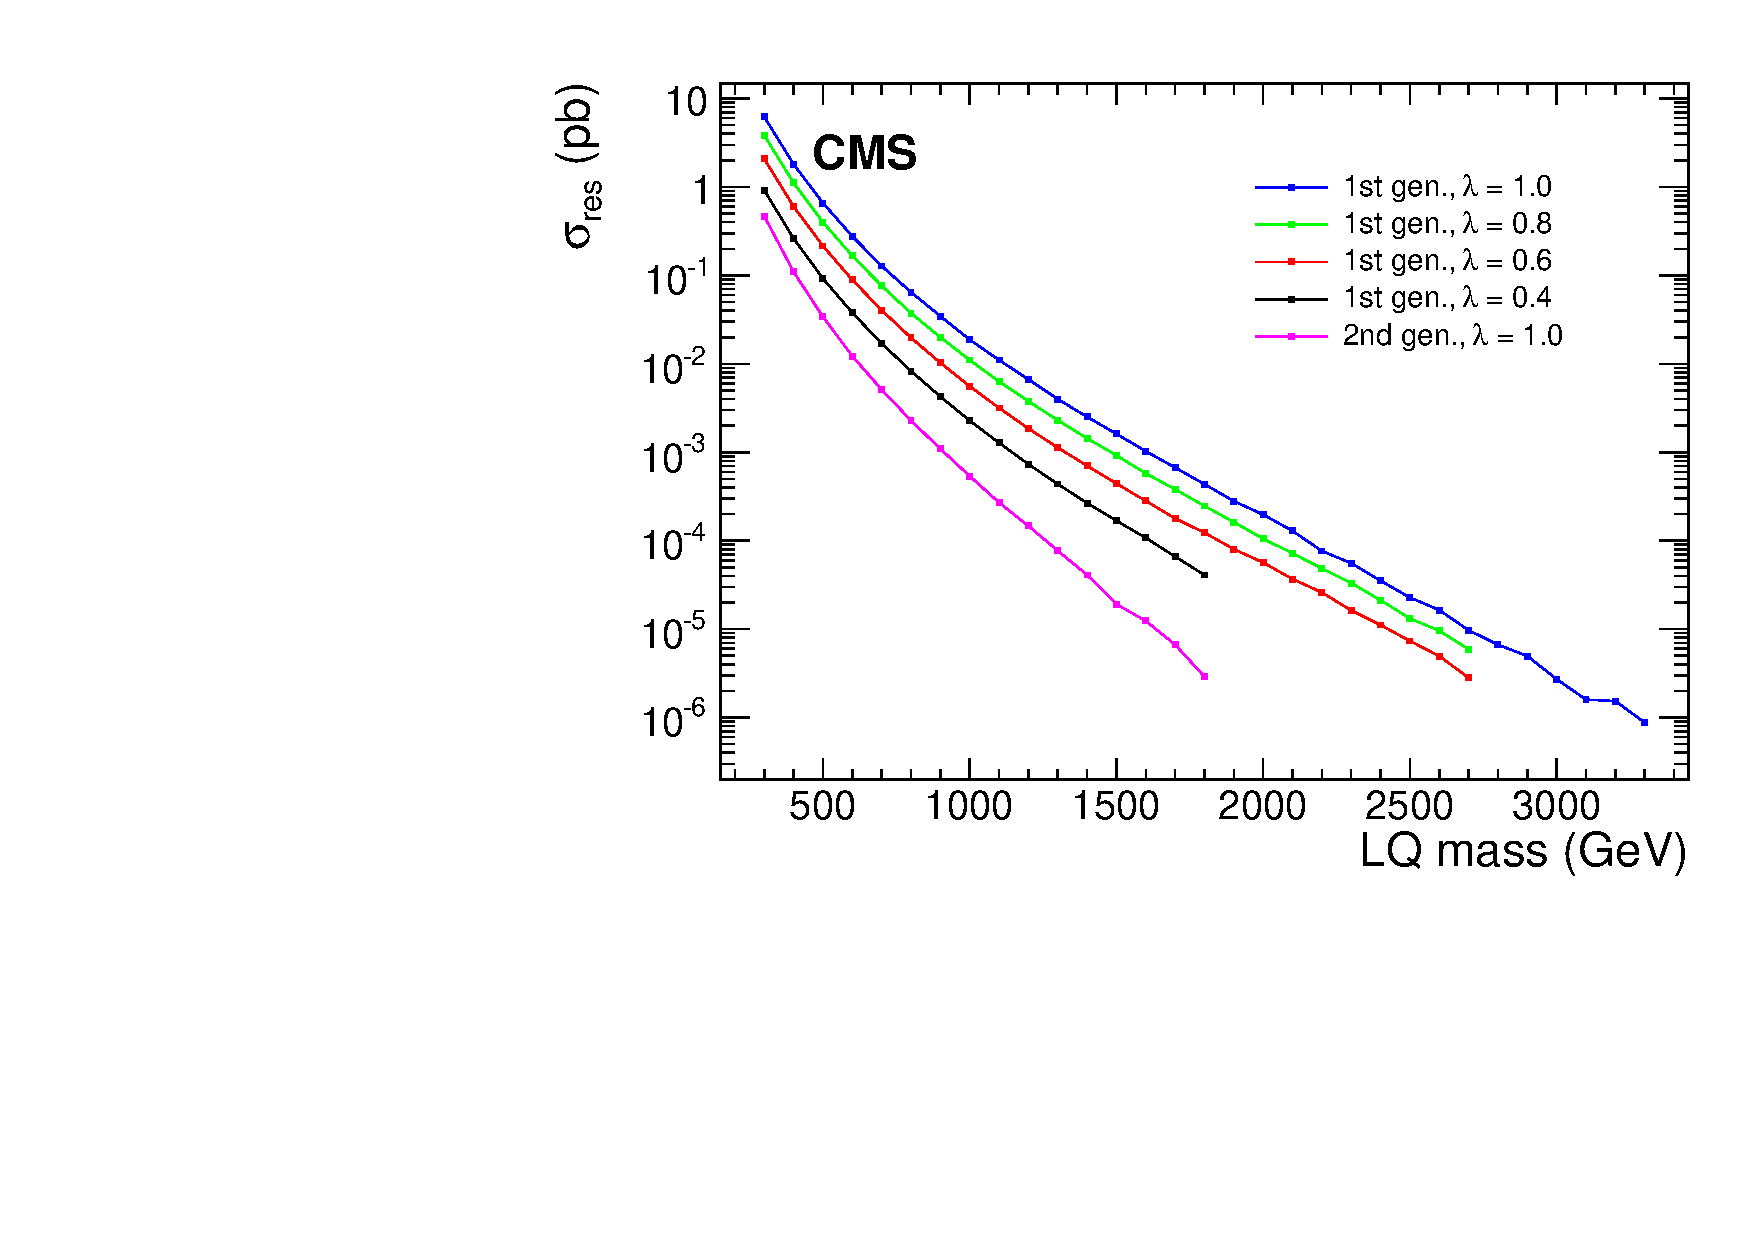
\includegraphics[width=.45\textwidth]{Figures/Figures_CrossSections.pdf}}
       \caption{Cross sections for single LQ production, calculated at LO in {{\textsc{CalcHEP}}\xspace} and scaled by the acceptance of the requirements described in Section~\ref{selection}, as a function of the LQ mass in \GeVns.
	 \label{figapp:CrossSections}}
\end{figure}

In the $\Pe \Pe j$ channel, the background and signal are rescaled by a uniform trigger efficiency scale factor of 0.996, which is measured in~\cite{CMS-PAPERS-EXO-12-061}.
In the $\Pgm \Pgm j$ channel, the background and signal are rescaled by muon $\eta$-dependent efficiency factors of 0.94 $(|\eta| \le 0.9$), 0.84 ($0.9 < |\eta| \le 1.2$), and 0.82 ($1.2 < |\eta| \le 2.1$).  An uncertainty of 1\% is assigned to these factors to account for variations during data-taking periods and statistical uncertainties.  

\section{Event reconstruction}
\label{objectreco}

Muons are reconstructed as tracks in the muon system that are ``globally'' matched to reconstructed tracks in the tracking system~\cite{Chatrchyan:2012xi}.  Muons are required to have $\PT > 45$\GeV and $|\eta| < 2.1$.  Additionally, they are required to satisfy a set of criteria that is optimized for high $\PT$; they are reconstructed as ``global'' muons with tracks associated to hits from at least two muon detector planes together with at least one muon chamber hit that is included in the "global" track fit~\cite{Chatrchyan:2012xi}.  To perform a precise measurement of the \PT and to reduce background from muons from secondary decays in flight, at least eight hits are required in the tracker and at least one in the pixel detector.   To minimize background from muons from cosmic ray backgrounds, the transverse impact parameter with respect to the primary vertex is required to be less than 2 mm and the longitudinal distance is less than 5 mm.  Muons are required to be isolated by applying an upper threshold on the relative tracker isolation of 0.1.  The relative tracker isolation is defined as the ratio of the \PT of all tracks in the tracker coming from the same vertex, excluding the muon candidate track, in a cone of {$\Delta R = \sqrt{\smash[b]{(\Delta \phi) ^2 + (\Delta \eta) ^2}} = 0.3$} (where $\phi$ is the azimuthal angle in radians) around the muon candidate track, and the muon \PT.

Electrons are required to have a reconstructed track in the central tracking system that is matched in $\eta$ and $\phi$ to a cluster of ECAL crystals that has a shape consistent with an electromagnetic shower.  The transverse impact parameter of the track with respect to the primary vertex is required to be less than 2 mm for electrons in the barrel ($\abs{\eta} < 1.442$) and less than 5 mm for electrons in the endcap ($\abs{\eta} > 1.560$).  Electrons are required to be isolated from reconstructed tracks other than the matched track in the central tracking system and from additional energy deposits in the calorimeter.  To reject electrons coming from photon conversions within the tracker material, the reconstructed electron track is required to have hits in all pixel layers.  Electrons in the analysis have $\PT > 45$\GeV and $|\eta| < 2.1$ to match the muon requirements (excluding the transition region between barrel and endcap detectors, $1.442  < \abs{\eta} < 1.560 $).  Selection criteria for electron identification and isolation optimized for high energies are also applied~\cite{CMS-PAPERS-EXO-12-061}.

Jets are reconstructed with the CMS particle-flow algorithm~\cite{CMS-PAS-PFT-09-001,CMS-PAS-PFT-10-001}, which measures
stable particles by combining information from all CMS subdetectors. The jet reconstruction algorithm used
in this paper is the anti-k$\rm _T$~\cite{Cacciari:2008gp,fastjetmanual} algorithm with a
distance parameter $0.5$, which only considers tracks associated to the primary vertex. Jet momentum is determined as the vectorial sum of all particle momenta in the jet, and is found from simulation to be within 5\% to 10\% of the true momentum over the whole \pt spectrum and detector acceptance.  An offset correction is applied to jet energies to take into account the contribution from additional proton-proton interactions within the same bunch crossing. Jet energy corrections are derived from simulation, and are confirmed with in situ measurements of the energy balance in dijet and photon+jet events~\cite{CMS-PAPERS-JME-10-011}. Additional selection criteria are applied to each event to remove spurious jet-like features originating from isolated noise patterns in certain HCAL regions.  The jet energy resolution amounts typically to 15\% at 10\GeV, 8\% at 100\GeV, and 4\% at 1\TeV, to be compared to about 40\%, 12\%, and 5\% obtained when the calorimeters alone are used for jet clustering.

Jets are required to have $\PT>45$\GeV, $|\eta| < 2.4$, and an angular separation from leptons of $\Delta R > 0.3$.

\section{Event selection}
\label{selection}

We require that events in both the $\Pe \Pe j$ and $\Pgm \Pgm j$ channels contain at least two leptons and at least one jet that satisfy the above identification criteria.  Additional kinematic requirements are applied to remove regions in which the trigger and identification criteria are not at plateau efficiency and to reduce large backgrounds.  This creates a basic preselection region:  the jet $\PT$ must be larger than 125\GeV, the dilepton invariant mass $M_{\ell\ell} $ must be larger than 110\GeV, and the scalar sum of transverse momenta of objects in the event ($\ST = \PT(\ell_1)+\PT(\ell_2)+\PT(j_1)$) is required to exceed 250\GeV, where $\ell_1$ is the highest $\PT$ lepton in the event, $\ell_2$ is the second-highest $\PT$ lepton, and $j_1$ is the highest $\PT$ jet.  The two leptons in the events are required to have opposite charges.  

After this initial selection, a final selection is optimized for each channel separately by maximizing $S/\sqrt{S+B}$, where $S$ is the number of signal events in the simulation passing a given selection and $B$ is the number of background events in the simulation passing the same selection.  We optimize for each LQ mass hypothesis by varying the requirements on $M_{\ell j}$ and $\ST$.

As discussed in Section~\ref{introduction}, owing to the unique aspects of single LQ decays, two generator level requirements are applied to the simulated signal samples.  The first is $M_{\ell\ell} > 110$\GeV, to remove LQ decays that are in the Z boson interference region.  The second is a requirement on $M_{\ell j}$, defined as the higher of the two possible lepton-jet mass combinations, chosen to remove the $t$-channel diagram contributions in the low-mass off-shell region, while preserving most of the resonant signal.  This requirement is set at $M_{\ell j} > 0.67 \, M_{\text{LQ}}$ for the first-generation studies and $M_{\ell j} > 0.75 \, M_{\text{LQ}}$ for the second-generation studies.  The thresholds for $M_{\ell j}$ were chosen separately for each channel, because of the differences in the distribution shape.  The dilepton invariant mass requirement at the generator level precisely matches the reconstruction level requirement at the preselection.  These two requirements define the resonant region.  Cross sections at the generator level before and after these requirements are provided in Table~\ref{tab:sigxsectionscombined}, in the appendix.

The $\Pe \Pe j$ channel selection after optimization is identical for all couplings.  The threshold on $\ST$ starts at 250\GeV for $M_{\text{LQ}}=300$\GeV and increases linearly until it reaches a plateau value of 900\GeV at $M_{\text{LQ}}=1125$\GeV.  The $M_{\ell j}$ threshold starts at 200\GeV for $M_{\text{LQ}}=300$\GeV and increases linearly until it plateaus at 1900\GeV above $M_{\text{LQ}}=2000$\GeV.  In the $\Pgm \Pgm j$ channel after optimization the threshold on $\ST$ starts at 300\GeV for $M_{\text{LQ}}=300$\GeV and increases linearly until it plateaus at 1000\GeV above $M_{\text{LQ}}=1000$\GeV.  The $M_{\ell j}$ threshold starts at 200\GeV for $M_{\text{LQ}}=300$\GeV and increases linearly until it plateaus at 800\GeV above $M_{\text{LQ}}=900$\GeV.  The exact threshold values are listed in Tables \ref{tab:optimizedcuts1p0} and \ref{tab:optimizedcutscmu} in the appendix.

\section{Background estimations}
\label{backgrounds}

The SM processes that mimic the signal signature are $\cPZ/\gamma^* + {\rm jets}$, $\ttbar$, single top quark, diboson $ + {\rm jets}$, $\PW + {\rm jets}$, and QCD multijets events where the jets are misidentified as leptons.  The dominant contributions come from the former two processes, whereas the other processes provide minor contributions to the total number of background events. 
 
The contribution from the $\cPZ/\gamma^* + {\rm jets}$ background is estimated with a simulated sample that is normalized to agree with data at preselection in the $\cPZ$-enriched region of $80 < M_{\ell\ell} < 100$\GeV, where $M_{\ell\ell}$ is the dilepton invariant mass.  With this selection the data sample (with non-$\cPZ/\gamma^* + {\rm jets}$ simulated samples subtracted) is compared to $\cPZ/\gamma^* + {\rm jets}$ in simulation.  The resulting scale factor, representing the ratio of the measured yield to the predicted yield, is $R_{\cPZ} = 0.98 \pm 0.01 \stat$ in both the $\Pe \Pe j$ and $\Pgm \Pgm j$ channels.  This scale factor is then applied to the simulated $\cPZ/\gamma^* + {\rm jets}$ sample in the signal region of $M_{\ell\ell} > 110$\GeV.  In order to account for possible mismodeling of the $\PT(\ell\ell)$ spectrum of the $\cPZ/\gamma^* + {\rm jets}$ background sample, where $\PT(\ell\ell)$ is the scalar sum of the two highest \PT leptons in the event, we perform a bin-by-bin rescaling of yields at preselection and full selection by scale factors measured in an inverted $M_{\ell\ell}$ selection ($M_{\ell\ell} < 110$\GeV).  These scale factors differ from unity by 1\% to 10\%, depending on the $\PT(\ell\ell)$ bin, and are applied to the $\cPZ/\gamma^* + {\rm jets}$ sample in the signal region of $M_{\ell\ell} > 110$\GeV.

We estimate the $\ttbar$ background with a $\ttbar$-enriched $\Pe \Pgm$ sample in data, selected using the single muon trigger.  We use a selection that is identical to our signal selection in terms of kinematics requirements, except that we require at least a single muon and a single electron rather than requiring two same-flavor leptons.   The $\Pe \Pgm$ sample is considered to be signal-free, because limits on flavor changing neutral currents imply that LQ processes do not present a different-flavor decay topology~\cite{Buchmuller:1986iq,FCNC}. The $\ttbar$ background is largely dominant in the $\Pe \Pgm$ sample with respect to the other backgrounds.  The sample is normalized to account for the different branching fractions of the $\Pe \Pgm$ and $\Pe \Pe$ or $\Pgm \Pgm$ final states ($B(\Pe \Pgm) = 2\, B(\Pe \Pe\text{ or }\Pgm \Pgm)$) and the difference in electron and muon identification and isolation efficiencies, collectively taken to be $R_{(\Pe \Pe \text{ or } \Pgm \Pgm)/\Pe \Pgm}$, for the two channels.  The sample is also normalized by the ratio of the single-muon trigger efficiency and either the double-electron trigger efficiency or single-muon trigger efficiency in two muon final states ($R_{\text{trig},(\Pe \Pe \text{ or } \Pgm \Pgm)}$).  The overall normalization is taken from simulation and the $\Pe \Pgm$ sample is taken from data.  The $\Pe \Pgm$ sample is then used to estimate the contribution from $\ttbar$ at preselection and final selection.  The number of estimated $\ttbar$ events, $N^{\ttbar, \text{est}}$, is 

\begin{eqnarray}
N^{\ttbar, \text{est}} &=& (N^{\Pe \Pgm, \text{data}}-N^{\Pe \Pgm, \text{non-}\ttbar \text{ sim}}) \times \nonumber \\
 & & \ \, R_{(\Pe \Pe \text{ or } \Pgm \Pgm)/\Pe \Pgm} \, R_{\text{trig}, (\Pe \Pe \text{ or } \Pgm \Pgm)}
,
\label{eq:ttbar}
\end{eqnarray}

with
\begin{equation}
R_{\text{trig},\Pe \Pe} = \frac{\epsilon_{\Pe \Pe}}{\epsilon_{\Pgm}}
,
\label{eq:ttbarratio}
\end{equation}

\begin{equation}
R_{\text{trig},\Pgm \Pgm } = \frac{1-(1-\epsilon_{\Pgm})^{2}}{\epsilon_{\Pgm}} = 2-\epsilon_{\Pgm}
,
\label{eq:ttbarratiomumu}
\end{equation}

where $\epsilon_{\Pgm}$ and $\epsilon_{\Pe \Pe}$ are the single-muon trigger and double-electron trigger efficiencies, respectively, and $N^{\Pe \Pgm, \text{data}}$ and $N^{\Pe \Pgm, \text{non-}\ttbar \text{ sim}}$ are the number of events observed in data and in other backgrounds in the $\Pe \Pgm$ sample, respectively.  $R_{\text{trig},\Pgm \Pgm }$ is the ratio of the efficiency of a single muon trigger on a dimuon sample over the efficiency on a single muon sample (the numerator is the likelihood of failure on two muons).

The contribution from QCD multijet processes is determined by a method that makes use of the fact that neither signal events nor events from other backgrounds produce final states with same-charge leptons at a significant level.  We create four selections, with both opposite-sign (OS) and same-sign (SS) charge requirements, as well as isolated and non-isolated requirements.  Electrons in isolated events must pass the isolation criteria optimized for high-energy electrons~\cite{CMS-PAPERS-EXO-12-061} and muons are required to have a relative tracker isolation less than 0.1, as discussed in Section~\ref{objectreco}.  Non-isolated events are those with leptons failing these criteria.  The four selections are as follows,

\begin{equation}
\sloppy
\left( \begin{array}{cc}
  A & B  \\
  C & D  
\end{array} \right) = 
\left( \begin{array}{cc}
  \text{OS+isolated} & \text{OS+non-isolated}  \\
  \text{SS+isolated} & \text{SS+non-isolated}  
\end{array} \right).
\label{eq:ACBDMatrix}
\end{equation}

The shape of the background is taken from the SS region with isolation requirements, and the normalization is obtained from the ratio between the number of OS events and the number of SS events in the non-isolated selection.  Thus, the number of events, $N^{\text{QCD, est}}$, is estimated by 

\begin{equation}
\small{
N^{\text{QCD, est}} = r_{B/D} \, N_{C}^{(\text{data -- non-QCD sim})}
},
\label{eq:QCD_ABCDeq}
\end{equation}

where $N_{C}^{(\text{data -- non-QCD sim})}$ is the number of events in region $C$ of Eq. (\ref{eq:ACBDMatrix}) and $r_{B/D}$ is the ratio of the number of events (measured in data with simulated non-QCD backgrounds subtracted) in regions $B$ and $D$.  The result is that QCD multijet processes account for 2\% (1\%) of the total SM background in the $\Pe \Pe j$ ($\Pgm \Pgm j$) channel.

The contributions of the remaining backgrounds (diboson+jets, \PW+jets, single top quark) are small and are determined entirely from simulation.

The preselection level distributions in $M_{\Pe \Pe}$, $\ST$, and $M_{\ell j}$ are shown in Figs.~\ref{figapp:elemisc} and~\ref{figapp:muonmisc} for the observed data and estimated backgrounds, where they are compared with a signal LQ mass of 1000\GeV in the $\Pe \Pe j$ channel, and with a signal LQ of mass 600\GeV, in the $\Pgm \Pgm j$ channel.  In all plots the $\cPZ/\gamma^* + {\rm jets}$ prediction is normalized to data and the $\ttbar$ prediction is taken from the study based on data.  Data and background are found to be in agreement.  The numbers of events selected in data and in the backgrounds at each final selection (for each hypothesis mass) are shown in Tables~\ref{tab:eenumbers1p0},~\ref{tab:eesignumbers1p0}, and~\ref{tab:mumunumbers} in the appendix.

The observed data and background predictions are compared after final selection for $\lambda = 0.4$ and a signal LQ mass of 1000\GeV in the $\Pe \Pe j$ channel and a signal LQ mass of 600\GeV in the $\Pgm \Pgm j$ channel and are shown in Figs.~\ref{figapp:elefinalsel} and~\ref{figapp:mufinalsel}.

\begin{figure}[!htb]
       \centering
       {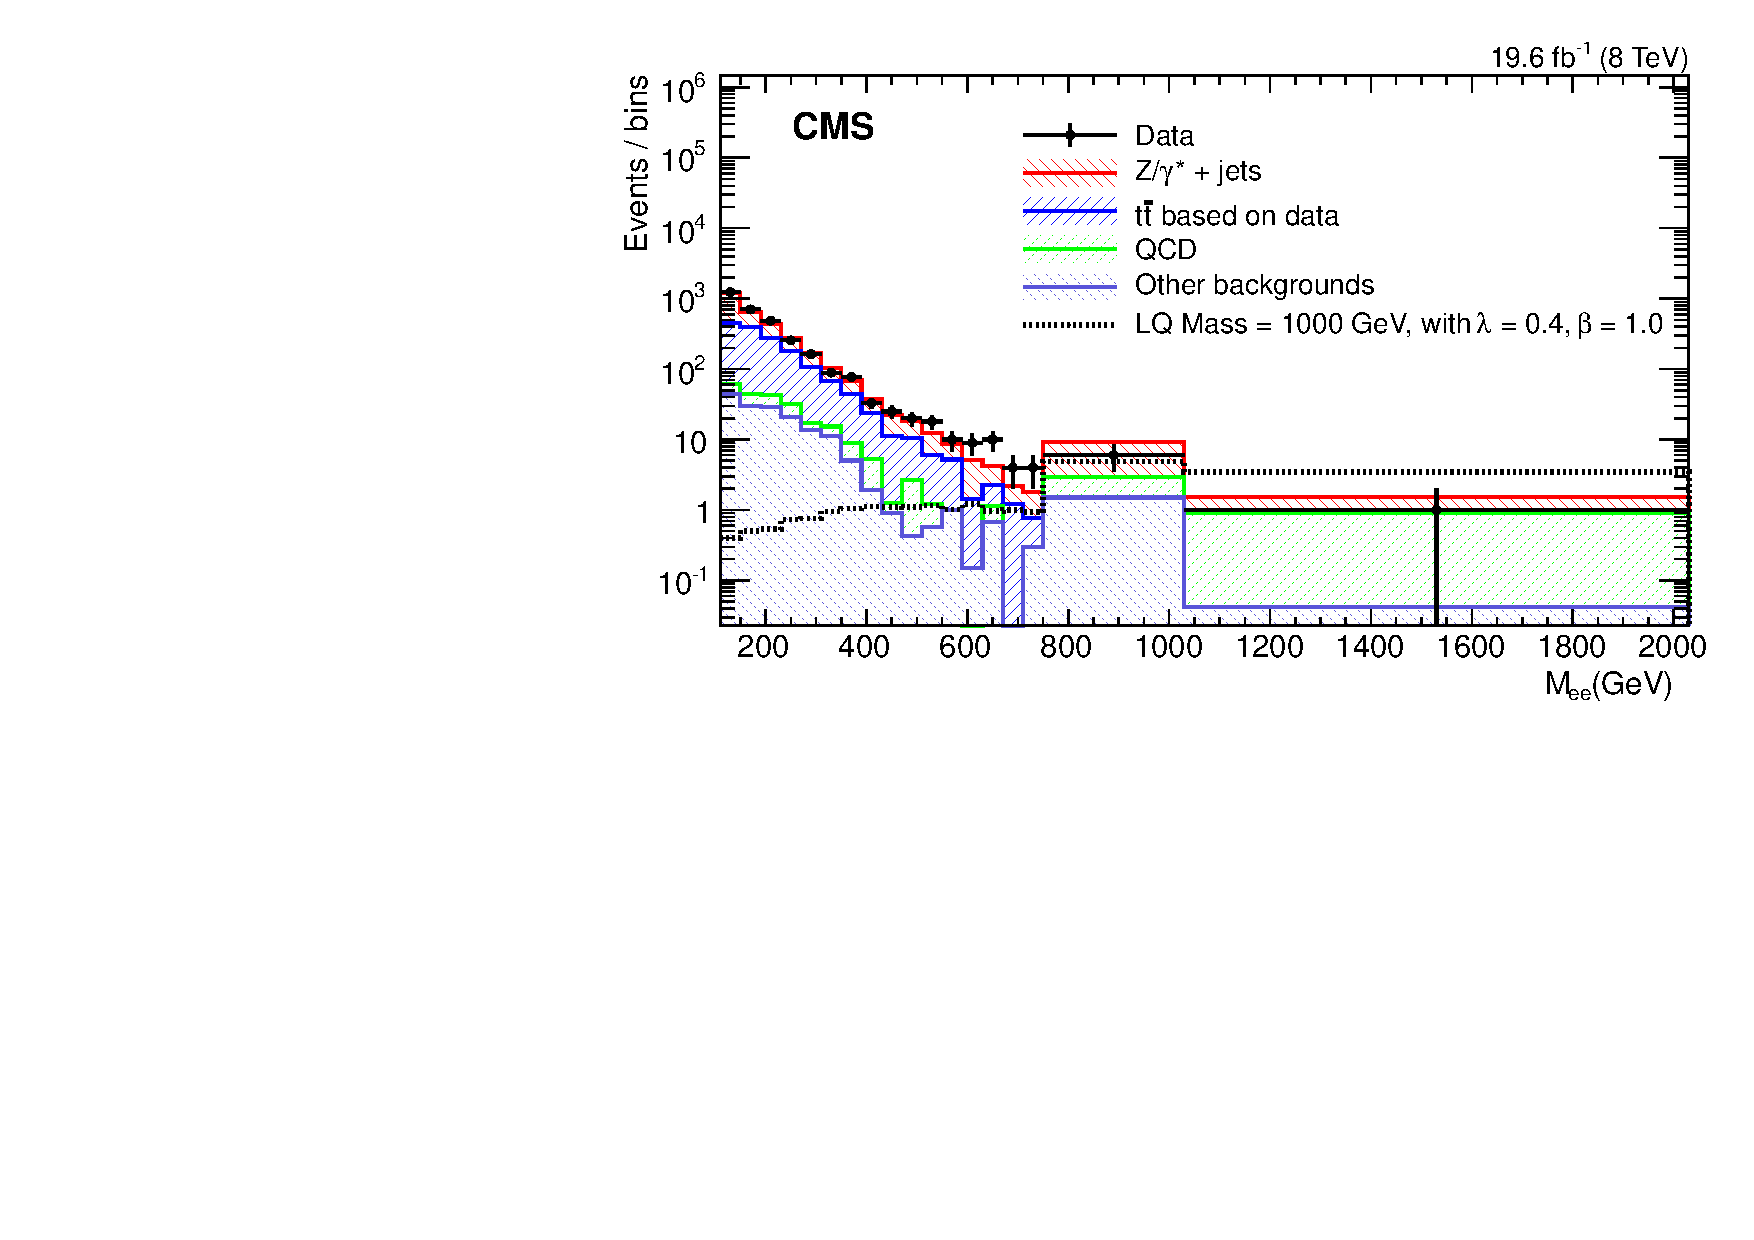
\includegraphics[width=.75\textwidth]{Figures/Figures_ee_M_HEEPele1ele2_Preselection.pdf}}
       {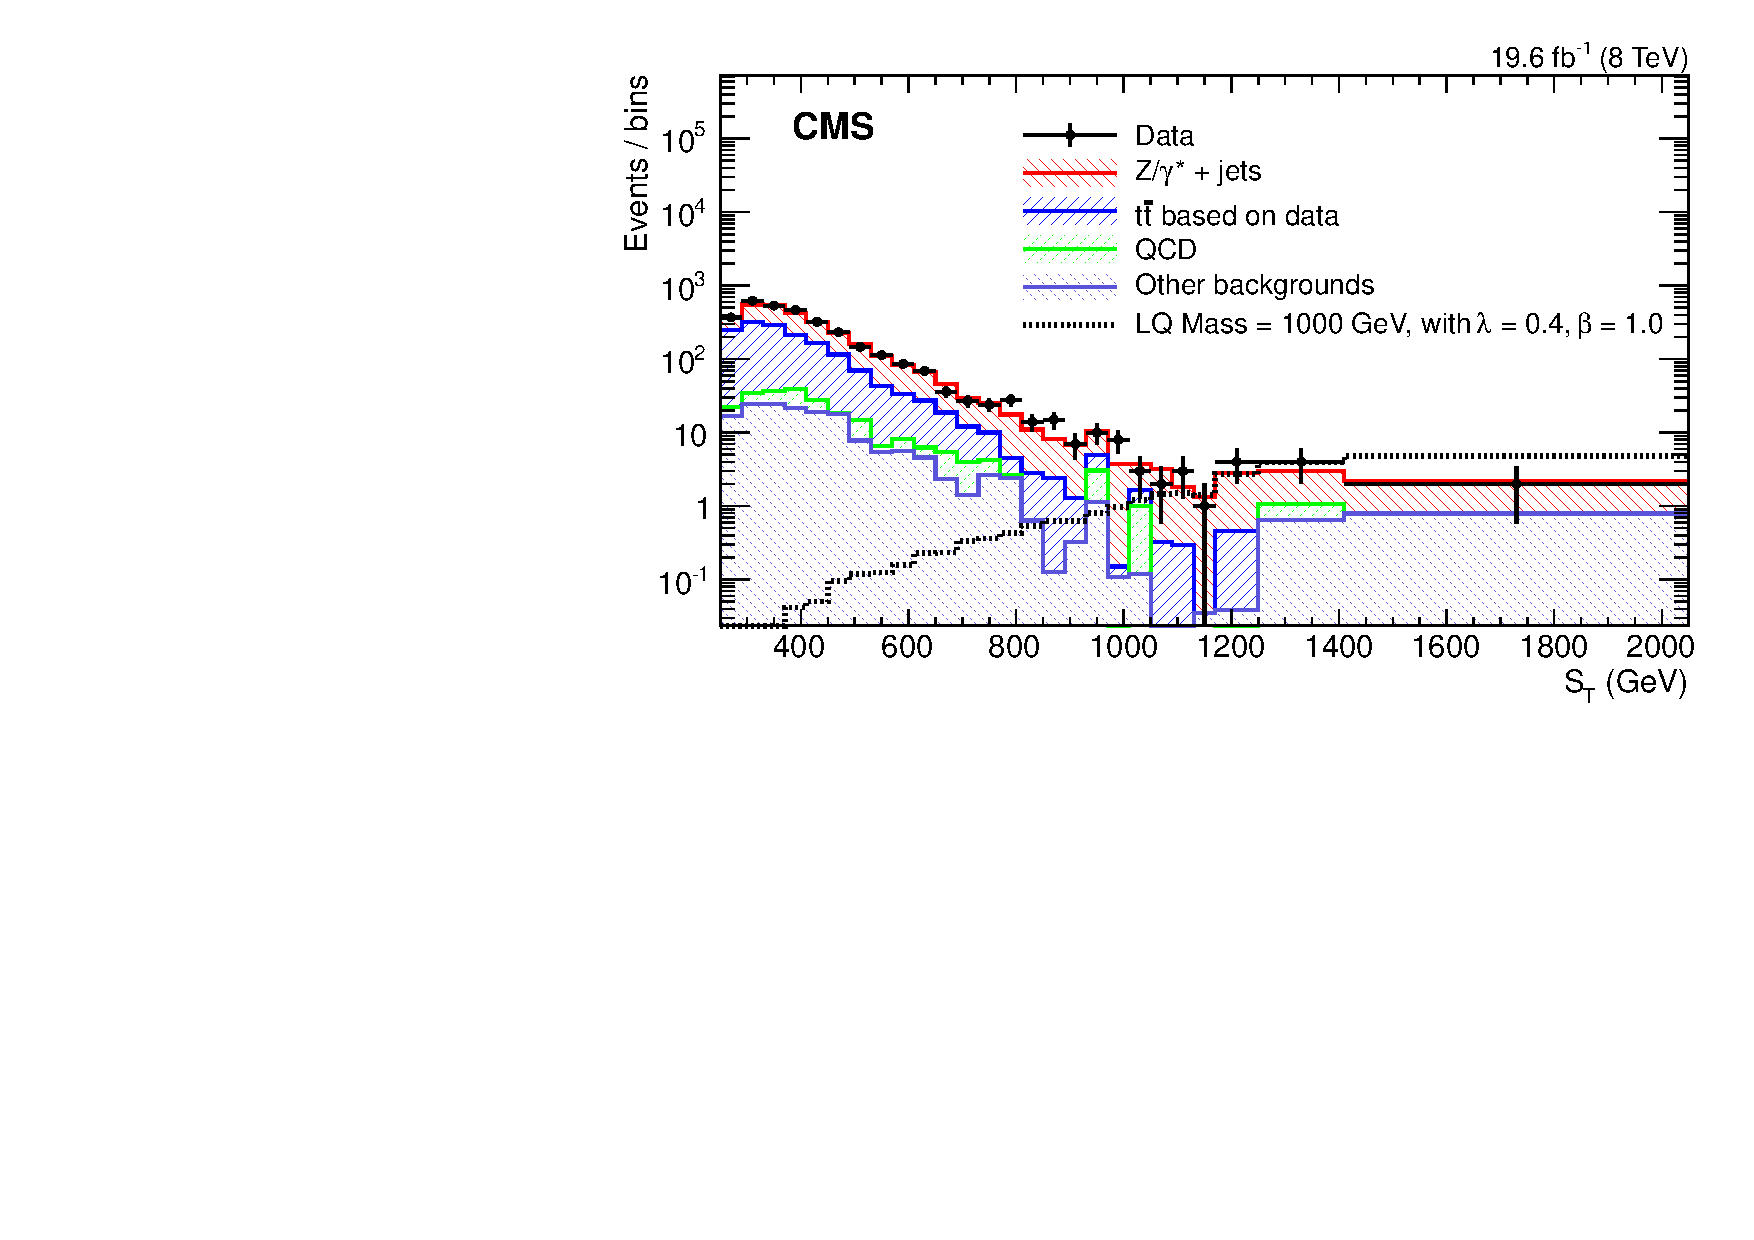
\includegraphics[width=.75\textwidth]{Figures/Figures_ee_ST_pf_ee_single_Preselection.pdf}}
       {\includegraphics[width=.75\textwidth]{Figures/Figures_ee_M_singleLQ_epfjet_Masshigh_Preselection.pdf}}
       \caption{Distributions of $M_{\Pe \Pe}$ (top), $\ST$ (middle), and $M_{\Pe j}$ (bottom) at preselection in the $\Pe \Pe j$ channel.  ``Other backgrounds'' include diboson, \PW $+$ jets, and single top quark contributions.  The points represent the data and the stacked histograms show the expected background contributions.  The open histogram shows the prediction for an LQ signal for $M_{\text{\text{LQ}}}$ = 1000\GeV and $\lambda=0.4$.  The horizontal error bars on the data points represent the bin width.  The last bin includes overflow. \label{figapp:elemisc}}
\end{figure}

\begin{figure}[!htb]
       \centering
       {\includegraphics[width=.75\textwidth]{Figures/Figures_mumu_M_muon1muon2_Preselection.pdf}}
       {\includegraphics[width=.75\textwidth]{Figures/Figures_mumu_ST_pf_mumu_single_Preselection.pdf}}
       {\includegraphics[width=.75\textwidth]{Figures/Figures_mumu_M_singleLQ_mupfjet_Masshigh_Preselection.pdf}}
       \caption{Distributions of $M_{\Pgm \Pgm}$ (top), $\ST$ (middle), and $M_{\Pgm j}$ (bottom) at preselection in the $\Pgm \Pgm j$ channel.  ``Other backgrounds'' include diboson, \PW $+$ jets, single top quark, and QCD multijet contributions.  The points represent the data and the stacked histograms show the expected background contributions.  The open histogram shows the prediction for an LQ signal for $M_{\text{\text{LQ}}}$ = 600\GeV and $\lambda=1.0$.  The horizontal error bars on the data points represent the bin width.  The last bin includes overflow. \label{figapp:muonmisc}}
\end{figure}

\begin{figure}[!htb]
       \centering
       {\includegraphics[width=.75\textwidth]{Figures/Figures_ee_ST_pf_ee_single_Fullselection.pdf}}
       {\includegraphics[width=.75\textwidth]{Figures/Figures_ee_M_singleLQ_epfjet_Masshigh_Fullselection.pdf}}
       \caption{Distributions of $\ST$ and $M_{\Pe j}$ at final selection, in the $\Pe \Pe j$ channel .  The points represent the data and the stacked histograms show the expected background contributions.  The open histogram shows the prediction for an LQ signal for $M_{\text{\text{LQ}}}=1000\GeV$ and $\lambda=0.4$.  The horizontal error bars on the data points represent the bin width.  The last bin includes overflow. \label{figapp:elefinalsel}}
\end{figure}

\begin{figure}[!htb]
       \centering
       {\includegraphics[width=.75\textwidth]{Figures/Figures_mumu_ST_pf_mumu_single_Fullselection.pdf}}
       {\includegraphics[width=.75\textwidth]{Figures/Figures_mumu_M_singleLQ_mupfjet_Masshigh_Fullselection.pdf}}
       \caption{Distributions of $\ST$ and $M_{\Pgm j}$ at final selection, in the $\Pgm \Pgm j$ channel.  The points represent the data and the stacked histograms show the expected background contributions.  The open histogram shows the prediction for an LQ signal for $M_{\text{\text{LQ}}}=600\GeV$ and $\lambda=1.0$.  The horizontal error bars on the data points represent the bin width.  The last bin includes overflow. \label{figapp:mufinalsel}}
\end{figure}

\section{Systematic uncertainties}
\label{systematics}

The sources of systematic uncertainties considered in this analysis are listed below.  To determine the uncertainties in signal and background, each kinematic quantity listed is varied individually according to its uncertainty and the final event yields are re-measured to determine the variation in the predicted number of background and signal events.

Jet energy scale and resolution uncertainties are estimated by assigning $\PT$- and $\eta$-dependent uncertainties in jet energy corrections as discussed in Ref.~\cite{CMS-PAPERS-JME-10-011}, and varying the jet $\PT$ according to the magnitude of that uncertainty.  The uncertainty in the jet energy resolution is assessed by modifying the $\PT$ difference between the particle level and reconstructed jets by an $\eta$-dependent value between 5\% and 30\% for most jets~\cite{CMS-PAPERS-JME-10-011}.  

Uncertainties in the charged-lepton momentum scale and resolution also introduce uncertainties in the final event acceptance.  An energy scale uncertainty of 0.6\% in the ECAL barrel and 1.5\% in the ECAL endcap is assigned to electrons~\cite{EleUncertainties}, and an uncertainty of 10\% in both the ECAL barrel and endcap is applied to the electron energy resolution~\cite{EleUncertainties}.  There is an uncertainty of 0.6\% per electron in reconstruction, identification, and isolation requirements.  For muons, a $\PT$-dependent scale uncertainty of  $5\% \, (\PT/1 \TeV)$ is applied, as well as a 1--4\% $\PT$-dependent resolution uncertainty~\cite{Chatrchyan:2012xi}.  In the case of momentum scale uncertainties the momentum is directly varied, and in the case of momentum resolution uncertainties the lepton momentum is subjected to a Gaussian random smearing within the uncertainty.  A 2\% per muon uncertainty in reconstruction, identification, and isolation requirements, as well as a 1\% muon HLT efficiency uncertainty, are assumed as well.

Other important sources of systematic uncertainty are related to the modeling of the backgrounds in the simulation.  The uncertainty in the $\cPZ/\gamma^{*}$ $+$ jets background shape  is determined by using simulated samples with renormalization and factorization scales and matrix-element parton-shower matching thresholds varied by a factor of two up and down.  The scale factors for the normalization of the $\cPZ/\gamma^{*}+$ jets background are assigned an uncertainty of 0.6\% in both channels and the normalization of the \ttbar background is assigned an uncertainty of 0.5\% in both channels, from the studies in Section~\ref{backgrounds}, with an additional uncertainty of 4\% applied to the $\ttbar$ background normalization in the $\Pgm \Pgm j$ channel to account for possible signal contamination from first generation LQs in the control sample (the contamination is extremely small in the other channel because of the suppressed second generation signal).  An uncertainty on $\cPZ/\gamma^{*}+$ jets background from the $\PT(\ell\ell)$ scale factors is assessed by taking the weighted average of the uncertainties from each $\PT(\ell\ell)$ bin.  The estimate of the QCD multijet background from data has an uncertainty of 15\%.

An uncertainty in the modeling of pileup in simulation is determined by varying the number of simulated pileup interactions up and down by 6\%~\cite{pileupuncert}, and an uncertainty of 2.6\% on the measured integrated luminosity is applied~\cite{CMS-PAS-LUM-13-001}.

Uncertainties in the signal acceptance, the background acceptance, and the cross sections, due to the PDF choice of 4--10\% for signal and 3--9\% for background are applied, following the PDF4LHC recommendations described in Refs.~\cite{PDF4LHC,Alekhin:2011sk}.

Finally, a statistical uncertainty associated with the size of the simulated sample is included for both background and signal. 

The systematic uncertainties are listed in Table~\ref{tab:systs}, together with their effects on signal and background yields, corresponding to the final selection values optimized for $M_{\text{LQ}} = 600$ \GeV.  The PDF uncertainty is larger in the $\Pgm \Pgm j$ channel because of the large uncertainty associated with the $\PQs$-quark PDF.

\begin{table}
\caption{Systematic uncertainties (in \%) and their effects on total signal (S) and background (B) in both channels for $M_{\text{LQ}} = 600$ \GeV final selection.}
\centering
\begin{tabular}{lcccc}
{Systematic} & \multicolumn{2}{c}{$\Pe \Pe j$} & \multicolumn{2}{c}{$\Pgm \Pgm j$}\\
{uncertainty} & {S(\%)} & {B(\%)} & {S(\%)} & {B(\%)}\\
\hline
{Jet energy scale} & {0.3} & {1.0} & {0.7} & {1.4}\\
{Jet energy resolution}  & {0.1} & {0.3}  & {0.3} & {0.4}\\
{Electron energy scale}  & {0.2} & {2.1} & {-} & {-}\\
{Electron energy resolution}  & {0.1} & {0.6} & {-} & {-}\\
{Muon energy scale}  & {-} & {-} & {2.4} & {3.7}\\
{Muon energy resolution}  & {-} & {-} & {0.2} & {1.1}\\
{Electron reco/ID/iso}  & {1.2} & {0.1} & {-} & {-}\\
{Muon reco/ID/iso}  & {-} & {-} & {2.0} & {0.1}\\
{Trigger}  & {-} & {-}  & {1.0} & {0.1}\\
{QCD normalization}  & {-} & {0.0} & {-} & {0.1}\\
{\ttbar normalization}  & {-} & {0.2}  & {-} & {1.1}\\
{$\cPZ/\gamma^* +{\rm jets}$ normalization}  & {-} & {0.3} & {-} & {0.3}\\
{$\cPZ/\gamma^* +{\rm jets}$ shape}  & {-} & {5.2} & {-} & {5.6}\\
{$\cPZ/\gamma^* +{\rm jets}$ $\PT(\ell\ell)$ scale factor}  & {-} & {2.6} & {-} & {3.0}\\
{PDF}  & {3.5} & {3.0}  & {3.0} & {2.8}\\
{Pileup}  & {2.5} & {0.6} & {2.8} & {1.9}\\
{Integrated luminosity} & {2.6} & {0.3} & {2.6} & {0.2}\\
{Statistical uncertainty} & {1.3} & {3.5} & {1.4} & {4.3}\\
\hline
{Total}  & {5.3} & {8.1}  & {6.05} & {8.1}\\
\end{tabular}
\label{tab:systs}
\end{table}

\section{Results}
\label{results}
The observed data are consistent with the no-signal hypothesis.  We set an upper limit on the leptoquark cross section by using the \CLS modified frequentist method~\cite{Read:2002hq,Junk:1999kv} with the final event yields.  A log-normal probability function is used to model the systematic uncertainties, whereas statistical uncertainties are described with gamma distributions with widths determined according to the number of events simulated or measured in data control regions.

To isolate the limits for resonant LQ production, we apply the resonant requirements at the generator level on both the lepton+jet mass, $M(\ell,j)> (0.67 \text{ or } 0.75 )\, M_{\text{LQ}}$ (for the first- or second- generation LQs, respectively), and on the dilepton mass, $M_{\ell \ell}> 110$\GeV.  These requirements make the limits extracted from data more conservative and are discussed in Section~\ref{selection}.  A resonant cross section $\sigma_{\text{res}}$ is computed with respect to those requirements.  Limits are then computed with the reduced sample of simulated signal events and compared to $\sigma_{\text{res}}$. 

The 95\% confidence level (\CL) upper limits on $\sigma_{\text{res}} \, \beta$ as a function of leptoquark mass are shown in Fig.~\ref{figapp:combinedlims} together with the resonant cross section predictions for the scalar leptoquark single production cross section.  The uncertainty band on the theoretical cross section prediction corresponds to uncertainties in the total cross section due to PDF variations with an additional $+70\%$ uncertainty, due to the k factor ~\cite{Hammett:2015sea}.  The observed limits are listed in Tables \ref{tab:optimizedcuts1p0} and \ref{tab:optimizedcutscmu} in the appendix.

\begin{figure}[!htbp]
       \centering
       {\includegraphics[width=.75\textwidth]{Figures/Figures_ee_FiducialLimits_UEExclusion_1p0.pdf}}
       {\includegraphics[width=.75\textwidth]{Figures/Figures_mumu_FiducialLimits_Mu_Exclusion.pdf}}
       \caption{Expected and observed upper limits at 95\%~\CL on first and second generation leptoquark single production resonant cross section as a function of the leptoquark mass.  First generation limits are shown on the top plot with a resonant region of $M_{\ell j} > 0.66 \, M_{\text{LQ}}$, $M_{\ell \ell}> 110$\GeV and second generation limits are shown on the bottom plot with a resonant region of $M_{\ell j} > 0.75 \, M_{\text{LQ}}$, $M_{\ell \ell}> 110$\GeV.  The uncertainty bands on the observed limit represent the 68\% and 95\% confidence intervals.  The uncertainty band on the theoretical cross section includes uncertainties due to PDF variation and the k factor.\label{figapp:combinedlims}}
\end{figure}

By comparing the observed upper limit with the theoretical production cross-section times branching fraction, we exclude single leptoquark production at 95\% ~\CL for LQ masses below the values given in Table~\ref{figapp:limitstable}.

\begin{table}[!htbp]
\caption{95\% ~\CL lower limits on scalar LQ masses ($\beta = 1.0$).}
\centering
\begin{tabular}{rc}
LQ generation, coupling & Excluded mass (\GeVns) \\
\hline
{First gen., $\lambda=0.4$} & {   860} \\
{First gen., $\lambda=0.6$} & {1175} \\
{First gen., $\lambda=0.8$} & {1355} \\
{First gen., $\lambda=1.0$} & {1755} \\
{Second gen., $\lambda=1.0$} & {     660} \\
\end{tabular}
\label{figapp:limitstable}
\end{table}

Limits on single production of the $S^{R}_{0}$ type LQ from the H1 collaboration exclude LQ production up to 500\GeV ($\lambda=1.0$) and up to 350\GeV ($\lambda=0.6$)~\cite{Collaboration:2011qaa}.

 


%% Chapter 1

\chapter{Theory} % Main chapter title

\label{theory} % For referencing the chapter elsewhere, use \ref{Chapter1} 

\lhead{Chapter 1. \emph{Chapter Title Here}} % This is for the header on each page - perhaps a shortened title

%----------------------------------------------------------------------------------------

\section{The Standard Model}
 
%\input{Chapters/Chapter6} 
%\input{Chapters/Chapter7} 

%----------------------------------------------------------------------------------------
%	THESIS CONTENT - APPENDICES
%----------------------------------------------------------------------------------------

\addtocontents{toc}{\vspace{2em}} % Add a gap in the Contents, for aesthetics

\appendix % Cue to tell LaTeX that the following 'chapters' are Appendices

% Include the appendices of the thesis as separate files from the Appendices folder
% Uncomment the lines as you write the Appendices

% Appendix A

\chapter{Appendix Title Here} % Main appendix title

\label{AppendixA} % For referencing this appendix elsewhere, use \ref{AppendixA}

\lhead{Appendix A. \emph{Appendix Title Here}} % This is for the header on each page - perhaps a shortened title

Write your Appendix content here.
%\input{Appendices/AppendixB}
%\input{Appendices/AppendixC}

\addtocontents{toc}{\vspace{2em}} % Add a gap in the Contents, for aesthetics

\backmatter

%----------------------------------------------------------------------------------------
%	BIBLIOGRAPHY
%----------------------------------------------------------------------------------------

\label{Bibliography}

\lhead{\emph{Bibliography}} % Change the page header to say "Bibliography"

\bibliographystyle{unsrtnat} % Use the "unsrtnat" BibTeX style for formatting the Bibliography
%\bibliographystyle{plainnat} % Use the "unsrtnat" BibTeX style for formatting the Bibliography

\bibliography{Bibliography} % The references (bibliography) information are stored in the file named "Bibliography.bib"

\end{document}  
